\chapter[Evaluation of Cloud Cuts on Auger Event Data]{\centering Evaluation of Cloud Cuts on Auger Event Data \\}\label{Ch:CloudCuts}

This is an initial look into the effectiveness of the cloud cuts on reconstructed Fluorescence Detector events from 2004 to 2018. The set was restricted to Golden Hybrid events which are detected events that have both an FD and SD reconstruction available. The cloud cut described here are part of a series of quality cuts used to produce datasets for the ICRC 2019 conference. These series of quality cuts are used produce standardised datasets across the collaboration. I investigated the effects of removing the cloud cut from this series of quality cuts and quantify the effects of removal through the Elongation Rate and the Xmax distributions. Within this chapter I show the series of quality cuts used for this analysis.

%The cloud cut is just one of a series of quality cuts that are used to create sets of event that are ready for further analysis. The list  I investigated the effects of removing the cloud cut from this list of quality cuts and quantify the effects of removal through the Elongation Rate and the Xmax distributions. This list includes cuts to remove events within known bad data taking periods, cuts on aerosol levels, event quality etc. 

This investigation was done to quantify the effects that the cloud cuts had on the data set. A question had been raised about whether the quality cuts on fitted values, constraining the  $\chi^2$ and requiring events without large gaps were doing the same job as the cloud cuts. There is a lot of uncertainty about whether a detected cloud had impacted each event due to the time spacing of atmospheric measurements. The timing can sometimes vary between 5 and 15 minutes when measurements are available or larger if  atmospheric data is missing. Another reason to see if the other quality cuts are doing a similar job as the cloud cut is to help when cloud measurements are unavailable. There are multiple different cloud detection sources but none are prefect. It would be great to have alternative that can cover the rare times when we do not have atmospheric cloud measurements.

It is important to know where clouds are located in relation to EAS events due to the different effects that clouds can have on the detected light profile by the FDs. If a cloud partially obscures the FD view of the event it can cause a gap in the profile or a cloud may be in the path of the development of the EAS event. In the first case a gap will cause the reconstruction of the energy of the event to be underestimated. In the second case a cloud within the path of development can amplify the amount of Cherenkov light scattered towards the FD which can in turn cause an overestimate of the reconstructed energy.

Cloud information has large uncertainty about quantities like cloud height, distance from telescopes and timing. The main uncertainty is due to time gaps between data taken of the atmosphere. Examples of this are that cloud camera scans are performed every 5 minutes. Since this a snapshot, a cloud could move quite a far distance within this time spacing and introduce a large uncertainty.

\section{Equipment used to monitor clouds above the array} \label{sec:MonitoringEquipment}



\begin{figure}[!t]
\begin{subfigure}[b]{0.3\textwidth}
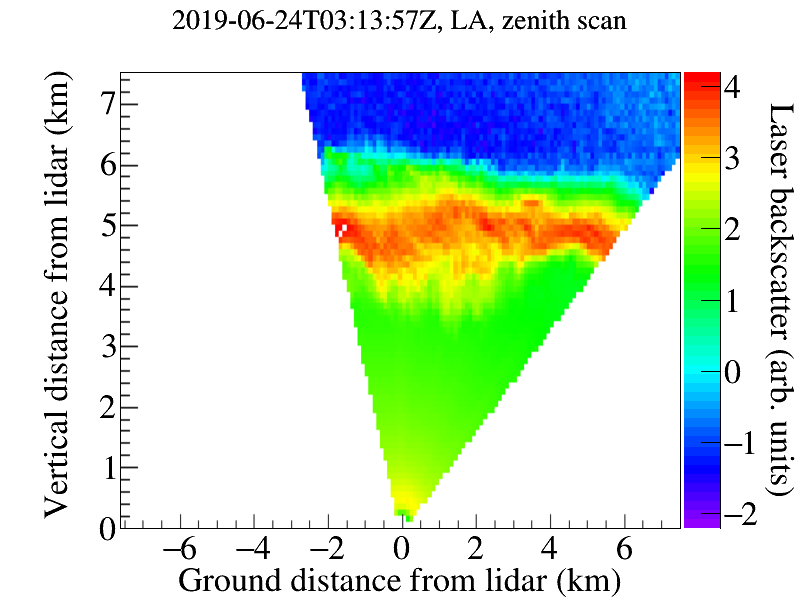
\includegraphics[width=\textwidth]{chapters/graphs/CloudFlags/lidar_scan.png}
\caption{} \label{subfig:liadr_scan}
\end{subfigure}
\begin{subfigure}[b]{0.3\textwidth}
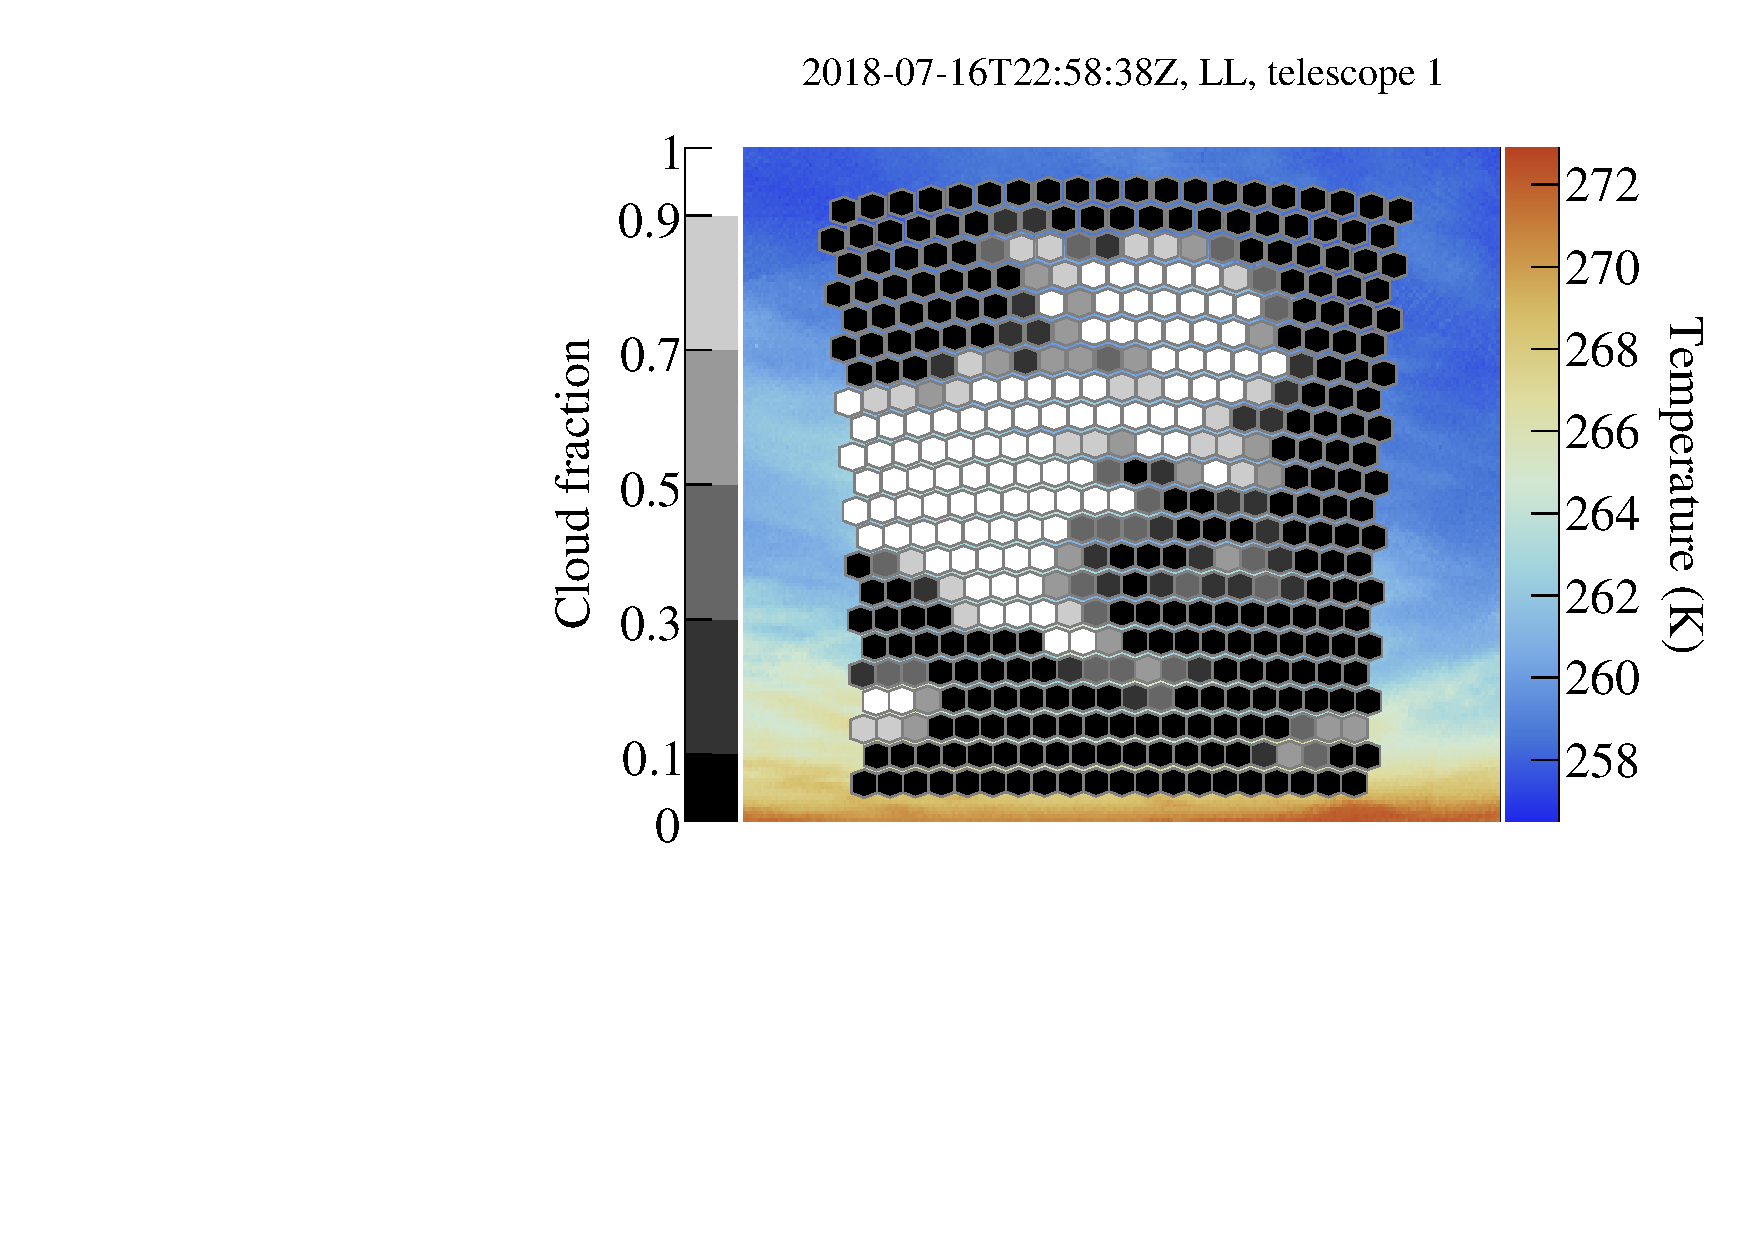
\includegraphics[width=\textwidth]{chapters/graphs/CloudFlags/ir_cloudfraction_pixels.pdf}
\caption{} \label{subfig:IR_cloudcam}
\end{subfigure}
\begin{subfigure}[b]{0.3\textwidth}
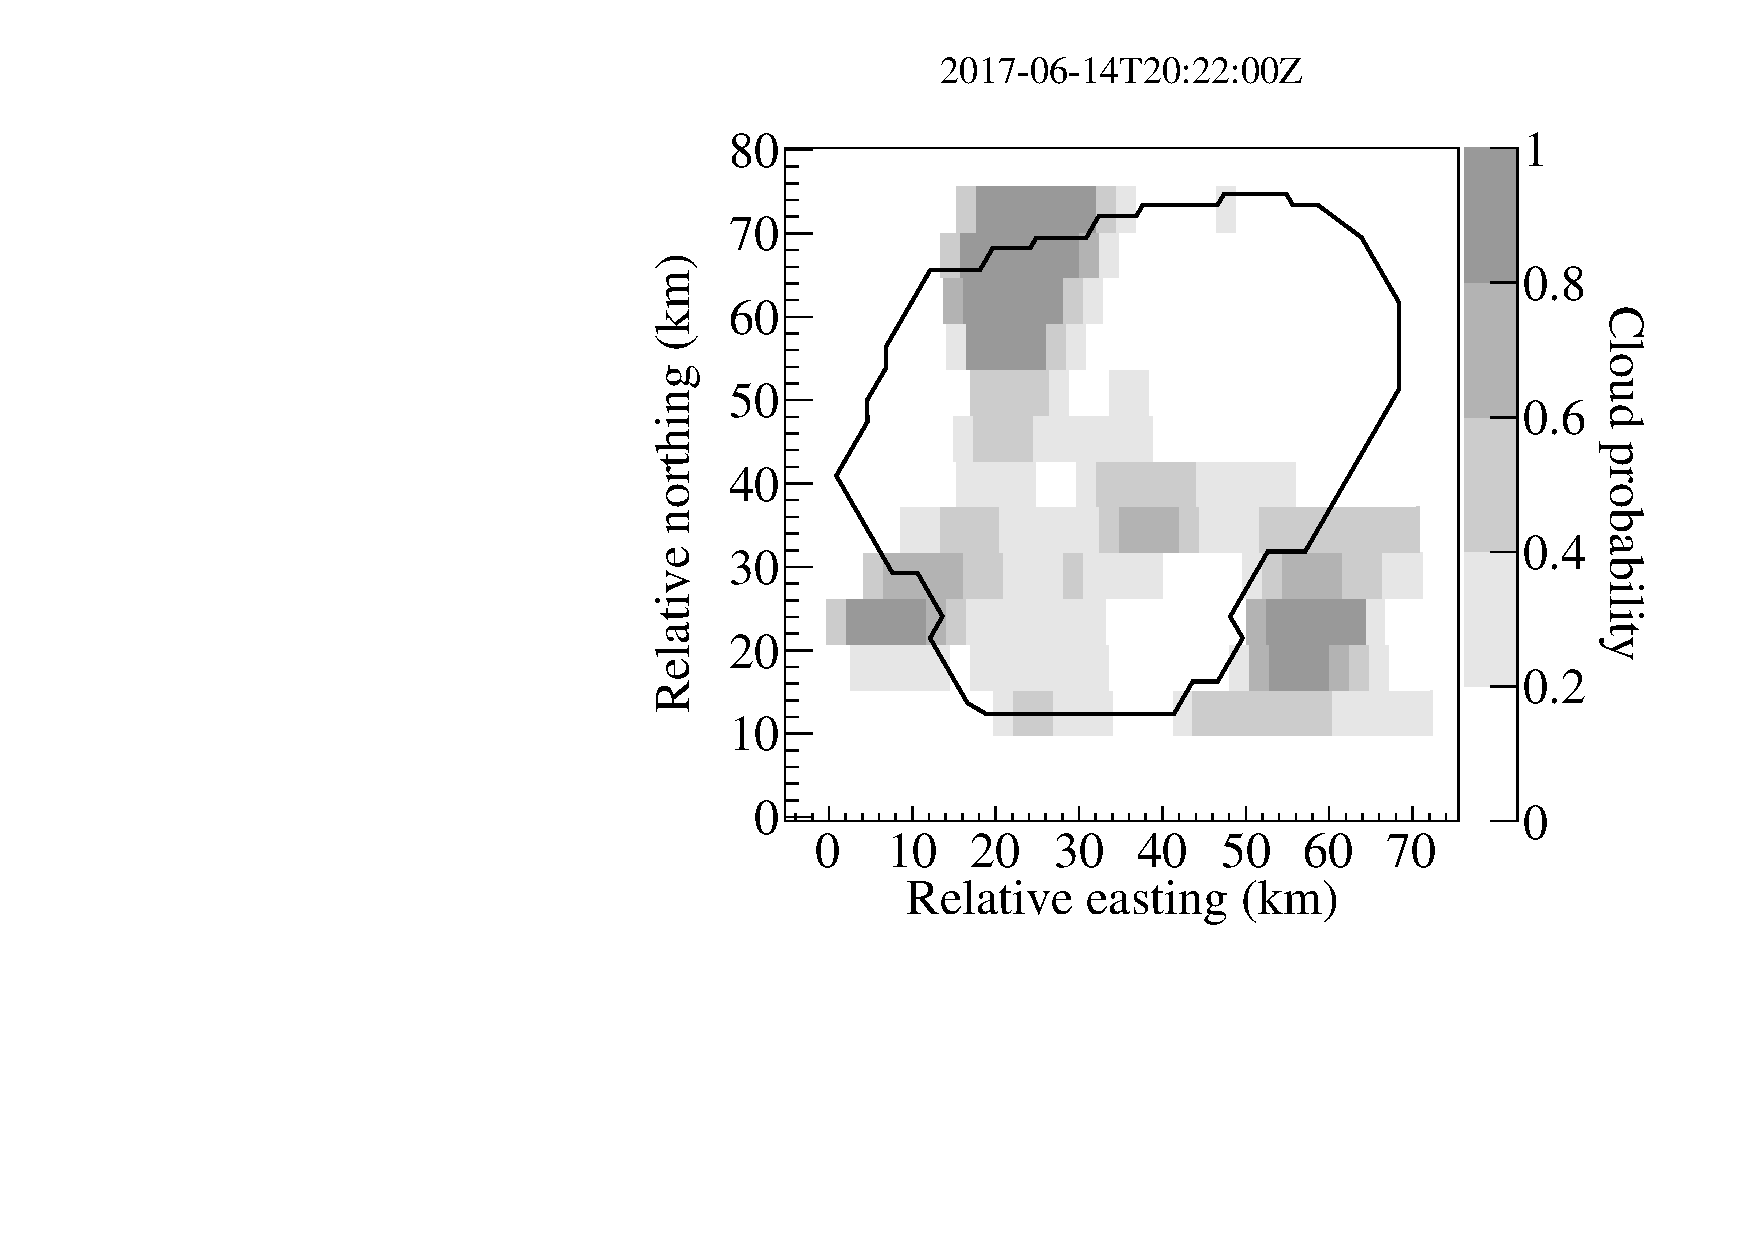
\includegraphics[width=\textwidth]{chapters/graphs/CloudFlags/ir_cloudprobability_map.pdf}
\caption{} \label{subfig:GOES}
\end{subfigure}
\caption{Examples of real data from (a) FD lidar scan, (b) cloud camera mask mapped to each pixel of a single FD telescope and (c) GOES cloud probability map covering the entire array.  Images provide by permission by V. Harvey.}
\end{figure}

There are multiple instruments used to monitor the cloud coverage across the array. These are a combination of collaboration run instruments specifically set-up to monitor atmospheric conditions within the array and externally run instruments that monitor broader atmospheric conditions that happen to include the array. The combination of instruments used to monitor clouds are the lidar system and infra-red cameras at each FD site, the Geostationary Operational Environmental Satellite (GOES) system, and the Central Laser Facility (CLF) and the eXtreme Laser Facility.

 
\subsection{Lidar System, Central Laser Facility and eXtreme Laser Facility}

There are three sets of lidar systems that are used to monitor the atmospheric conditions above the array. These sets are the monostatic elastic backscatter lidar deployed behind each of the FD telescope sites, the Central Laser Facility (CLF) and the eXtreme Laser Facility (XLF).

The monostatic elastic backscatter lidar is programmed to scan the sky above the FD field of view every 15 minutes. it works on the principle of measuring the time delay and magnitude of the returned signal to determine the distance and density of scattering centres. Both a minimum cloud base height (CBH) and percentage of overhead cloud coverage can be calculated. The overall CBH is an hourly average of all the 15 minute scans from all the FD sites. An example of a returned signal map is shown in Figure \ref{subfig:liadr_scan}. This example shows an overhead scan which indicates a localised cloud base height (CBH) of 4 km. The CBH and percentage of overhead cloud coverage is used when considering whether an event can be used in different analyses within Auger.


The CLF and the XLF's main purpose is to measure the atmospheric aerosol content but can be used to detect clouds either directly above the lasers or between the path of the laser and an FD site. A CBH can be determined for clouds detected directly above the laser or a lower limit can be determine if a cloud is detected between the laser and an FD site. The average CBH for an hour period is determined by the lowest CBH for any laser to FD pair measured within the hour.


\subsection{Infra-Red Cameras}

The main monitoring cloud system used is the infra-red cameras located on the roof of each of the FD sites. The cameras record light between 8 $\mu$m and 14 $\mu$m which measures clouds as warmer then the sky. The cloud cameras take images of the FoV of the FD eyes every 5 minutes while a full sky scan is performed every 15 minutes. The images within the FoV of the FD eyes are analysed to calculate a cloud fraction between 0\% and 100\% for each of the FD pixels. An example of the cloud mask being mapped to individual FD pixels is shown in Figure \ref{subfig:IR_cloudcam}. The pixels observing $\sim$ 5\textdegree \ elevation and below are not assigned a cloud fraction as observing clouds this close to the ground is difficult. The difficulty arises due to the fact that in IR the atmosphere becomes optically thick close to the horizon and the large present of water vapour close to the ground. When an event is reconstructed, the cloud fraction of each FD pixel that observed the EAS event is queried.

\subsection{Geostationary Operational Environmental Satellite (GOES) system}

The Geostationary Operational Environmental Satellite system (GOES) is operated by the United States National Oceanic and Atmospheric Administration. Auger uses the raw data that is publicly available and has created an algorithm to convert the aerial measurements across four IR bands to produce a cloud probability map every 30 minutes. An example of a GOES cloud probability map is shown in Figure \ref{subfig:GOES}. Each block represents a satellite pixel that covers an 2.4 km by 5.5 km area on the ground.

\section{Cloud Cuts employed on Auger data}

\begin{figure}[!t]
\centering
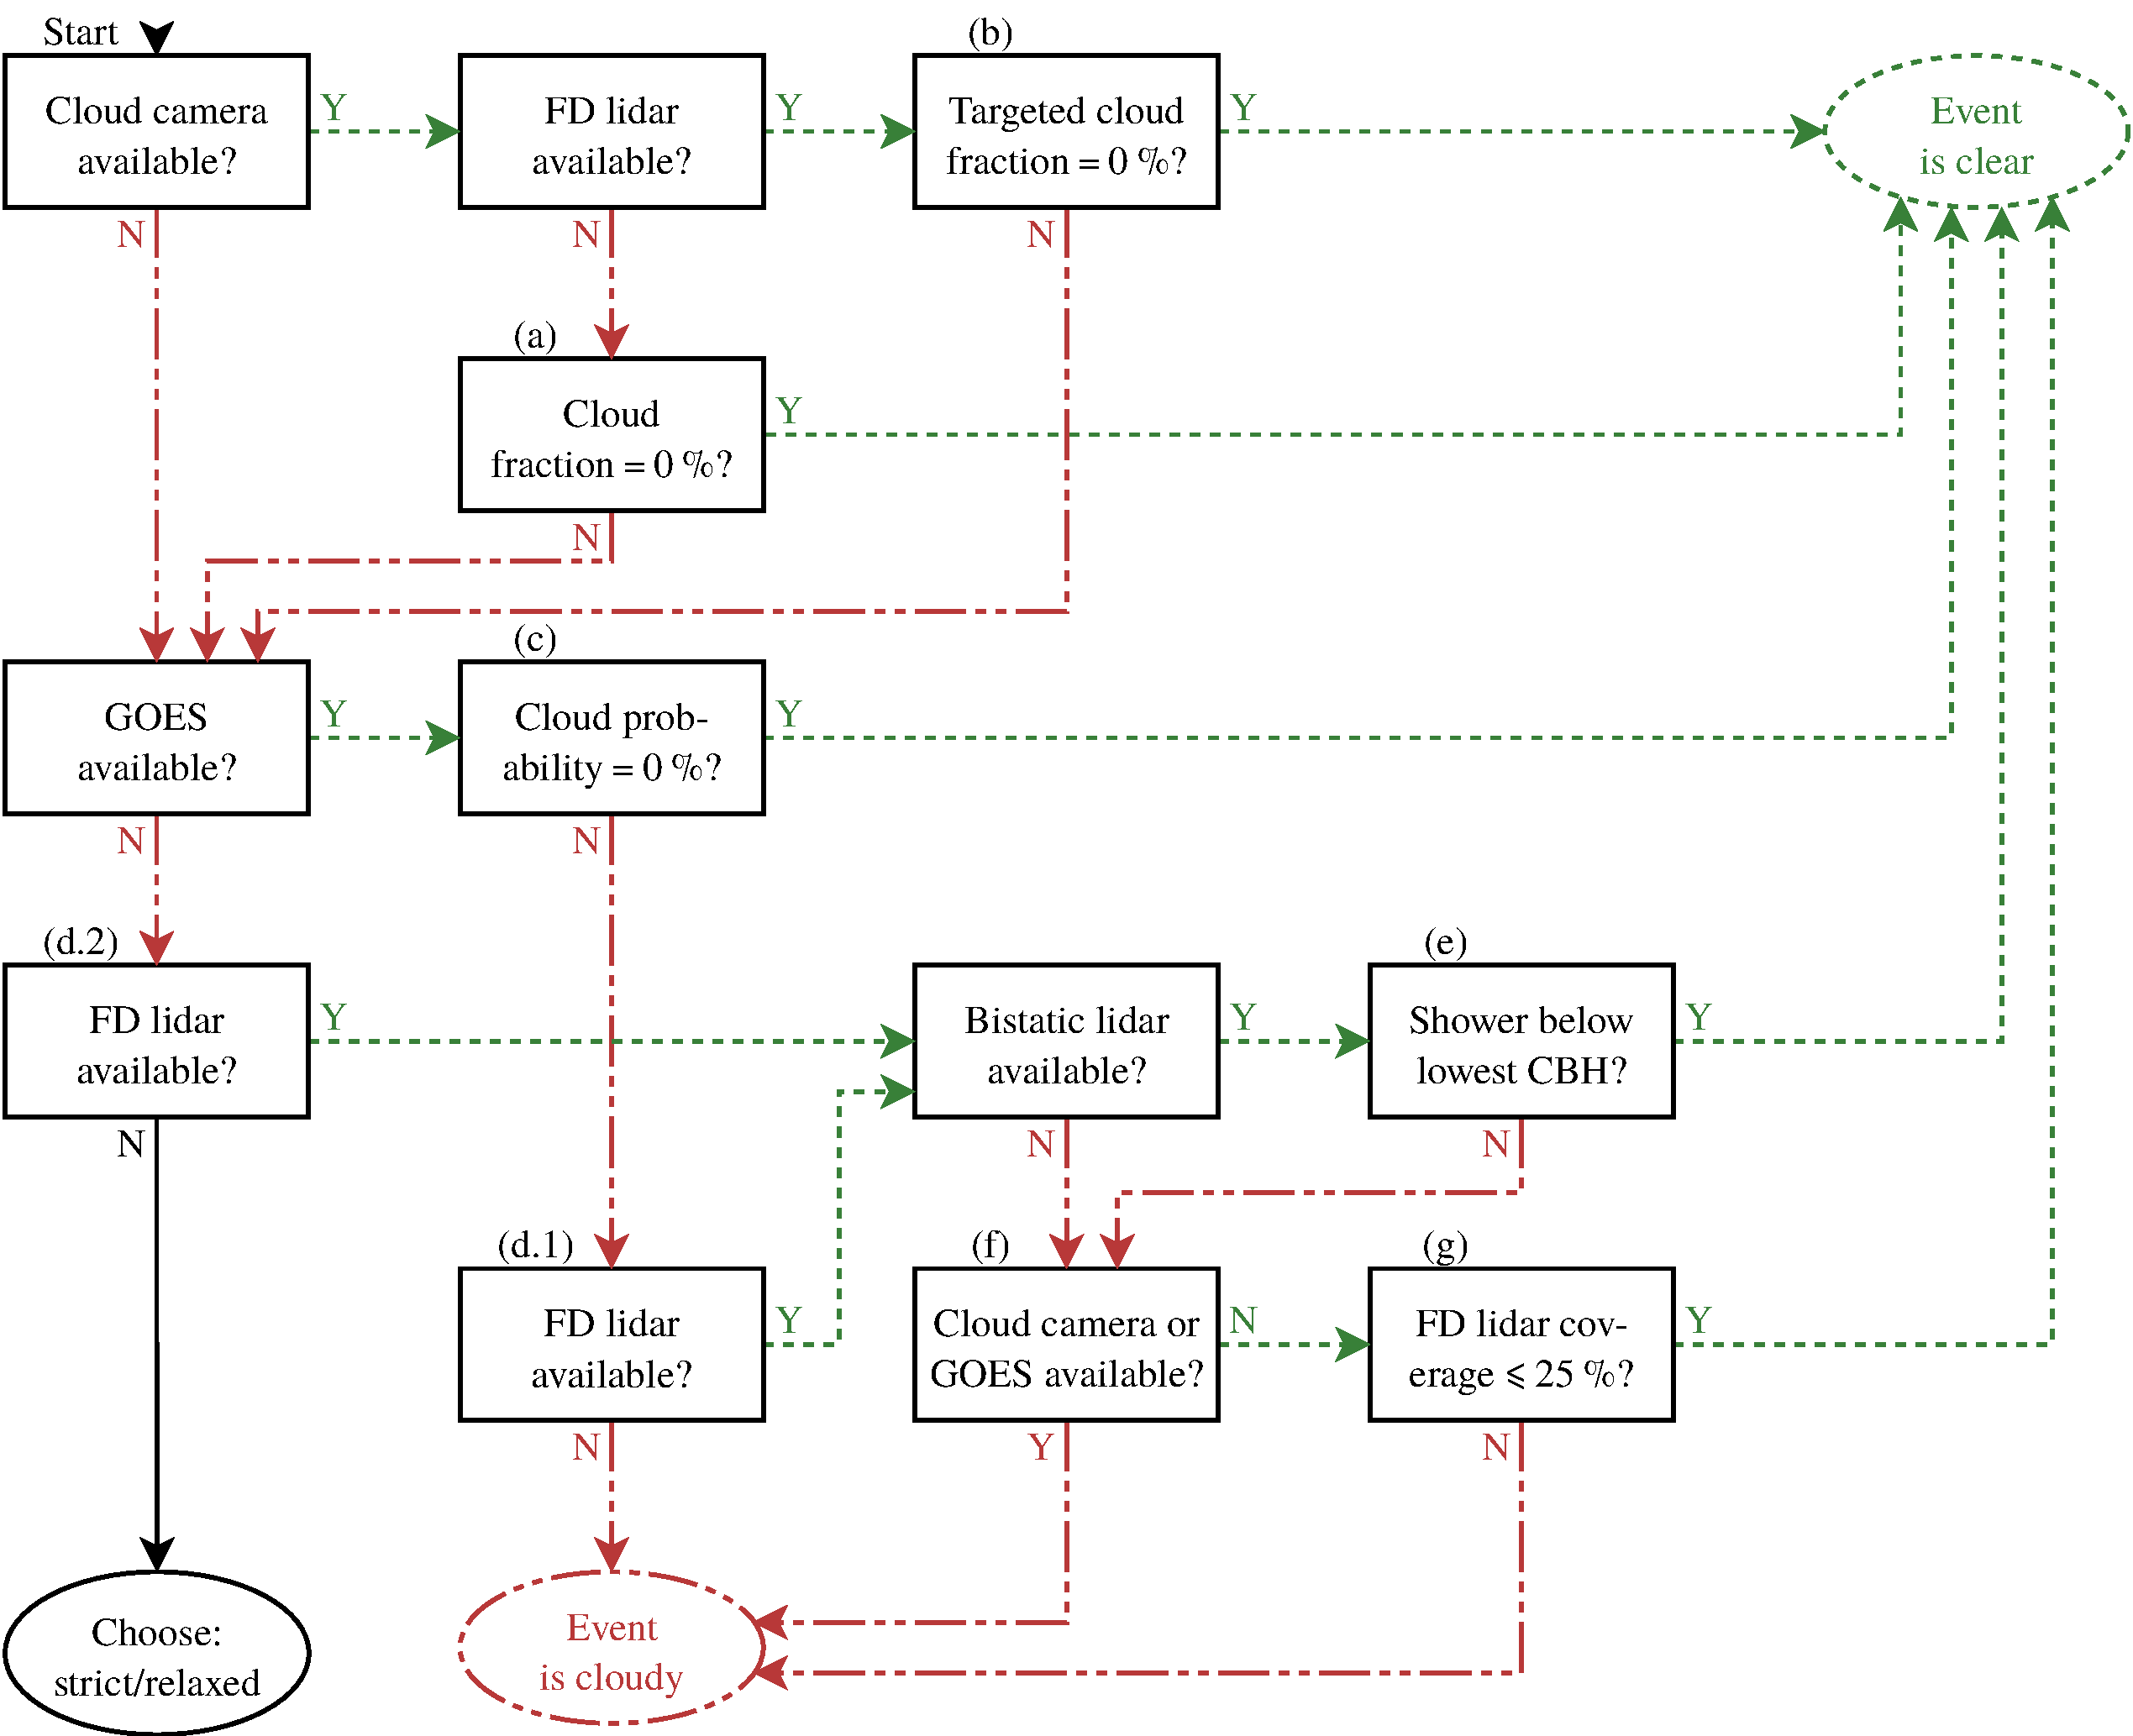
\includegraphics[width=0.7\textwidth]{chapters/graphs/CloudFlags/cloud_cuts.pdf}
\caption{Diagram of how the cloud cuts are applied to the data set when called with the Auger event selection program. Image provide by permission from V. Harvey} \label{fig:Cloud_Cut_Logic}
\end{figure}

Atmospheric measurements from the instruments described in Section \ref{sec:MonitoringEquipment} are processed and cloud probabilities are calculated. This data is then used within the Cloud cut to flag whether an event should be accepted or rejected. Within the Cloud cuts are checks to accommodate the multiple cloud data sources, both individually and in combination with each other. Figure \ref{fig:Cloud_Cut_Logic} shows the logic currently employed within the Cloud cut. The first check starts at (a) as go through to (f).  If an event passes a cut no further checks are performed.

\begin{itemize}
\item[(a)] If IR Cloud Mask is available for the pixels involved, an event will pass if there is 0\% cloud fraction. The cloud fraction is not calculated for pixel below 5.5\textdegree \ elevation. 
\item[(b)] Similar to step (a) but combines the nearest available FD lidar to determine the CBH to help whether the cloud is in front or behind the shower. The cloud mask fraction for pixels can be ignored if the CBH shows that the observed shower is below the cloud. Each pixel cloud fraction is recalculated and the event will pass if the total cloud fraction along the shower path is 0\%.
\item[(c)] If GOES data is available, this data is used to calculate the cloud probability between the FD site and the observed shower axis. If the cloud probability along the shower path is 0\% then the event will pass.
\item[(d)] No further steps are attempted if no FD lidar is available.
\begin{itemize}
\item[(d.1)] If all the above information is available and the event does not pass any of the cuts the event is flagged as being cloud effected.
\item[(d.2)] If none of the above information is available then the event cannot be flagged as either unaffected by could or not. The event is retained or discarded whether a "strict" or "relaxed" flag is set in the cloud cut settings. The relaxed setting is generally used but this is dependent on the analysis performed.
\end{itemize}
\item[(e)] If FD lidar and bistatic lidar data is available and no cloud camera or GOES information is available. The FD lidar and bistatics lidar can be used to determine the CBH. If the shower is below the lowest value of measured CBH the event will pass.
\item[(f)] If the event fails the condition in (e) or no data from the bistatic laser is available the event is checked to see if it has been flagged as cloudy by either the cloud camera or GOES data. If neither the cloud camera or GOES data is available then one last check is performed.
\item[(g)] The FD lidar data is used to determine the cloud coverage above the FD FoV. If the cloud coverage is less than 25\% the event is flagged as clear.
\end{itemize}



\section{Cloud Flags Investigation Method}

%Take reconstructed Golden Hybrid events from 2004 to 2018 
%
%Extract camera flag data.
%
%Two set of camera flags - positive ones that say that an event has pass one of the conditions saying that these is no cloud. the negative flags say that the event has failed to pass any of the test looking for clouds. If the flag is zero then there is no cloud information available.
%
%Four different flags - IR Cloud camera, LIDAR, GOES satellite data and something else.
%
%Look at the histograms of Xmax distributions for data passing cloud cuts, data failing cloud cuts and combined.

\begin{table}
\centering
\begin{tabular}{|c c|}
\hline 
\multicolumn{2}{|c|}{\textbf{==== reject laser events ====}} \\ \hline
!isCLF & \\
!isXLF & \\
\hline
\multicolumn{2}{|c|}{\textbf{==== keep either CO/HEAT or HECO ====}} \\ \hline
keepHECOorCoihuecoHEAT & 18.1 { nMinusOne: 21  -10.5 10.5 } \\
eyeCut & 1111 \\
\hline
\multicolumn{2}{|c|}{\textbf{==== hardware status ====}} \\ \hline
badFDPeriodRejection & \\
minMeanPixelRMSMergedEyes & {  params: 17 6 110000 nMinusOne: 100  0 100 } \\
minMeanPixelRMSSimpleEyes & {  params: 17 11111 nMinusOne: 100  0 100 } \\
!badPixels  &               1 \\
good10MHzCorrection & \\
\hline
\multicolumn{2}{|c|}{\textbf{==== atmosphere ====}} \\ \hline
hasMieDatabase & \\
maxVAOD & 0.1 \\
cloudCutXmaxPRD14  & { params: 1 nMinusOne: 21  -10.5 10.5 } \\
\hline
\multicolumn{2}{|c|}{\textbf{==== full hybrid geometry ====}} \\ \hline
hybridTankTrigger &       2 \\
maxCoreTankDist & 1500 \\
maxZenithFD       &        90 \\
minLgEnergyFD    &        1e-20 \\
skipSaturated & \\
minPBrass         &        0.9 \\
maxPBrassProtonIronDiff &  0.05 \\
minLgEnergyFD     &       17.8 \\
\hline
\multicolumn{2}{|c|}{\textbf{==== FOV cuts ====}} \\ \hline
FidFOVICRC13 & 40 20 \\
\hline
\multicolumn{2}{|c|}{\textbf{==== quality cuts ====}} \\ \hline
xMaxObsInExpectedFOV & { params: 40 20 } \\
maxDepthHole    &     20. \\
profileChi2Sigma  &  {  params:  3 -1.1 nMinusOne: 400  -20 20 } \\
depthTrackLength   &  200 \\ \hline
\end{tabular}
\caption{Relaxed cloud cut version of PRD14 cut} \label{tab:Quality_Cuts}
\end{table}


The method used to investigate the effects of the cloud cuts on the Auger data was applied to the Golden Hybrid data set with events from 2004 to 2018. First the events where reconstructed through the Auger OffLine program and then the reconstructed events where passed through a selectEvents program. This selectEvents program utilises a series of parameters to apply quality cuts to the reconstructed events. The list of cuts used are shown in Tab \ref{tab:Quality_Cuts}. The cuts used on the data set for the ICRC2019 list of cuts is taken from within the collaboration OffLine application. Once a standard set of events was produced, another set was produced where all of the cuts were applied except for the Cloud Cuts. 

After these two data sets where produced, I then took the code that would assign the cloud flag to an event and then used it within my own analysis code. The code was then used to apply a flag number to indicate which of the cloud cuts the event would pass or fail. I assigned a positive value between 1 and 5 to say that the event was cloud free. The number indicates which monitoring instrument said that there was no clouds between the event and the triggered Fluorescence Telescope (FD). A zero meant that there was no data from any monitoring instrument. A negative number was used to denote that the cloud data from the monitoring instrument indicated that the threshold was triggered to say that the event should be rejected. 

From there I looked into the Elongation Rate (Xmax vs log$_{10}$(Energy)) which is of concern for any study involving mass composition. I will show the distributions of events in log$_{10}$(Energy) and Xmax. The Xmax plots are split up into different energy bins to see the distributions. I was particularly interested in quantifying the tails of these distributions as they would be of most concern to the mass composition studies. Any mass composition analysis needs to have confidence in the calculation of the mean and standard deviation which is used to indicate the average composition of events within a particular energy bin. Removing or adding a quality cut is done with a lot of considerations in mind. Outside of mass composition, there will be other studies that are not as concerned with tails of the Xmax distributions.

I also show examples of individual events that would and would not pass the cloud cuts. This is to give a visual indication of what events that would pass look like and compare this to events that would fail the cloud cut. I have also shown some events that have weird properties which I will explain further within the results and discussion section.


\section{Results - Effect on Mean Xmax and Spread in Xmax}

%- Cloud Cut Flags distribution
%
%- Xmax distributions within energy bins
%
%- Elongation rate  
%
%- Is distance to Xmax or distance to shower axis needed?

\subsection{Cloud Flags Distribution}

Figure \ref{fig:cloudFlag_dist} shows the distribution of reconstruction shower events that would pass all quality cuts what Cloud Cut Flag has been assigned to them. Greater than zero means that the event has passed one of the cases to say that the event has a high probability it has not been effected by clouds. Less than zero means that the event has had a cloud detected close enough in space or time with a high probability to have had an effect. Minus one denotes events that have failed the cloud camera and/or the lidar condition, minus two denotes events that have failed the GOES data condition and minus three are events that have failed combinations of CLF/XLF, GOES data, Cloud camera and lidar conditions. Zero means that there is no definite measurement that the event has or has not been effected by clouds. Events with the zero flag are kept or discarded whether the relaxed or strict settings are used. In this case the relaxed setting was used so the events with flag equal to zero were marked as considered to not having any cloud.

\subsection{Elongation Rate}


\begin{figure}[!hp]
\centering
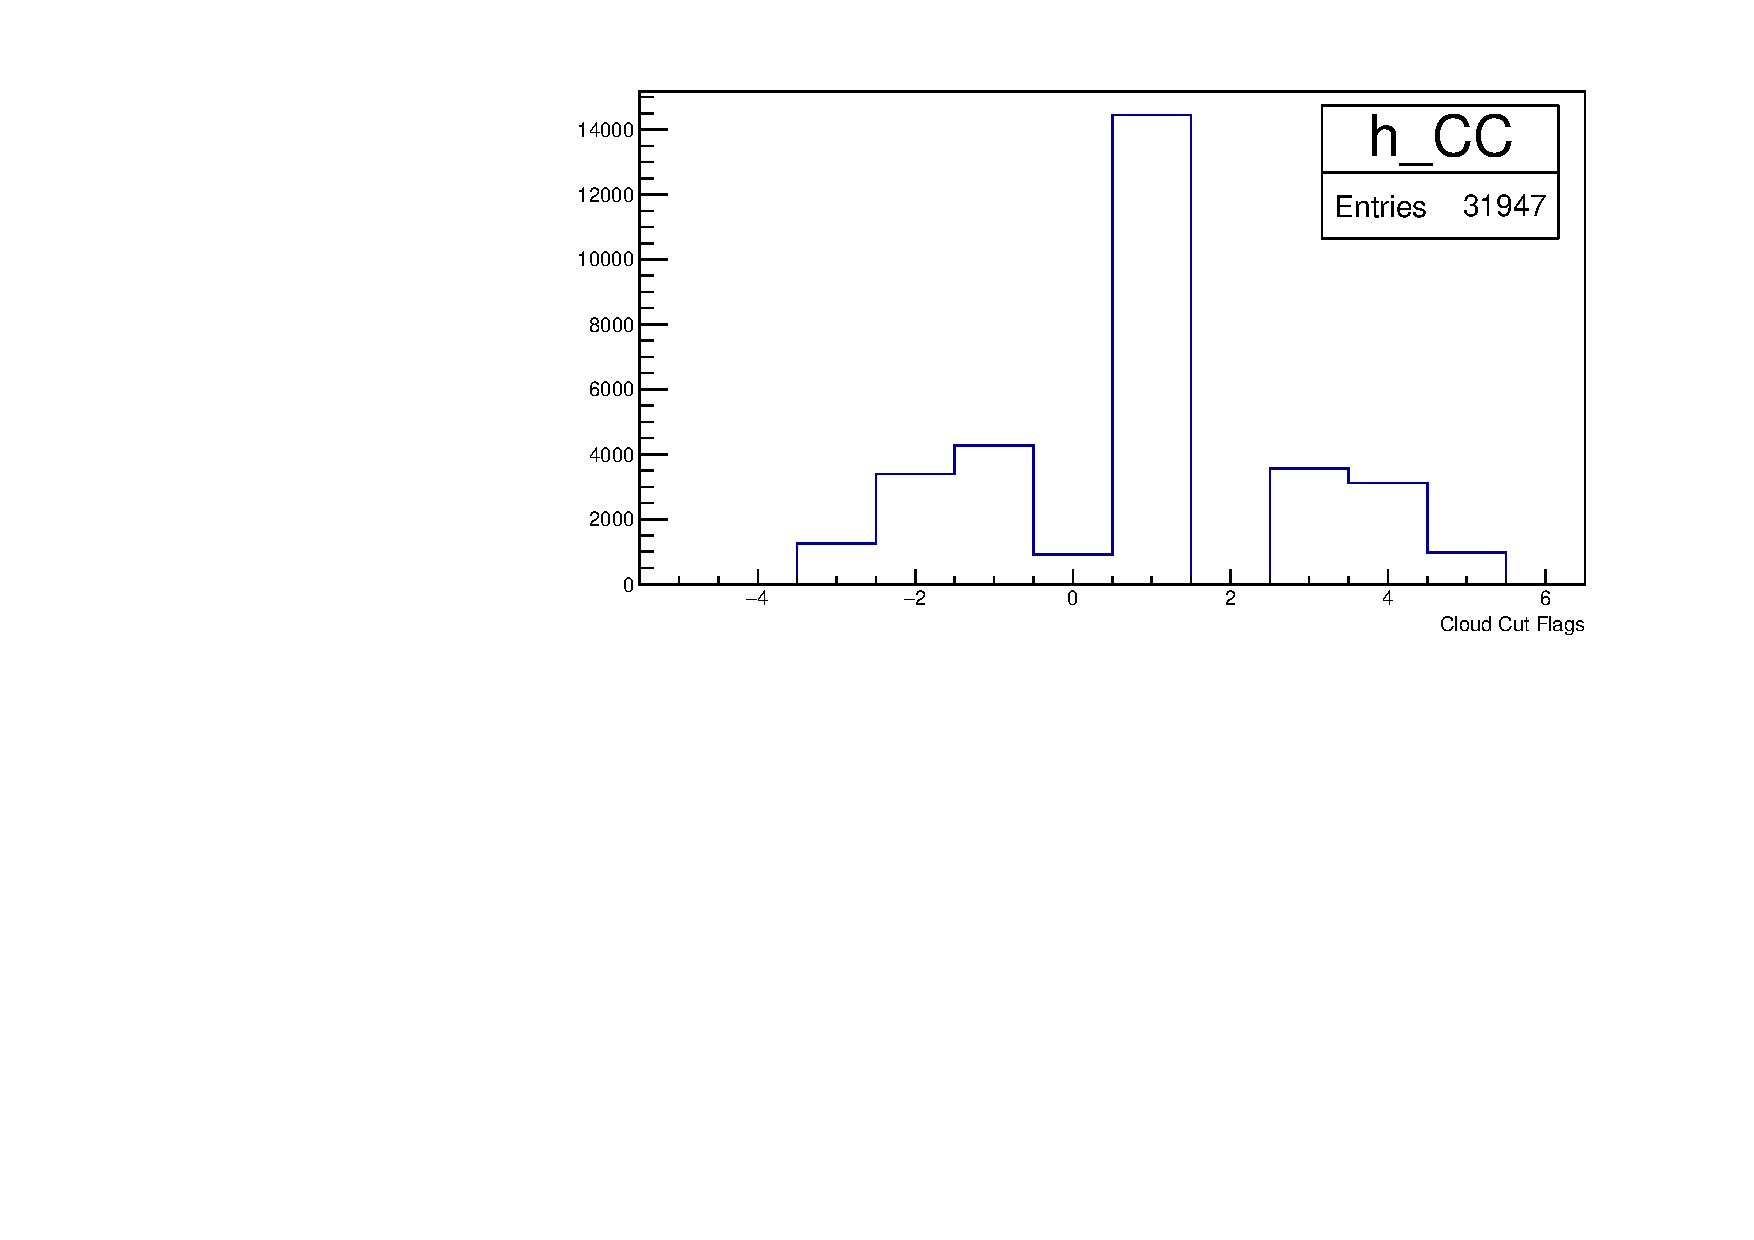
\includegraphics[width=\textwidth]{chapters/graphs/CloudFlags/hist_cloudFlags.pdf}
\caption{Distribution of cloud flags. Positive flag values are for events that would pass one of the cloud cuts. Negative flag values are for events that would fail one of the cloud cuts. A flag value of zero is for events that have no cloud data.}\label{fig:cloudFlag_dist}
\end{figure}

\begin{figure}[!hp]
\centering
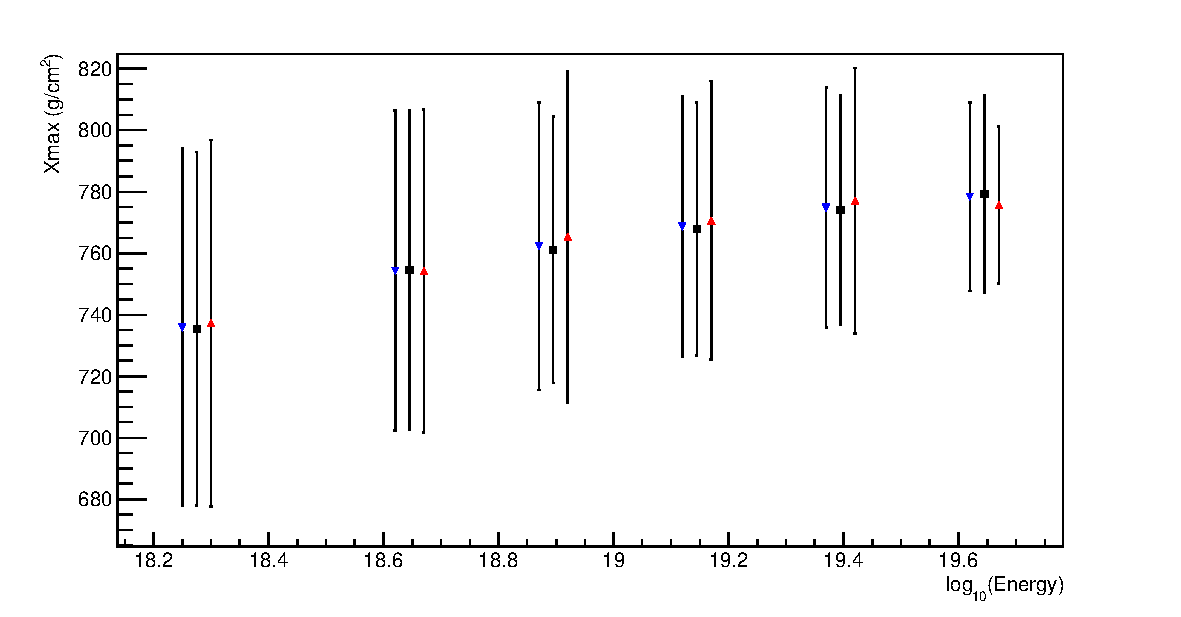
\includegraphics[width=\textwidth]{chapters/graphs/CloudFlags/ElongationRate.pdf}
\caption{Elongation Rate with Cloud cuts applied (blue downward triangle), without any cloud cuts (black square) and only events that would fail the cloud cuts (red upward triangle). The uncertainity bars denote the standard deviation of each distribution.} \label{fig:ElongRate_hist}
\end{figure}

Figure \ref{fig:ElongRate_hist} shows how the elongation rate as a function of energy. This figure shows the mean and standard deviation of Xmax within each energy bin. The standard deviation is shown as it is of importance to mass composition studies. There is no significance difference between the elongation  rates of the different data sets with Cloud Cuts applied (blue downwards triangles), without any Cloud Cuts (black squares) and only events that would fail the cloud cuts (red upward triangles).

% Energy Distribution

\subsection{Spectrum of events by Energy}

Comparison distributions of the energy spectrum observed by Auger were made. The events are selected, after being successfully reconstructed, by passing through a series of quality cuts. The comparison was done on data sets that contain events that only pass the cloud cut, only fail the cloud cut and a data set with the cloud cut is removed. Figure \ref{fig:cloudFlag_energyDist} shows the number events per energy bin above 10$^{18}$ eV. The distribution shows how the shape of the distribution is not affected by whether clouds are present or not. This is a good sign as clouds should not preferentially block events at any particular energy. The only difference is the total number of events in each energy bin.

\begin{figure}[!t]
\centering
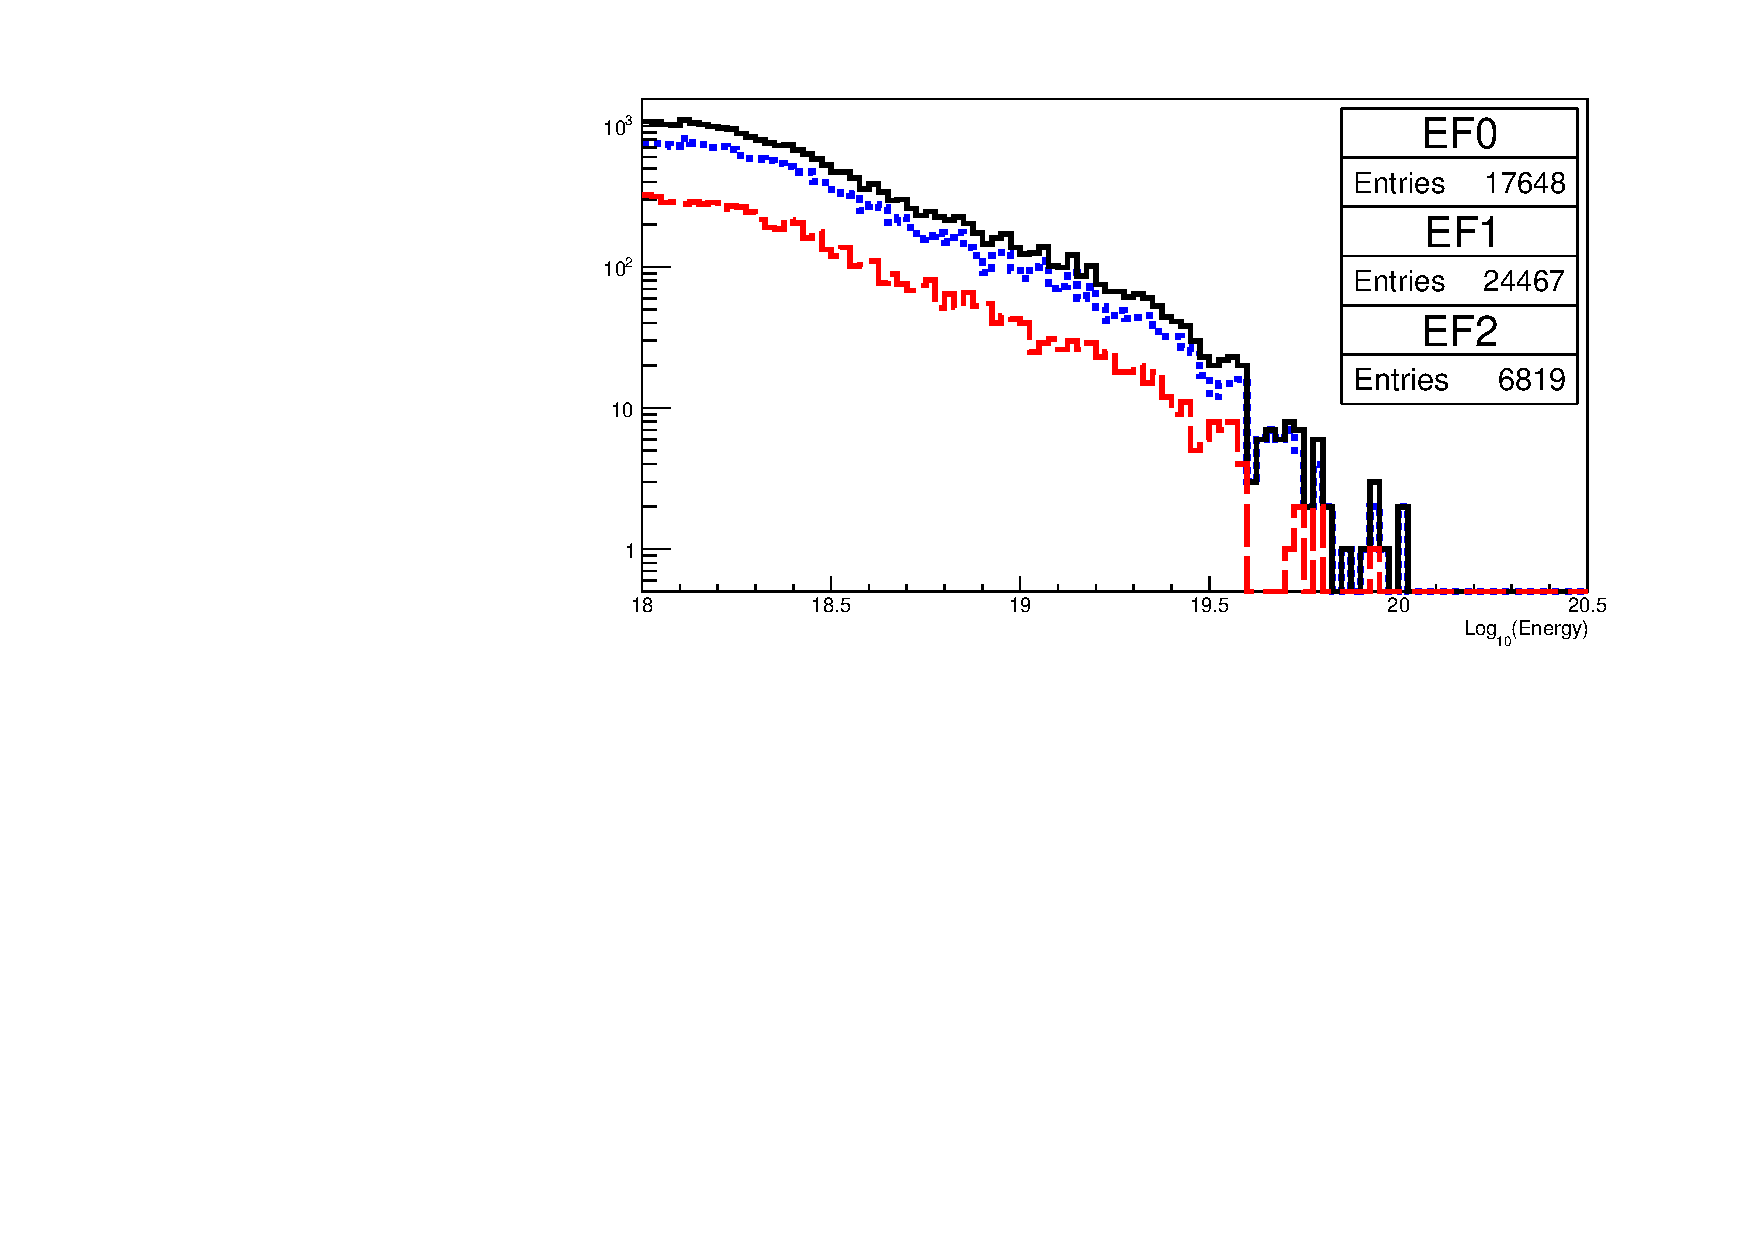
\includegraphics[width=\textwidth]{/home/tsudholz/PhD/Thesis/chapters/graphs/CloudFlags/EnergyHistAll_logE_18_0to20_5_Comb2.pdf}
\caption{Distribution of the energy of events within the bin of log(E) of 18.0 to 20.5. Black (EF1) denotes events that passed with the cloud cut removed, blue (EF0) denotes events that would pass the cloud cuts and red (EF2) denotes events that would fail the cloud cuts. All other cuts used for the ICRC19 have been applied.} \label{fig:cloudFlag_energyDist}
\end{figure}

%\begin{figure}
%\centering
%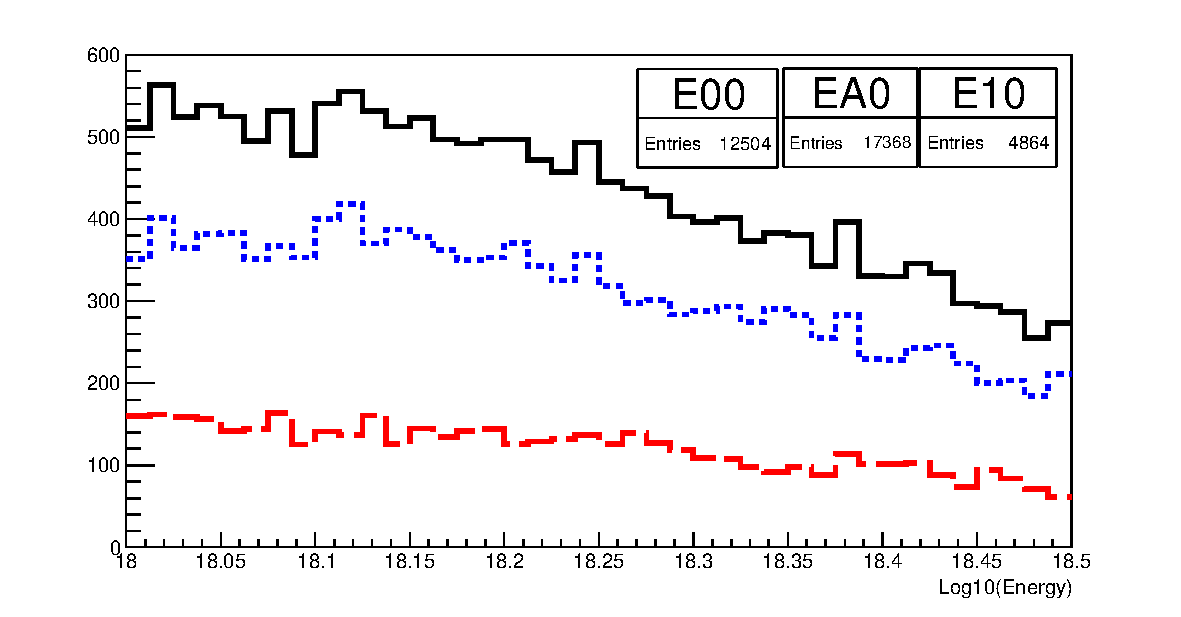
\includegraphics[width=\textwidth]{/home/tsudholz/PhD/Thesis/chapters/graphs/CloudFlags/EnergyHist_logE_18_0to18_5_Comb.pdf}
%\caption{Distribution of the energy of events within the bin of log(E) of 18.0 to 18.5. Black (EA0) denotes events that passed with cloud cut removed, blue (E00) denotes events that would pass the cloud cuts and red (E10) denotes events that would fail the cloud cuts. All other cuts used for the ICRC19 have been applied.}
%\end{figure}
%
%\begin{figure}
%\centering
%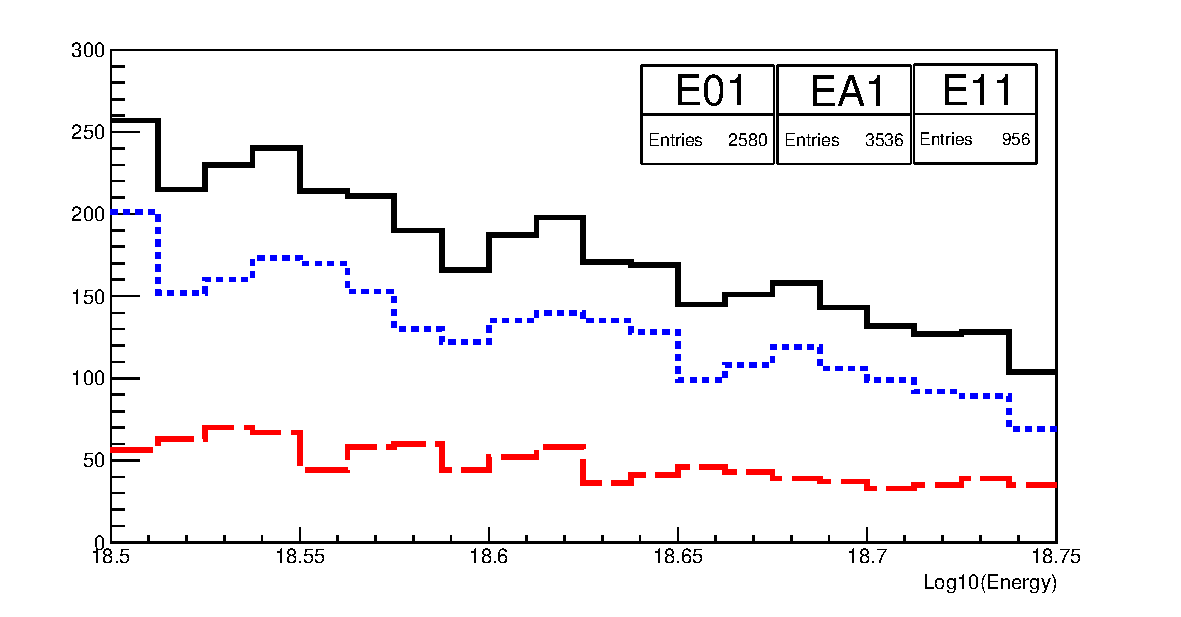
\includegraphics[width=\textwidth]{/home/tsudholz/PhD/Thesis/chapters/graphs/CloudFlags/EnergyHist_logE_18_5to18_75_Comb.pdf}
%\caption{Distribution of the energy of events within the bin of log(E) of 18.5 to 18.75. Black (EA1) denotes events that passed with cloud cut removed, blue (E01) denotes events that would pass the cloud cuts and red (E11) denotes events that would fail the cloud cuts. All other cuts used for the ICRC19 have been applied. }
%\end{figure}
%
%\begin{figure}
%\centering
%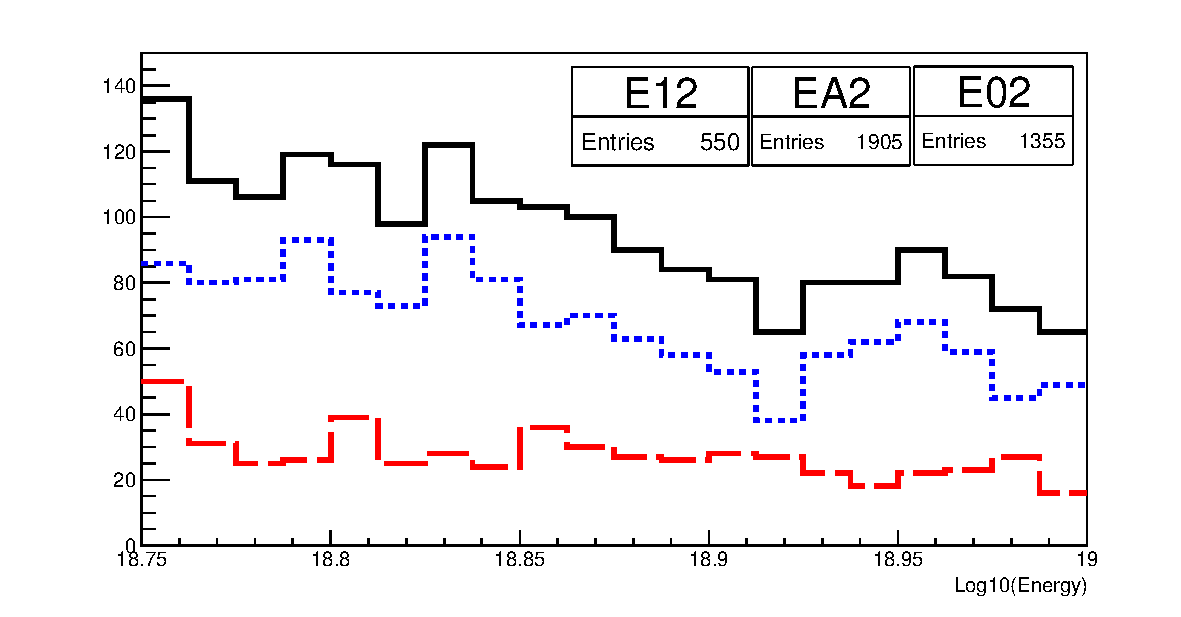
\includegraphics[width=\textwidth]{/home/tsudholz/PhD/Thesis/chapters/graphs/CloudFlags/EnergyHist_logE_18_75to19_0_Comb.pdf}
%\caption{Distribution of the energy of events within the bin of log(E) of 18.75 to 19.0. Black (EA2) denotes events that passed with cloud cut removed, blue (E12) denotes events that would pass the cloud cuts and red (E02) denotes events that would fail the cloud cuts. All other cuts used for the ICRC19 have been applied.}
%\end{figure}
%
%\begin{figure}
%\centering
%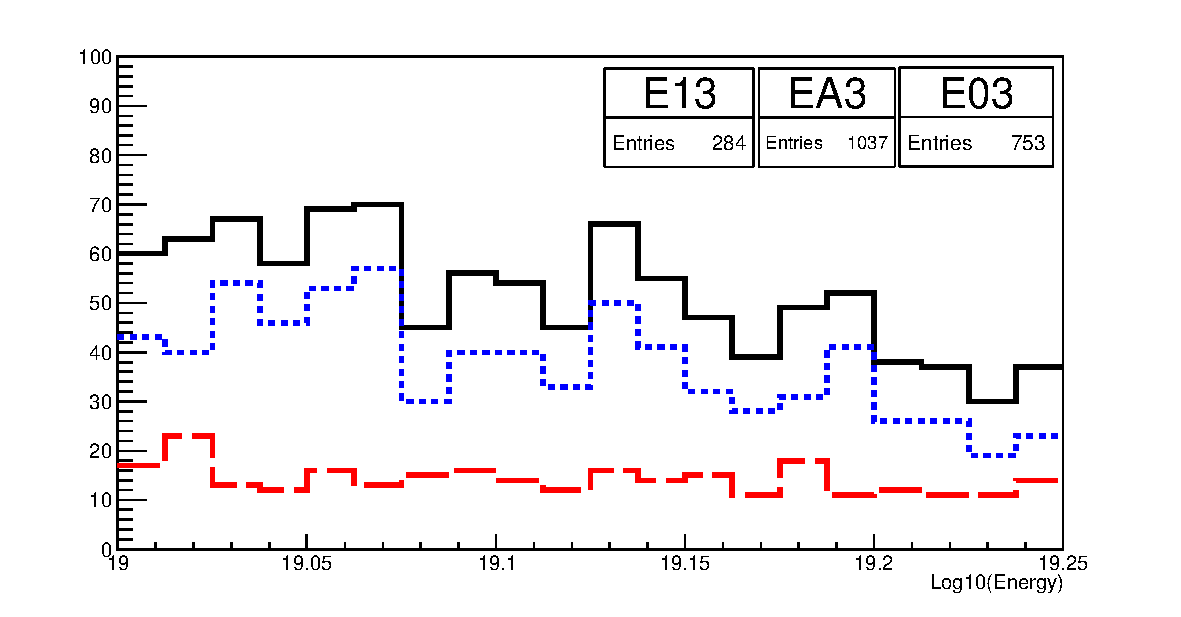
\includegraphics[width=\textwidth]{/home/tsudholz/PhD/Thesis/chapters/graphs/CloudFlags/EnergyHist_logE_19_0to19_25_Comb.pdf}
%\caption{Distribution of the energy of events within the bin of log(E) of 19.0 to 19.25. Black (EA3) denotes events that passed with cloud cut removed, blue (E13) denotes events that would pass the cloud cuts and red (E03) denotes events that would fail the cloud cuts. All other cuts used for the ICRC19 have been applied.}
%\end{figure}
%
%\begin{figure}
%\centering
%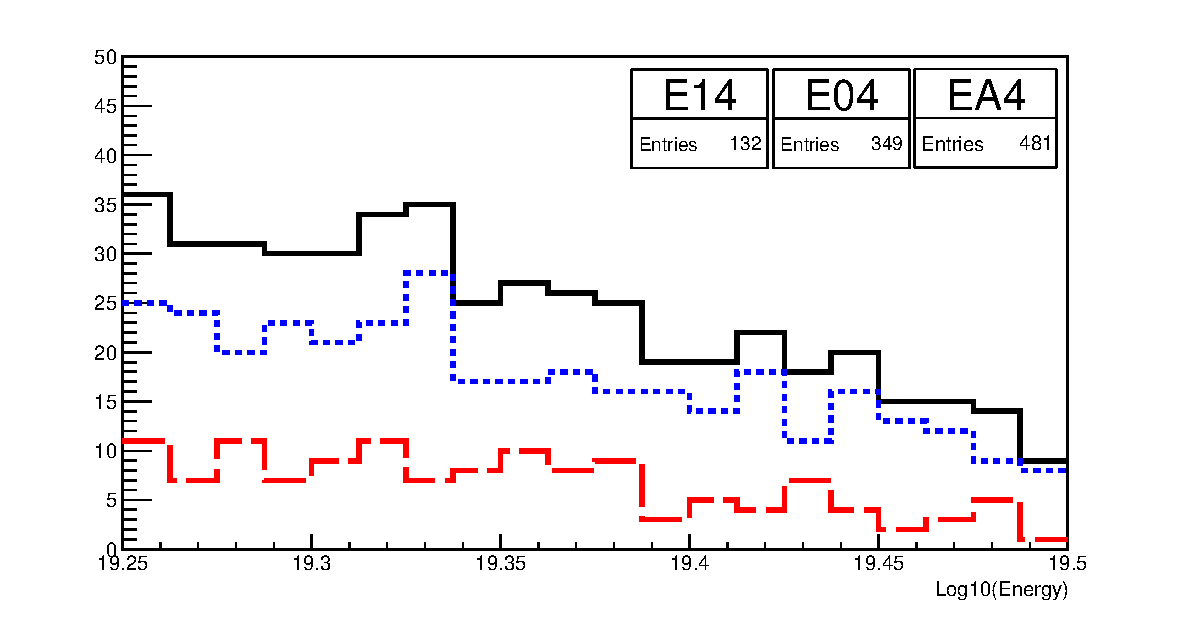
\includegraphics[width=\textwidth]{/home/tsudholz/PhD/Thesis/chapters/graphs/CloudFlags/EnergyHist_logE_19_25to19_5_Comb.pdf}
%\caption{Distribution of the energy of events within the bin of log(E) of 19.25 to 19.5. Black (EA4) denotes events that passed with cloud cut removed, blue (E14) denotes events that would pass the cloud cuts and red (E04) denotes events that would fail the cloud cuts. All other cuts used for the ICRC19 have been applied.}
%\end{figure}
%
%\begin{figure}
%\centering
%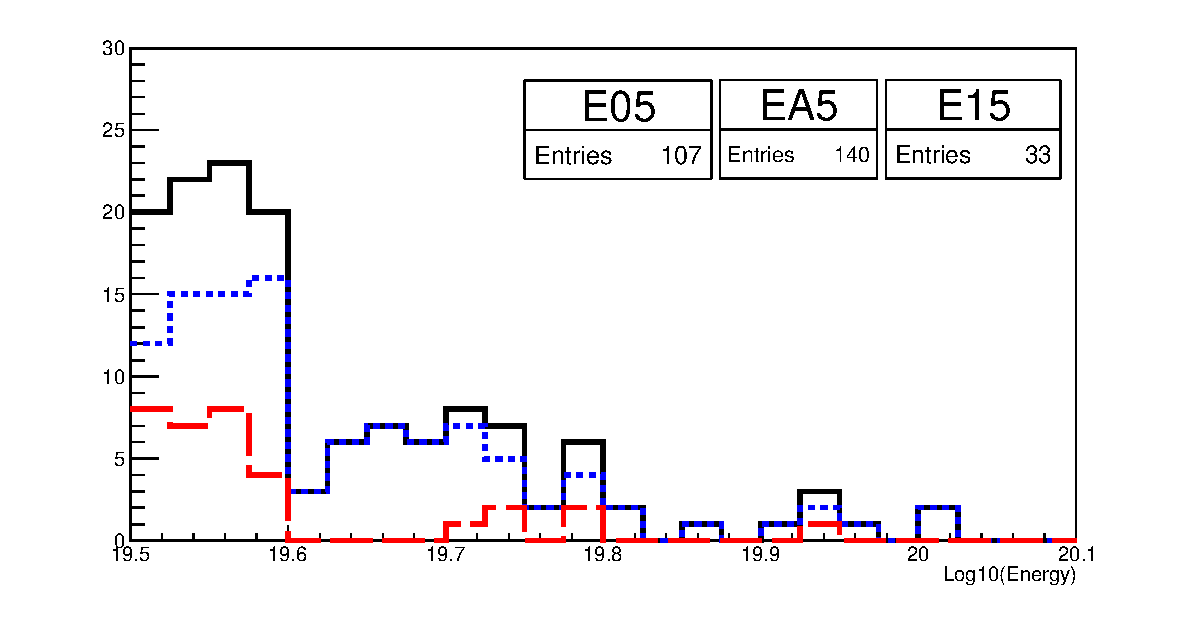
\includegraphics[width=\textwidth]{/home/tsudholz/PhD/Thesis/chapters/graphs/CloudFlags/EnergyHist_logE_Greater19_5_Comb.pdf}
%\caption{Distribution of the energy of events within the bin of log(E) of greater than 19.5. Black (EA5) denotes events that passed with cloud cut removed, blue (E15) denotes events that would pass the cloud cuts and red (E05) denotes events that would fail the cloud cuts. All other cuts used for the ICRC19 have been applied.}
%\end{figure}

% Xmax Distribution for Passed, Combined, Failed

\subsection{Xmax Distribution}




\begin{figure}[!p]
\centering
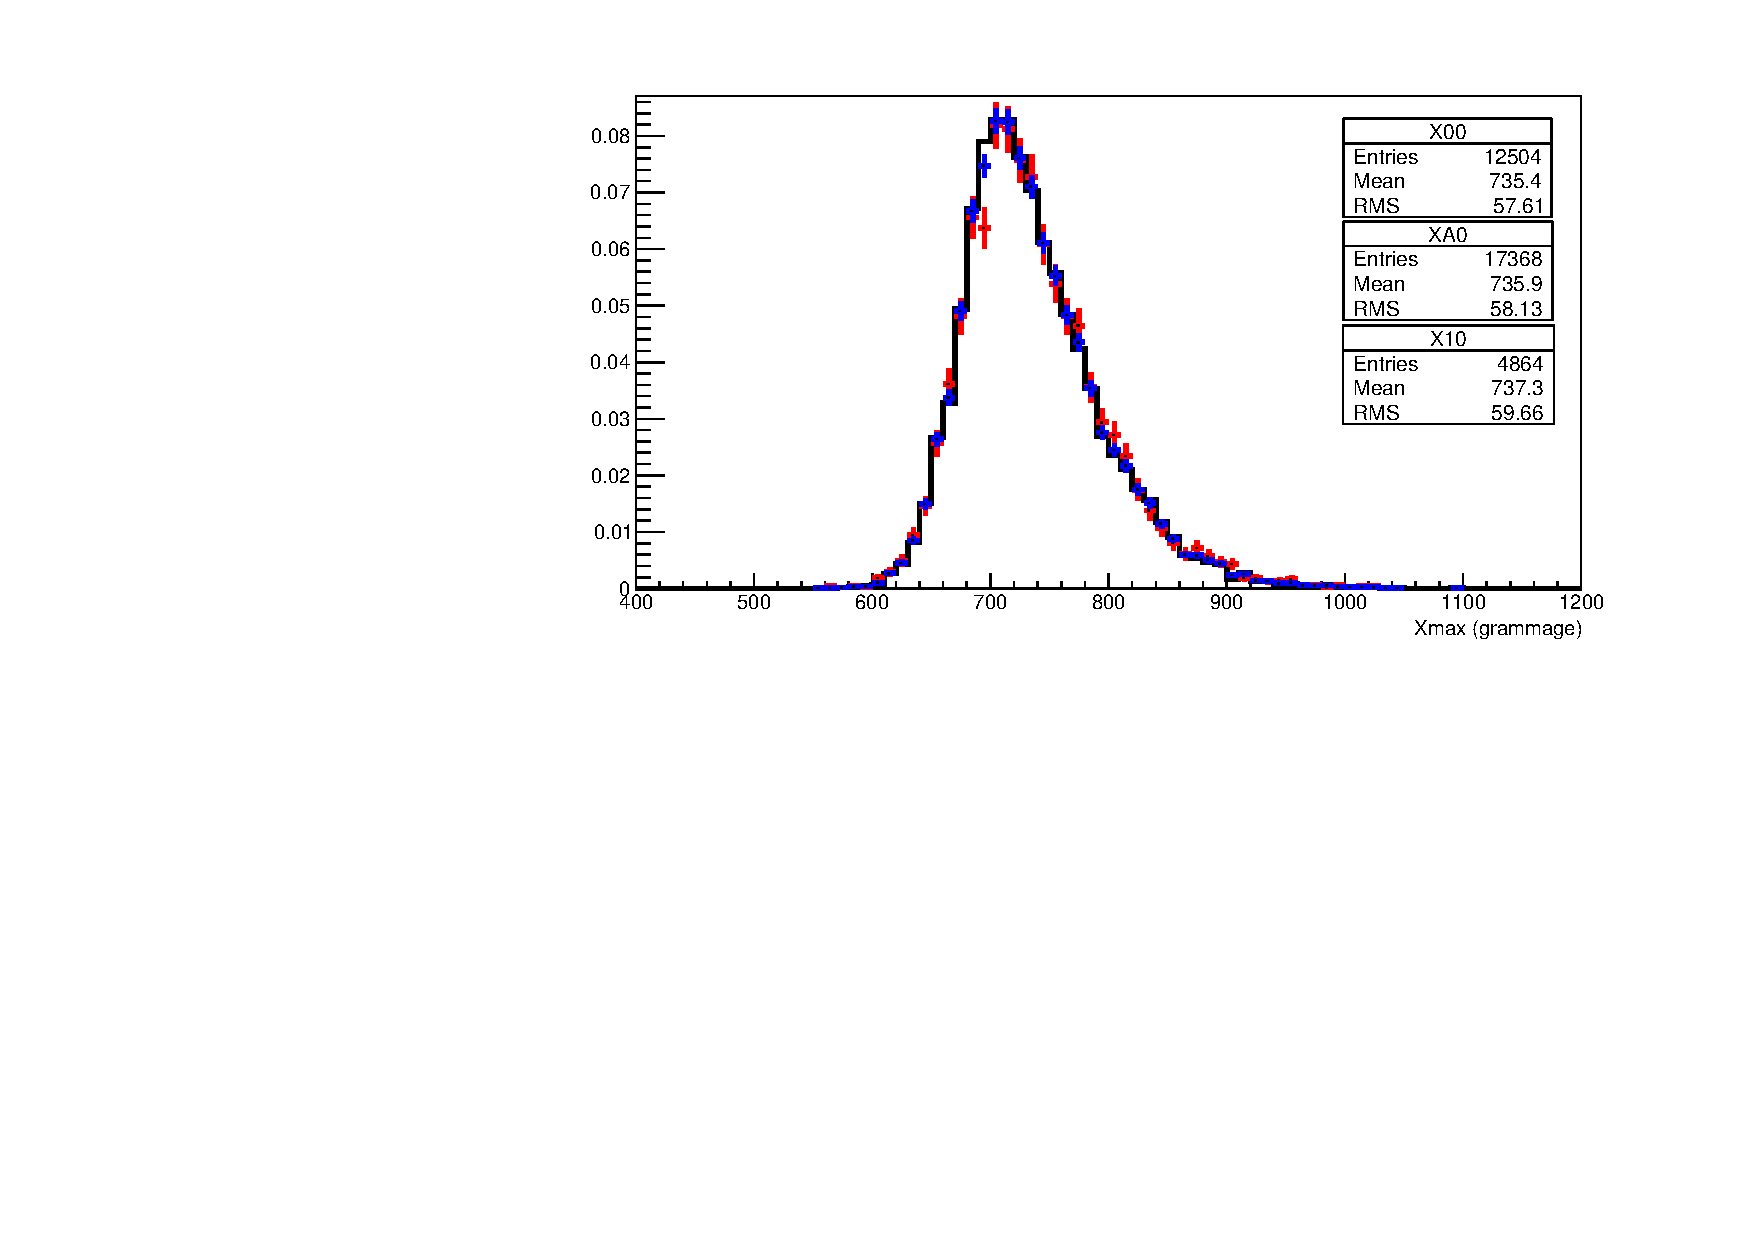
\includegraphics[width=\textwidth]{/home/tsudholz/PhD/Thesis/chapters/graphs/CloudFlags/NormHist_Xmax_logE_18_0to18_5_Comb.pdf}
\caption{Distribution of the Xmax of events within the bin of log(E) of 18.0 to 18.5. Black (XA0) denotes events that passed with cloud cut removed, blue (X00) denotes events that would pass the cloud cuts and red (X10) denotes events that would fail the cloud cuts. All other cuts used for the ICRC19 have been applied.} \label{fig:CloudFlag_XmaxDist_18.0}
\end{figure}

\begin{figure}[!p]
\centering
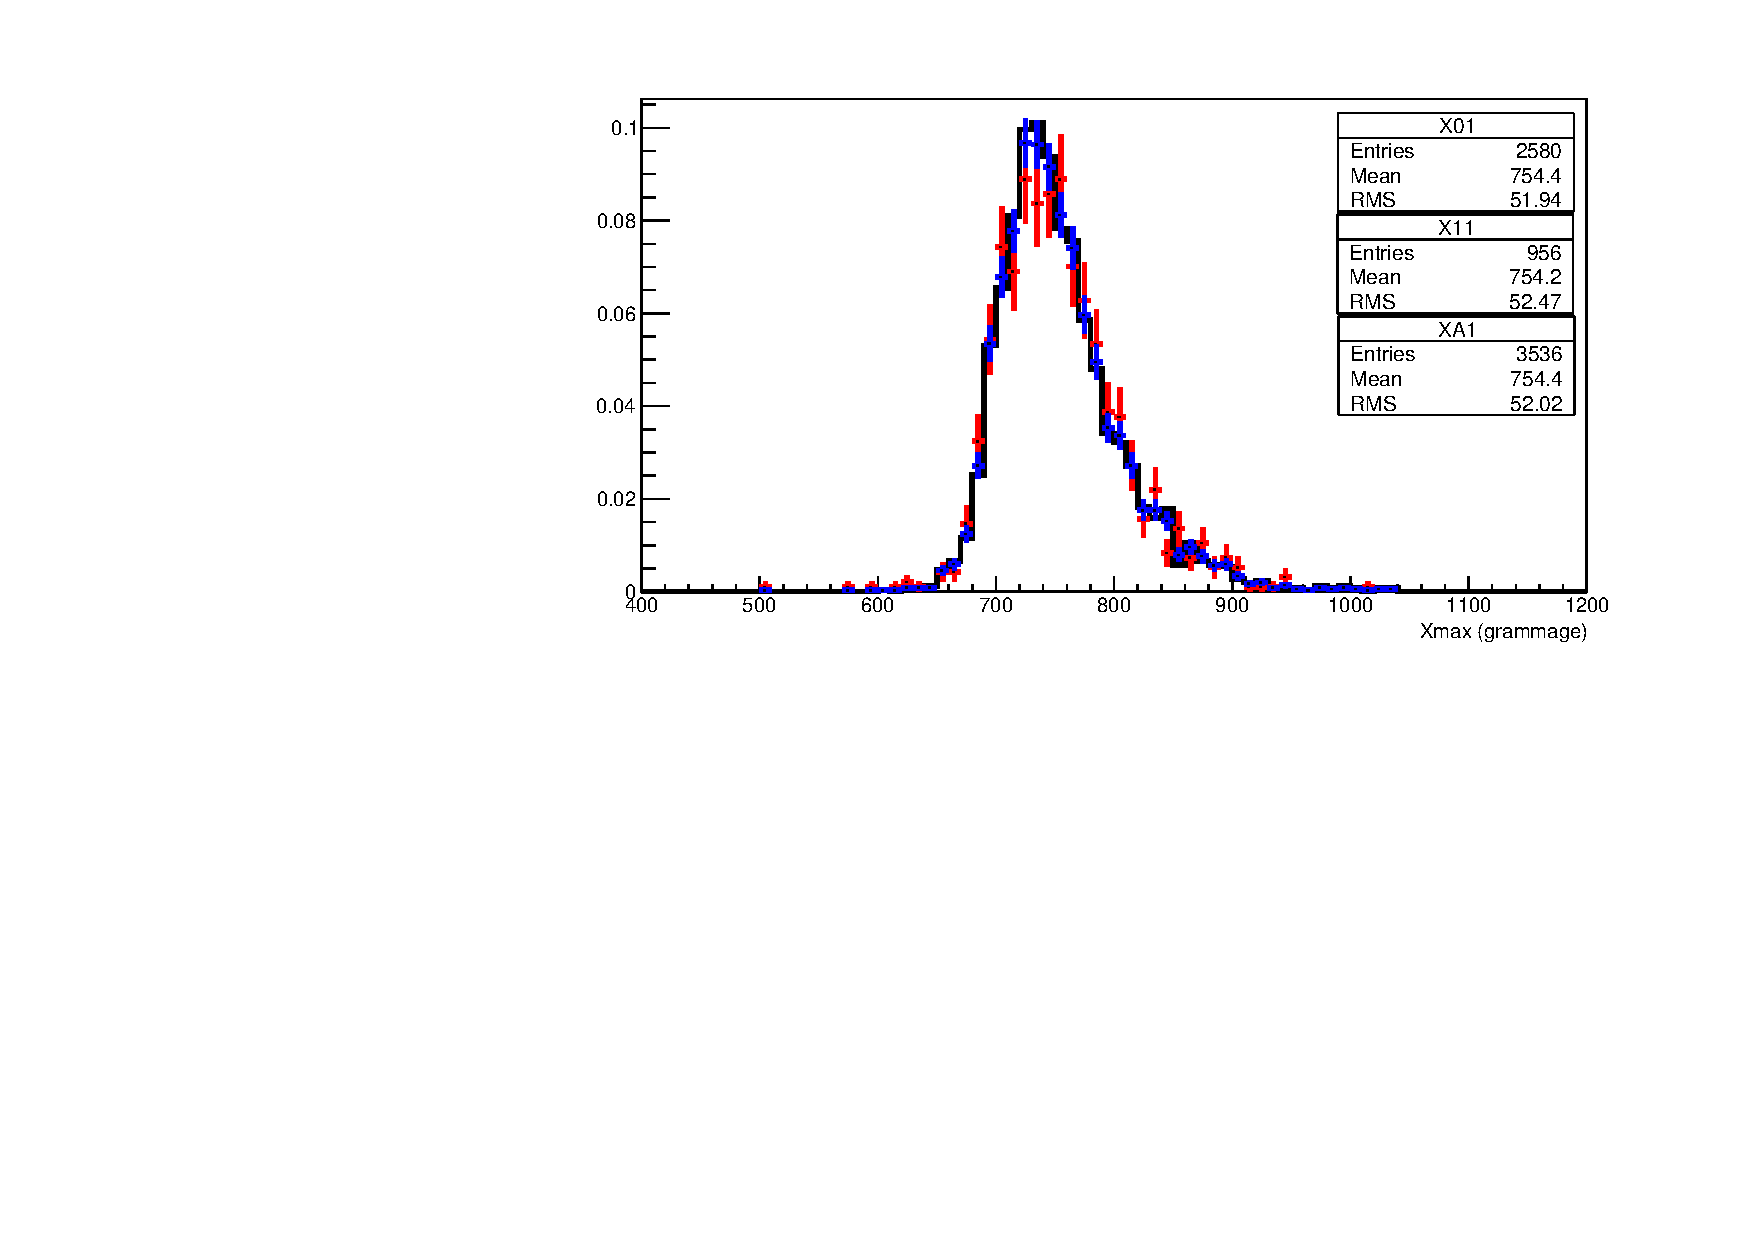
\includegraphics[width=\textwidth]{/home/tsudholz/PhD/Thesis/chapters/graphs/CloudFlags/NormHist_Xmax_logE_18_5to18_75_Comb.pdf}
\caption{Distribution of the Xmax of events within the bin of log(E) of 18.5 to 18.75. Black (XA1) denotes events that passed with cloud cut removed, blue (X01) denotes events that would pass the cloud cuts and red (X11) denotes events that would fail the cloud cuts. All other cuts used for the ICRC19 have been applied.}\label{fig:CloudFlag_XmaxDist_18.5}
\end{figure}

\begin{figure}[!p]
\centering
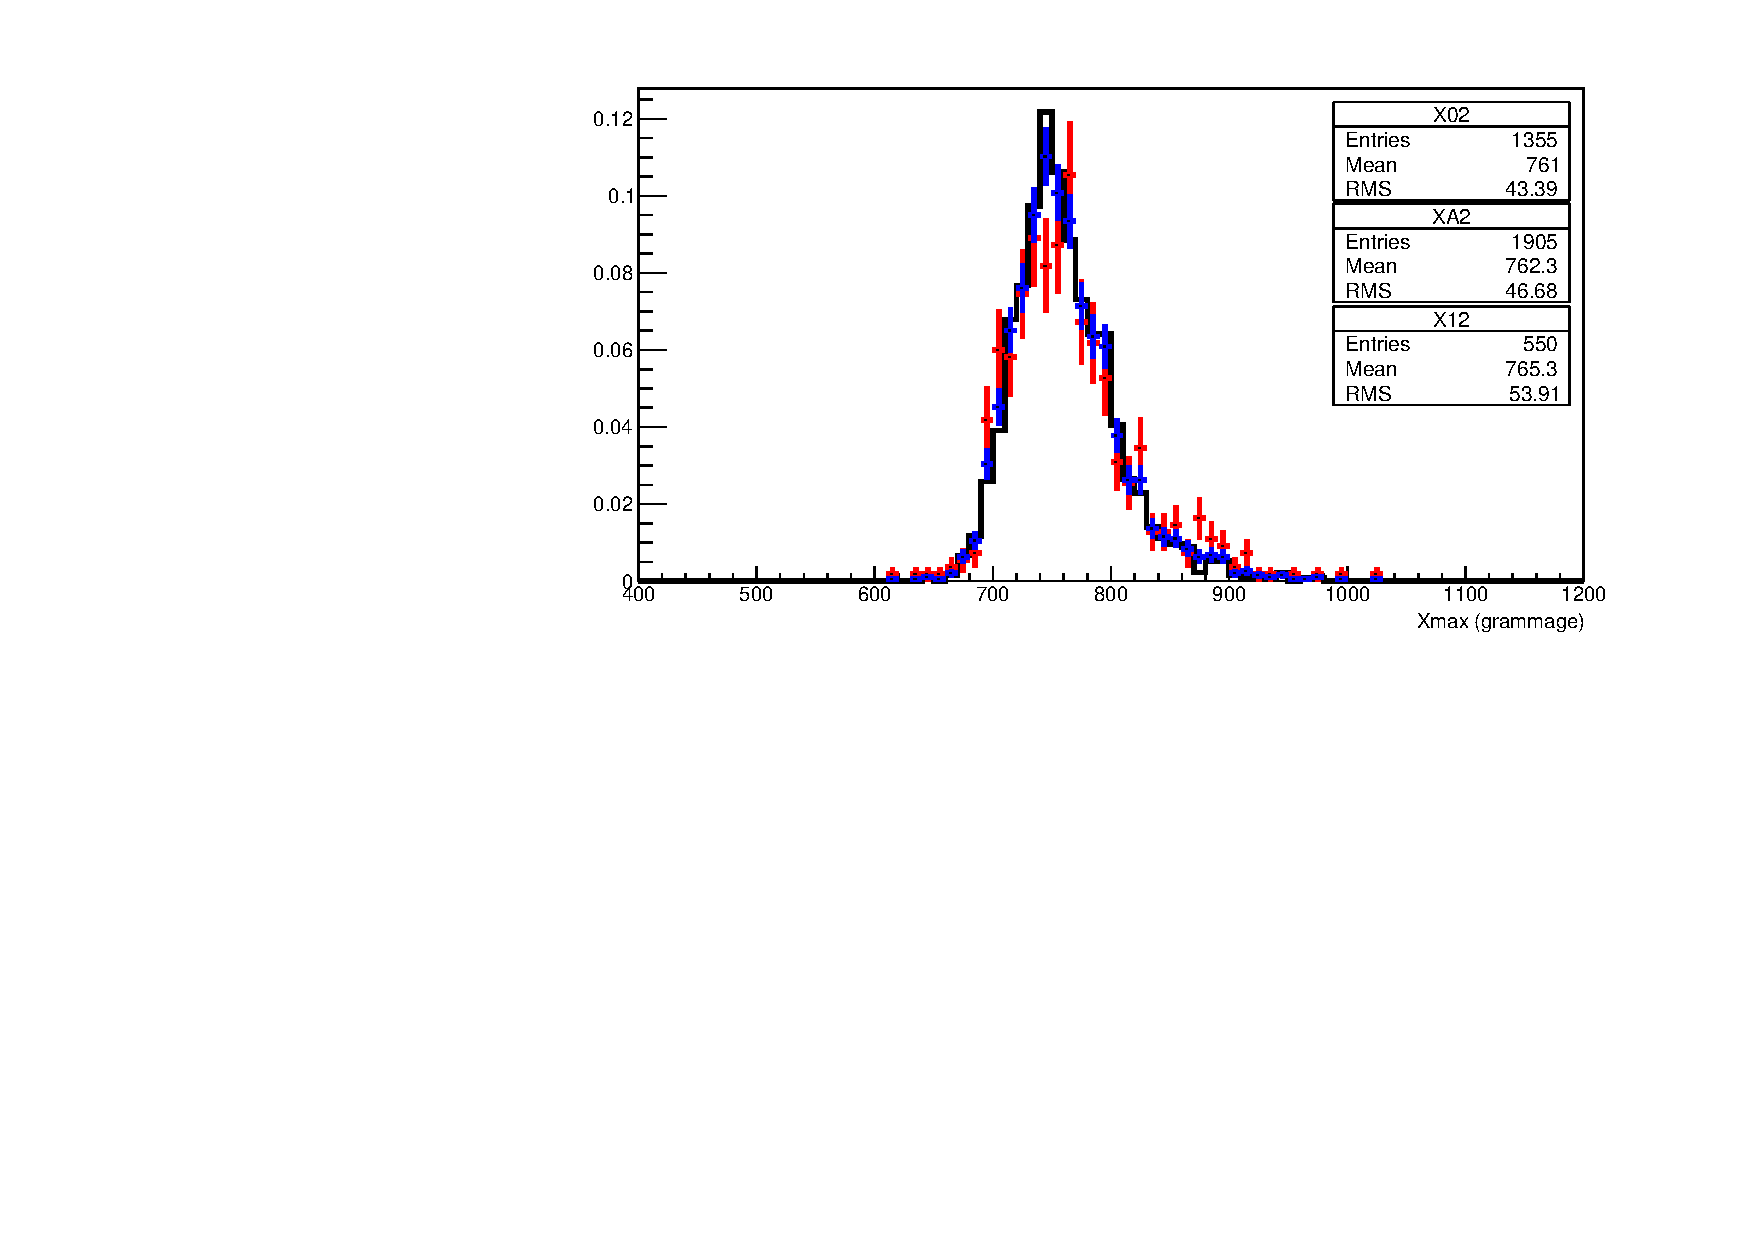
\includegraphics[width=\textwidth]{/home/tsudholz/PhD/Thesis/chapters/graphs/CloudFlags/NormHist_Xmax_logE_18_75to19_0_Comb.pdf}
\caption{Distribution of the Xmax of events within the bin of log(E) of 19.0 to 19.25. Black (XA2) denotes events that passed with cloud cut removed, blue (X02) denotes events that would pass the cloud cuts and red (X12) denotes events that would fail the cloud cuts. All other cuts used for the ICRC19 have been applied.}\label{fig:CloudFlag_XmaxDist_18.75}
\end{figure}

\begin{figure}[!p]
\centering
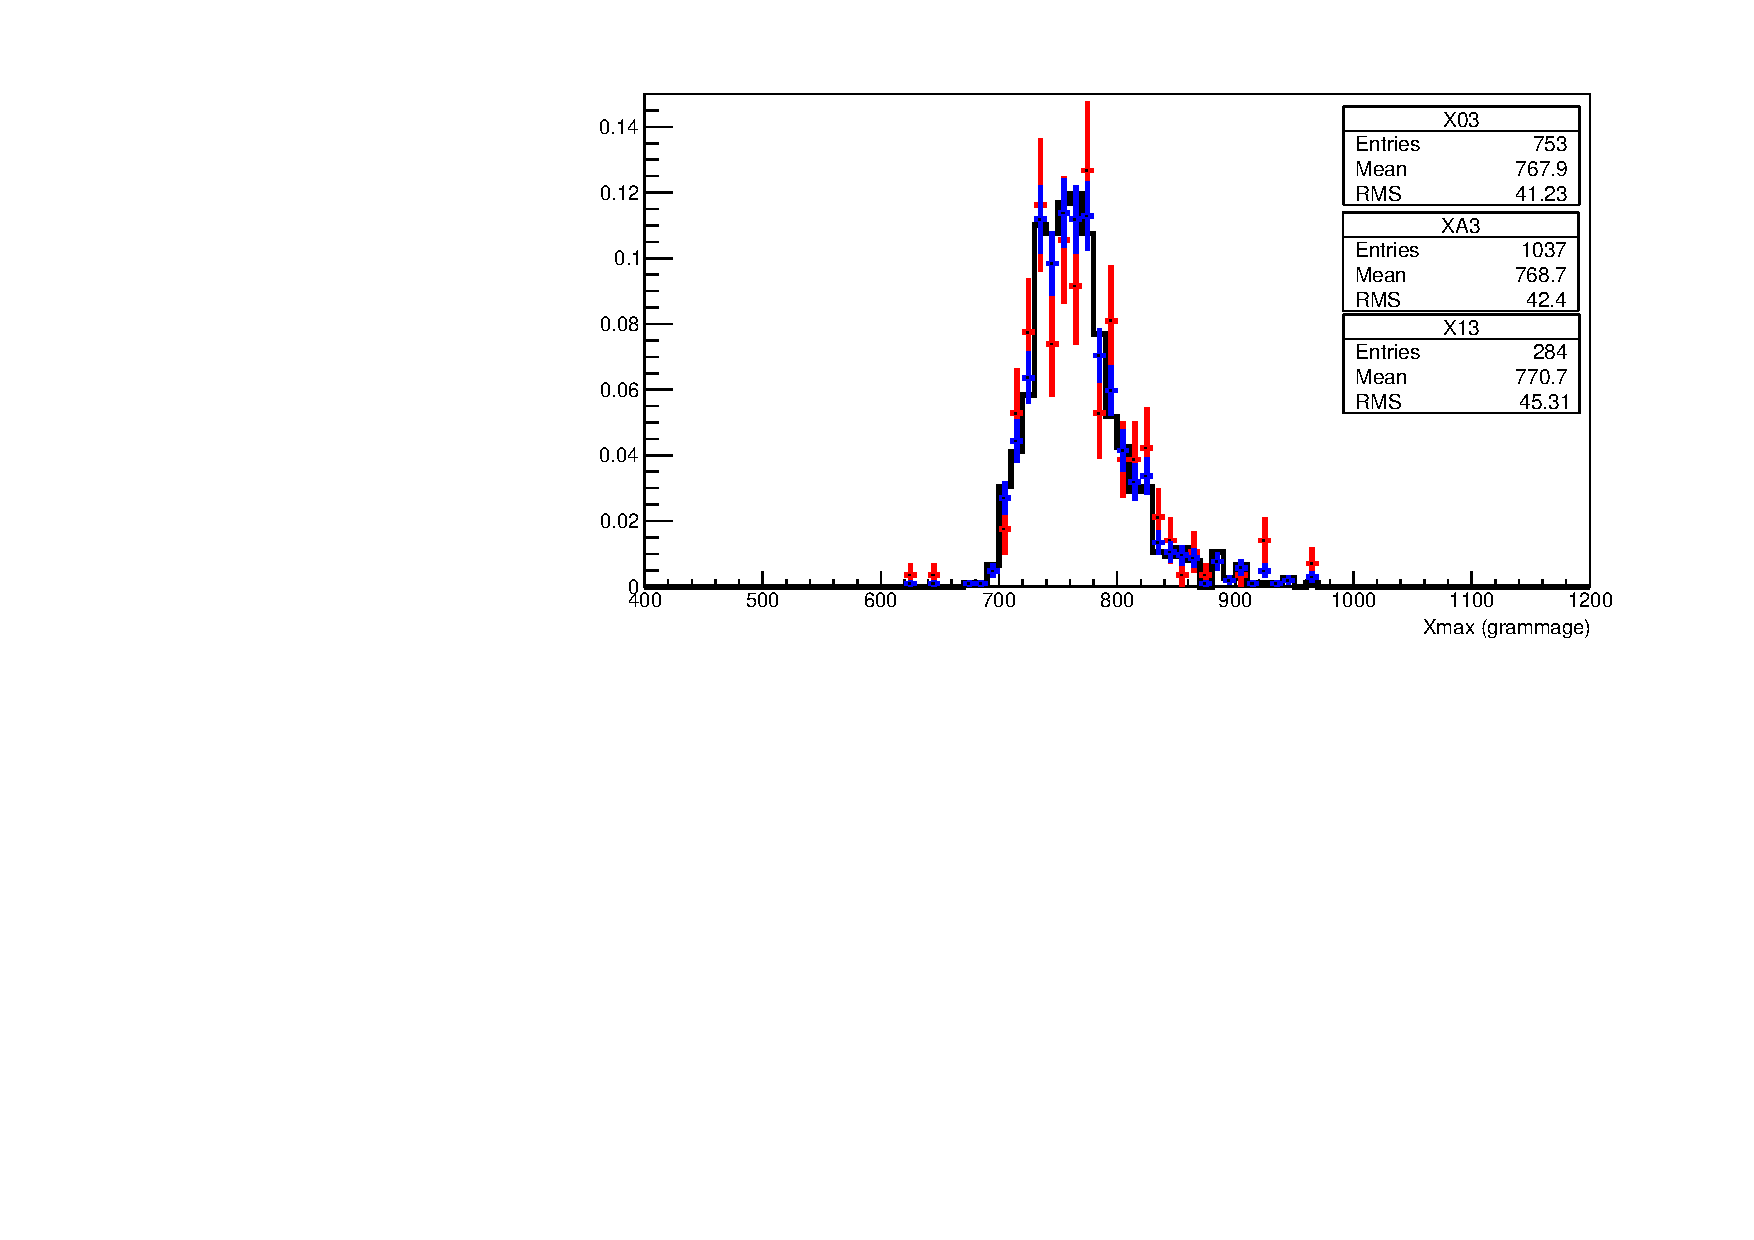
\includegraphics[width=\textwidth]{/home/tsudholz/PhD/Thesis/chapters/graphs/CloudFlags/NormHist_Xmax_logE_19_0to19_25_Comb.pdf}
\caption{Distribution of the Xmax of events within the bin of log(E) of 19.0 to 19.25. Black (XA3) denotes events that passed with cloud cut removed, blue (X03) denotes events that would pass the cloud cuts and red (X13) denotes events that would fail the cloud cuts. All other cuts used for the ICRC19 have been applied.}\label{fig:CloudFlag_XmaxDist_19.0}
\end{figure}

\begin{figure}[!p]
\centering
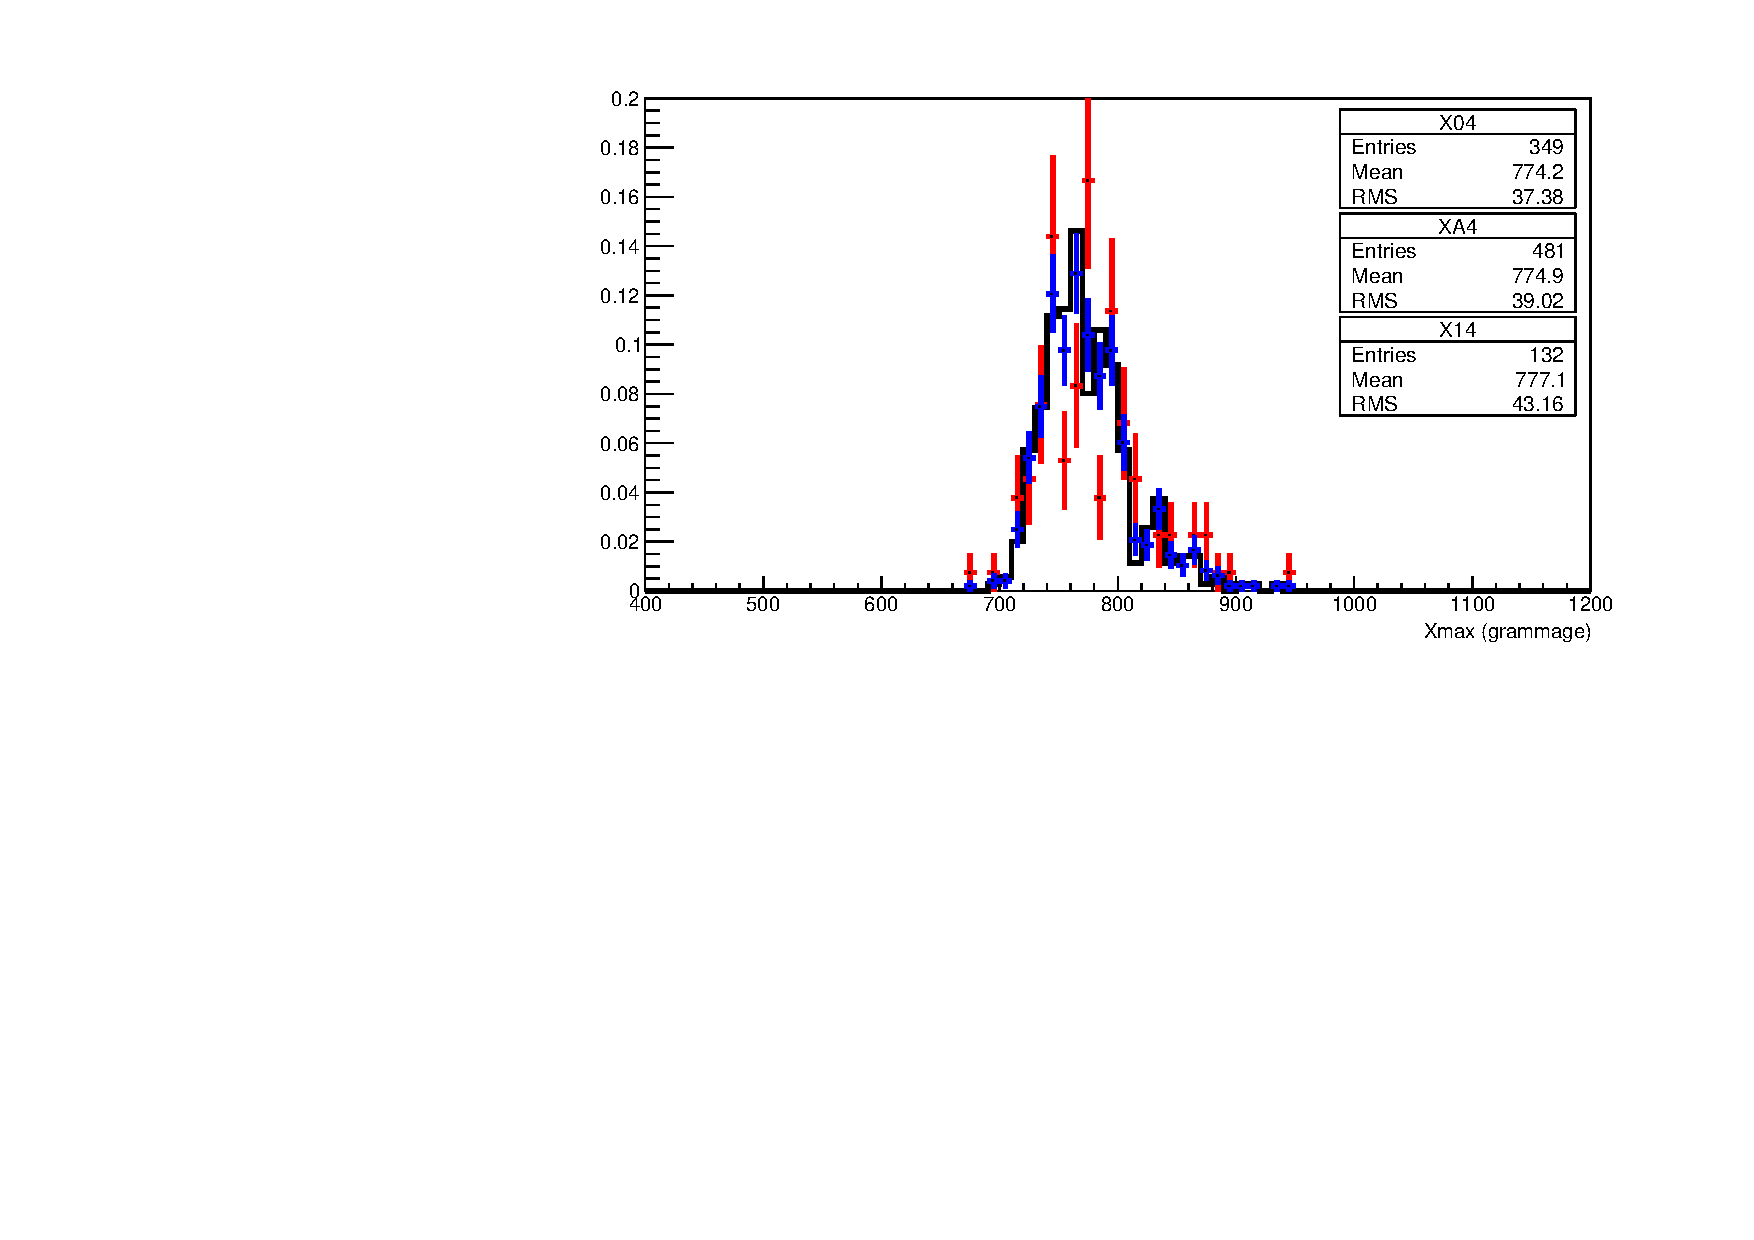
\includegraphics[width=\textwidth]{/home/tsudholz/PhD/Thesis/chapters/graphs/CloudFlags/NormHist_Xmax_logE_19_25to19_5_Comb.pdf}
\caption{Distribution of the Xmax of events within the bin of log(E) of 19.25 to 19.5. Black (XA4) denotes events that passed with cloud cut removed, blue (X04) denotes events that would pass the cloud cuts and red (X14) denotes events that would fail the cloud cuts. All other cuts used for the ICRC19 have been applied.}\label{fig:CloudFlag_XmaxDist_19.25}
\end{figure}

\begin{figure}[!p]
\centering
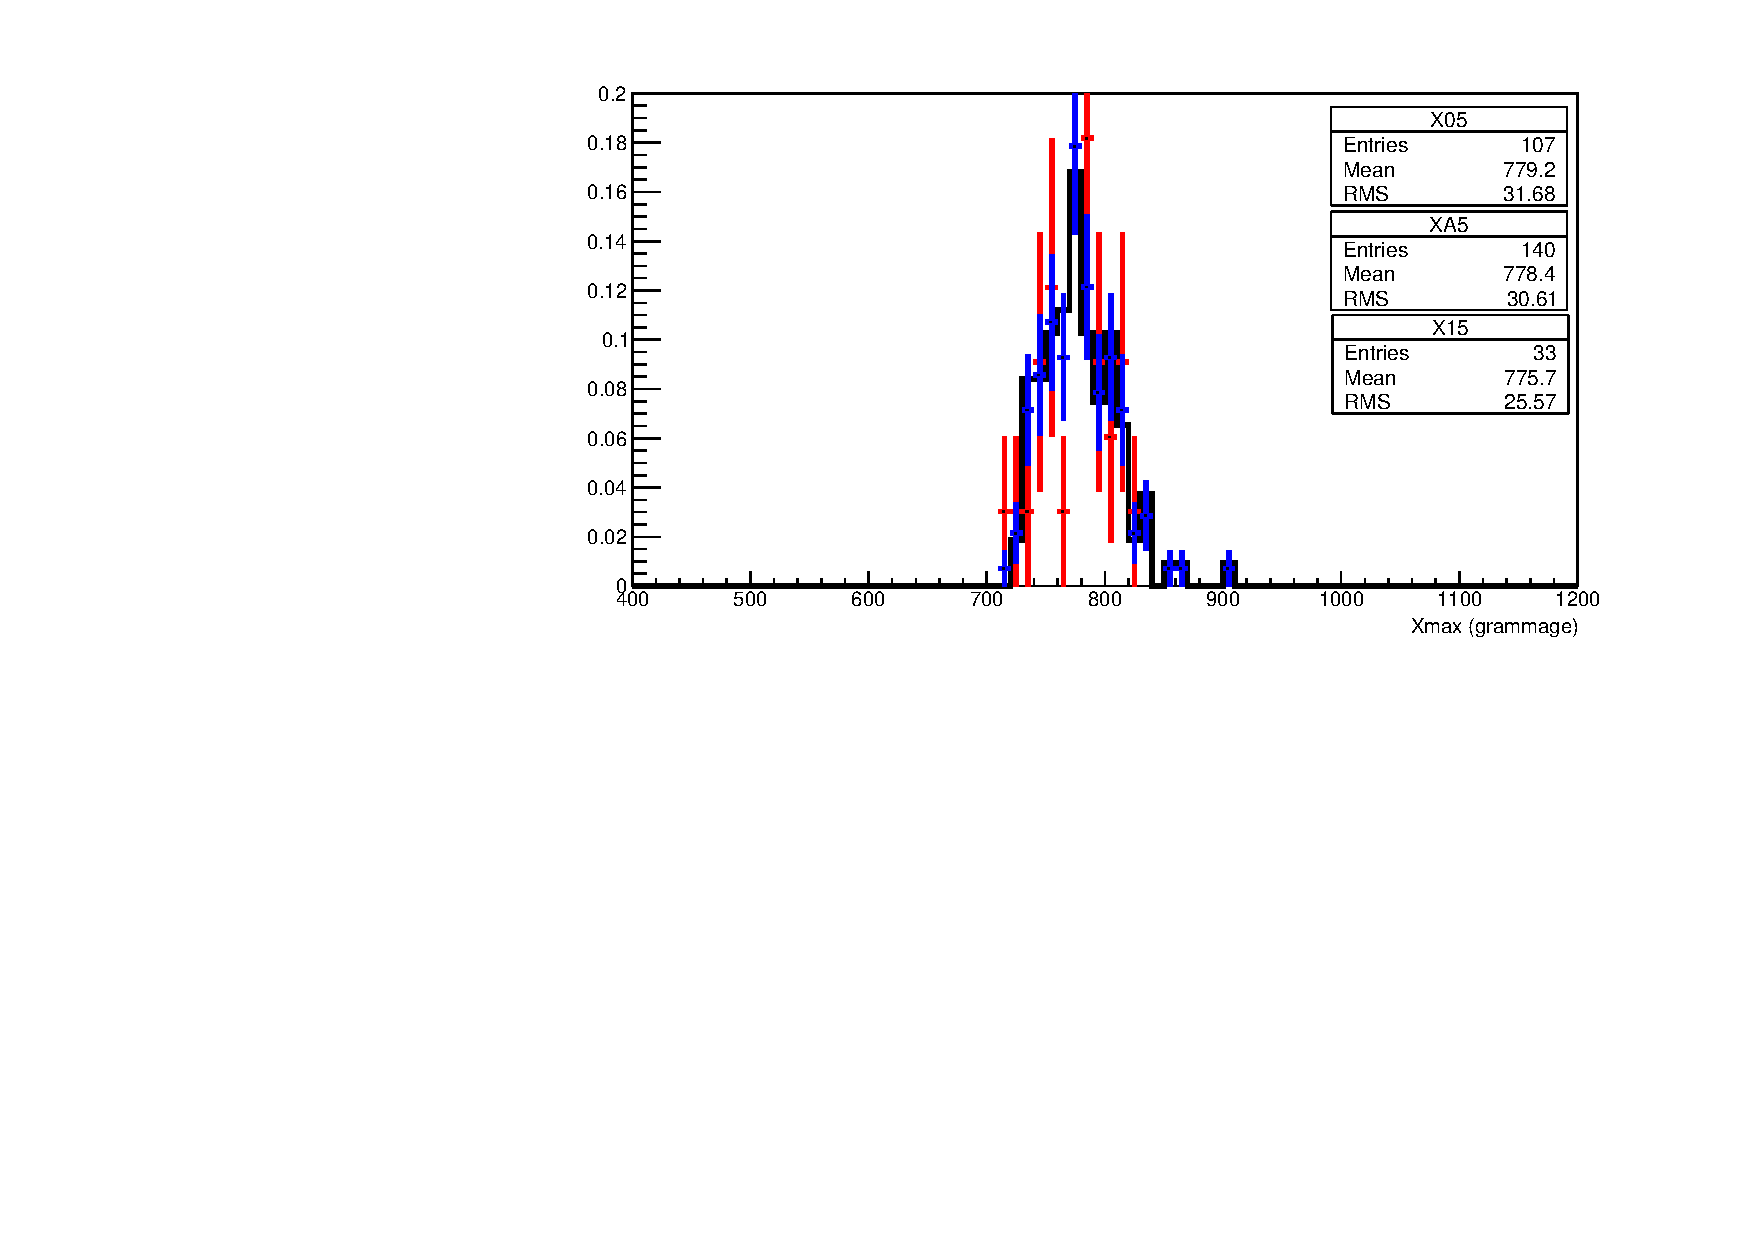
\includegraphics[width=\textwidth]{/home/tsudholz/PhD/Thesis/chapters/graphs/CloudFlags/NormHist_Xmax_logE_Greater19_5_Comb.pdf}
\caption{Distribution of the Xmax of events within the bin of log(E) of greater than 19.5. Black (XA5) denotes events that passed with cloud cut removed, blue (X05) denotes events that would pass the cloud cuts and red (X15) denotes events that would fail the cloud cuts. All other cuts used for the ICRC19 have been applied.}\label{fig:CloudFlag_XmaxDist_19.5}
\end{figure}

Comparison of Xmax distributions between data sets with the cloud cut, without the cloud cut and a data set that just contains events that would fail the cloud cut. Each of these distributions has been normalised as each distribution has different amounts and it allows the shape to be more easily compared. The dataset is split into six log$_{10}$(energy) bins to show the Xmax distribution: 18.0 to 18.5, 18.5 to 18.75, 18.75 to 19.0, 19.0 to 19.25, 19.25 to 19.5 and greater than 19.5. From looking at the mean and standard deviations each of the distributions are not significantly different. From Figure \ref{fig:CloudFlag_XmaxDist_18.0} to Figure \ref{fig:CloudFlag_XmaxDist_19.5} the black continuous line denotes all events that pass just the quality cuts with the cloud cuts removed, blurs points denote the events that would pass all the quality cuts including the cloud cuts and red denotes events that would pass all the quality cuts except for the cloud cuts.

Adding the rejected events back into the distribution allows the number of events to increase by around 30\%. This is a great addition to the highest energy bin (in this case $>$ 10$^{19.5}$ eV) where the statistics are low.

% Xmax Distribution for Failed only

\subsection{Xmax Distribution for Events that Failed Cloud Cut}



\begin{figure}[!p]
\centering
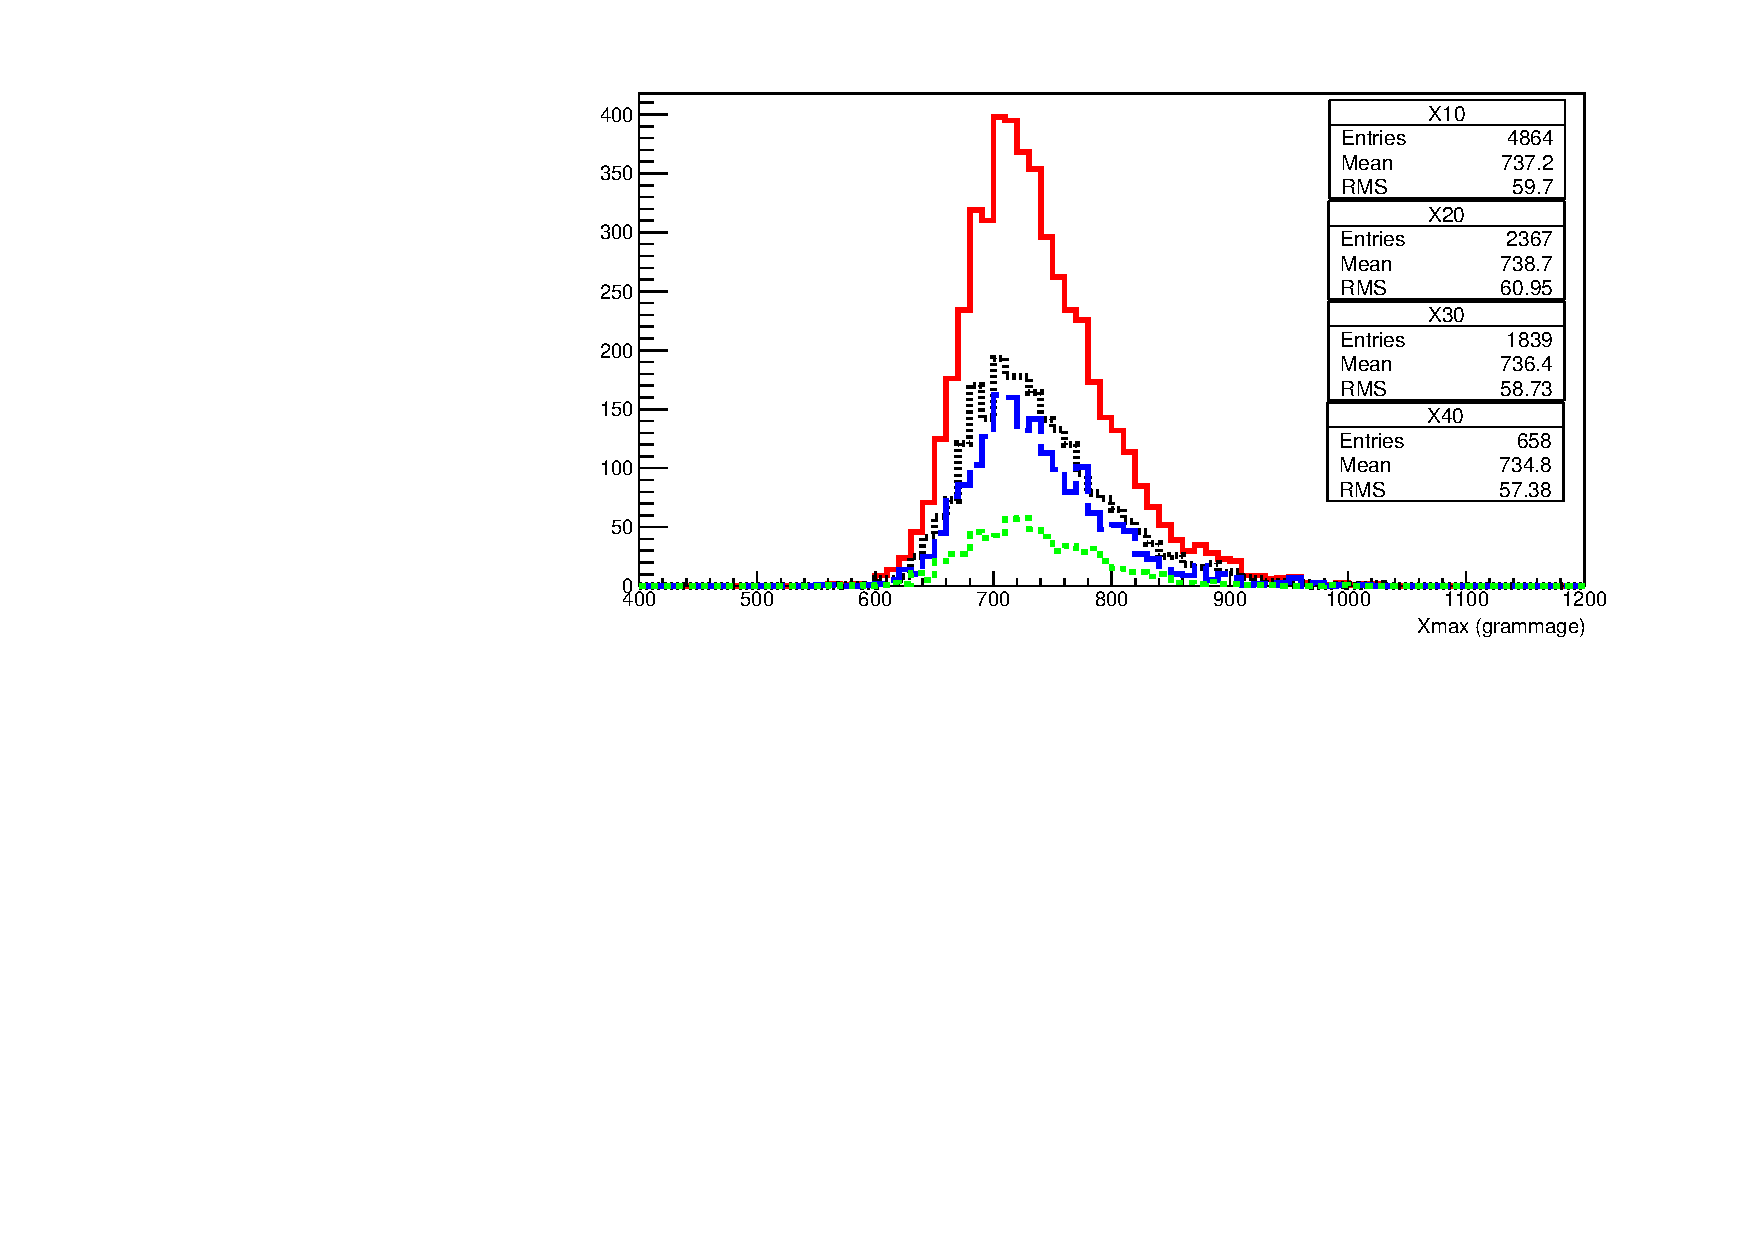
\includegraphics[width=\textwidth]{/home/tsudholz/PhD/Thesis/chapters/graphs/CloudFlags/NormHist_Xmax_FailedCloudCut_logE_18_0to18_5_Comb.pdf}
\caption{Distribution of the energy of events within the bin of log(E) of 18.0 to 18.5. Red (X10) denotes all event that failed the cloud cuts, black (X20) denotes events that failed the cloud camera/lidar cut, blue (X30) denotes events that failed the GOES data cut and green (X40) are events that have fail a combination of CLF/XLF, GOES and Cloud camera cut.} \label{fig:CloudFlag_XmaxFailed_18.0}
\end{figure}

\begin{figure}[!p]
\centering
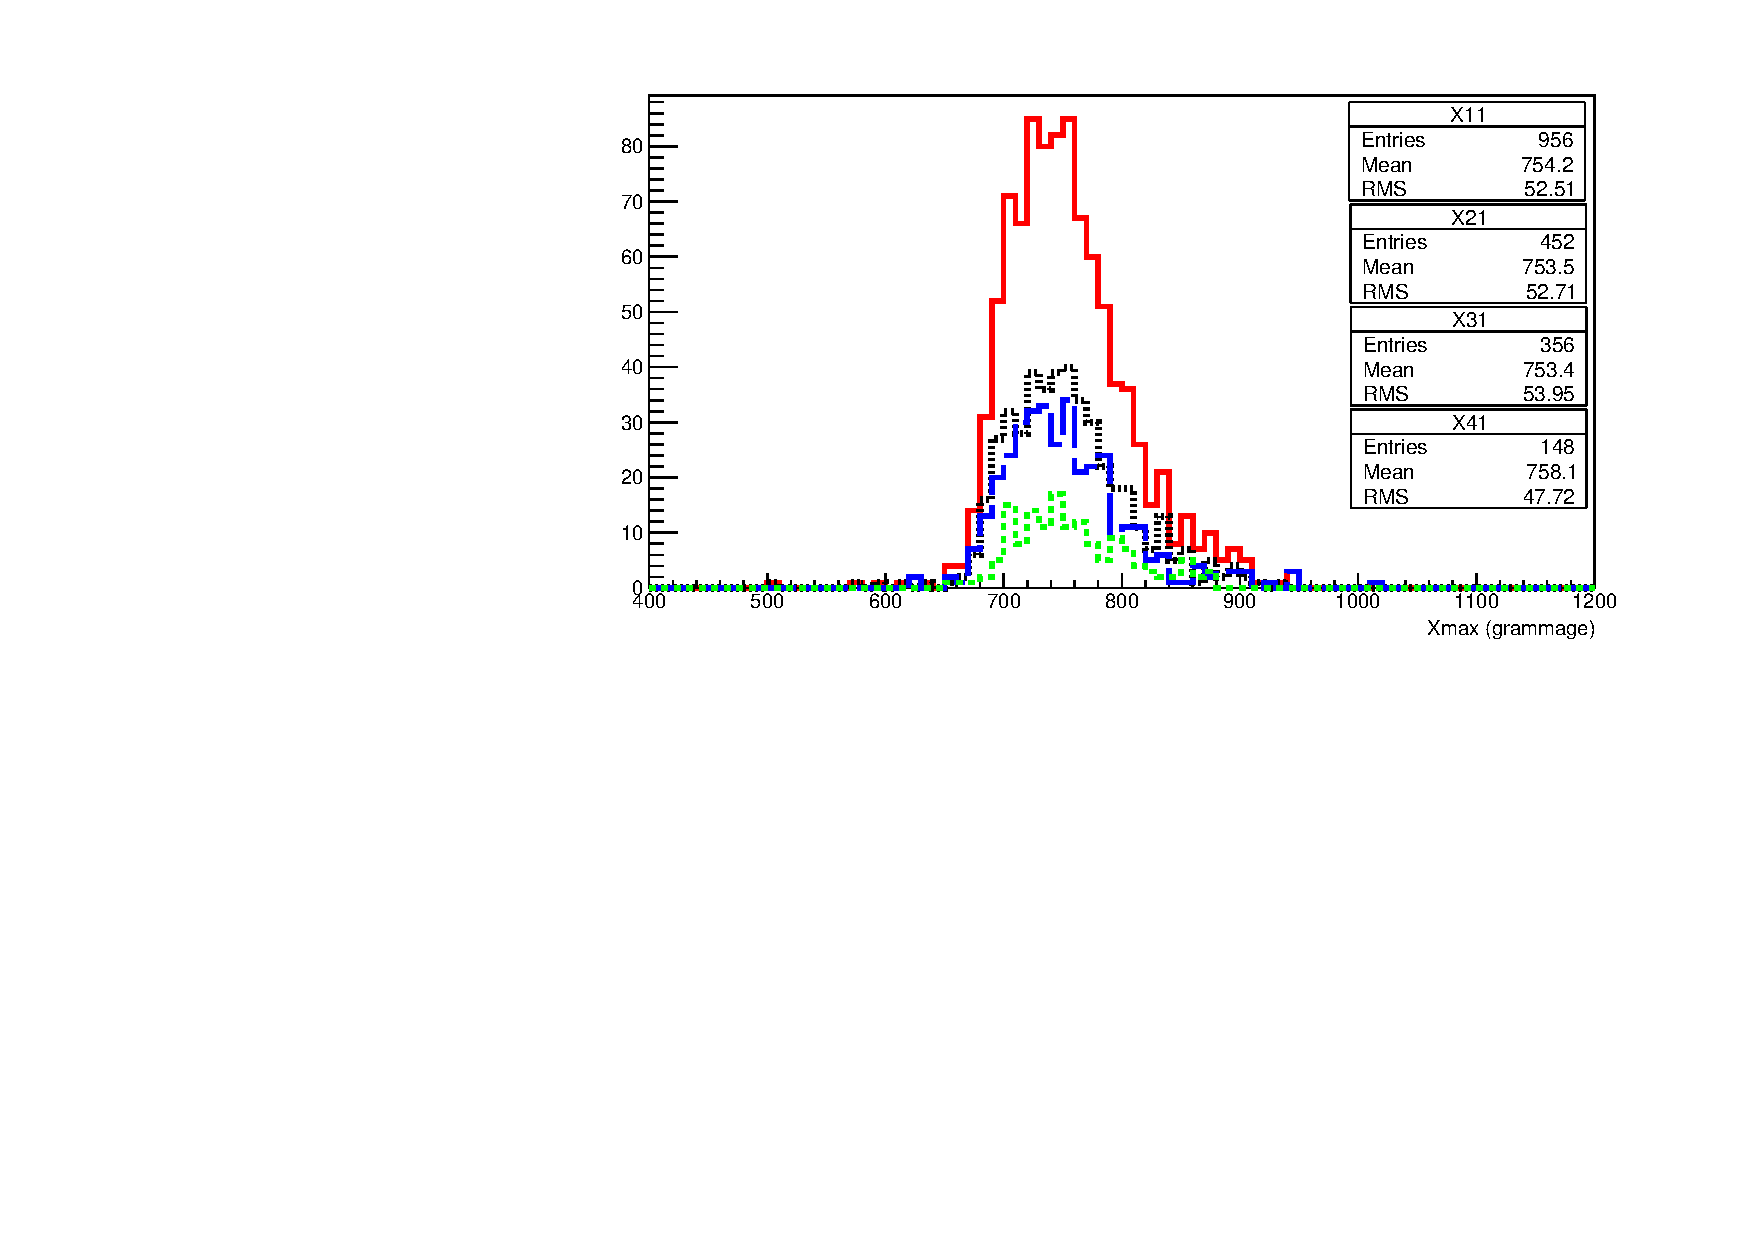
\includegraphics[width=\textwidth]{/home/tsudholz/PhD/Thesis/chapters/graphs/CloudFlags/NormHist_Xmax_FailedCloudCut_logE_18_5to18_75_Comb.pdf}
\caption{Distribution of the energy of events within the bin of log(E) of 18.5 to 18.75. Red (X11) denotes all event that failed the cloud cuts, black (X21) denotes events that failed the cloud camera/lidar cut, blue (X31) denotes events that failed the GOES data cut and green (X41) are events that have fail a combination of CLF/XLF, GOES and Cloud camera cut.} \label{fig:CloudFlag_XmaxFailed_18.5}
\end{figure}

\begin{figure}[!p]
\centering
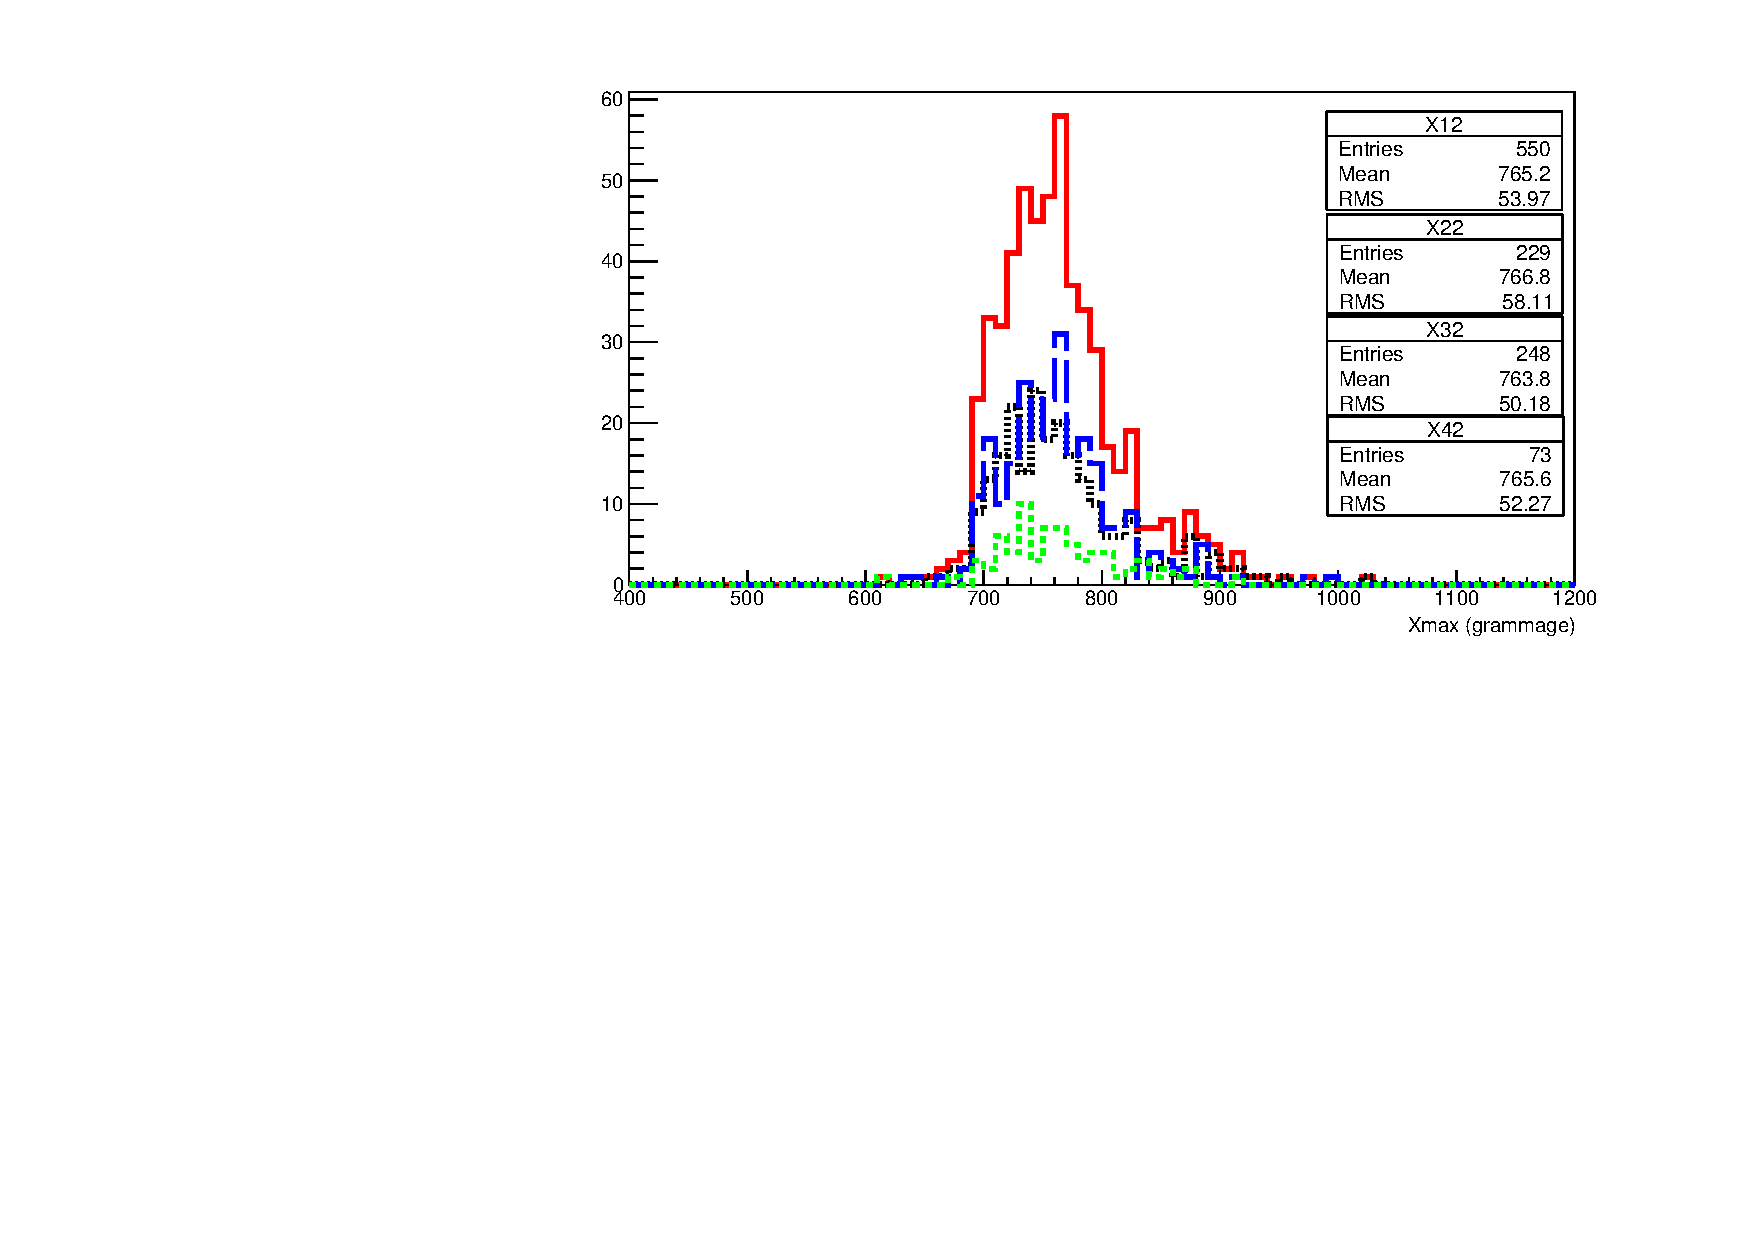
\includegraphics[width=\textwidth]{/home/tsudholz/PhD/Thesis/chapters/graphs/CloudFlags/NormHist_Xmax_FailedCloudCut_logE_18_75to19_0_Comb.pdf}
\caption{Distribution of the energy of events within the bin of log(E) of 18.75 to 19.0. Red (X12) denotes all event that failed the cloud cuts, black (X22) denotes events that failed the cloud camera/lidar cut, blue (X32) denotes events that failed the GOES data cut and green (X42) are events that have fail a combination of CLF/XLF, GOES and Cloud camera cut.} \label{fig:CloudFlag_XmaxFailed_18.75}
\end{figure}

\begin{figure}[!p]
\centering
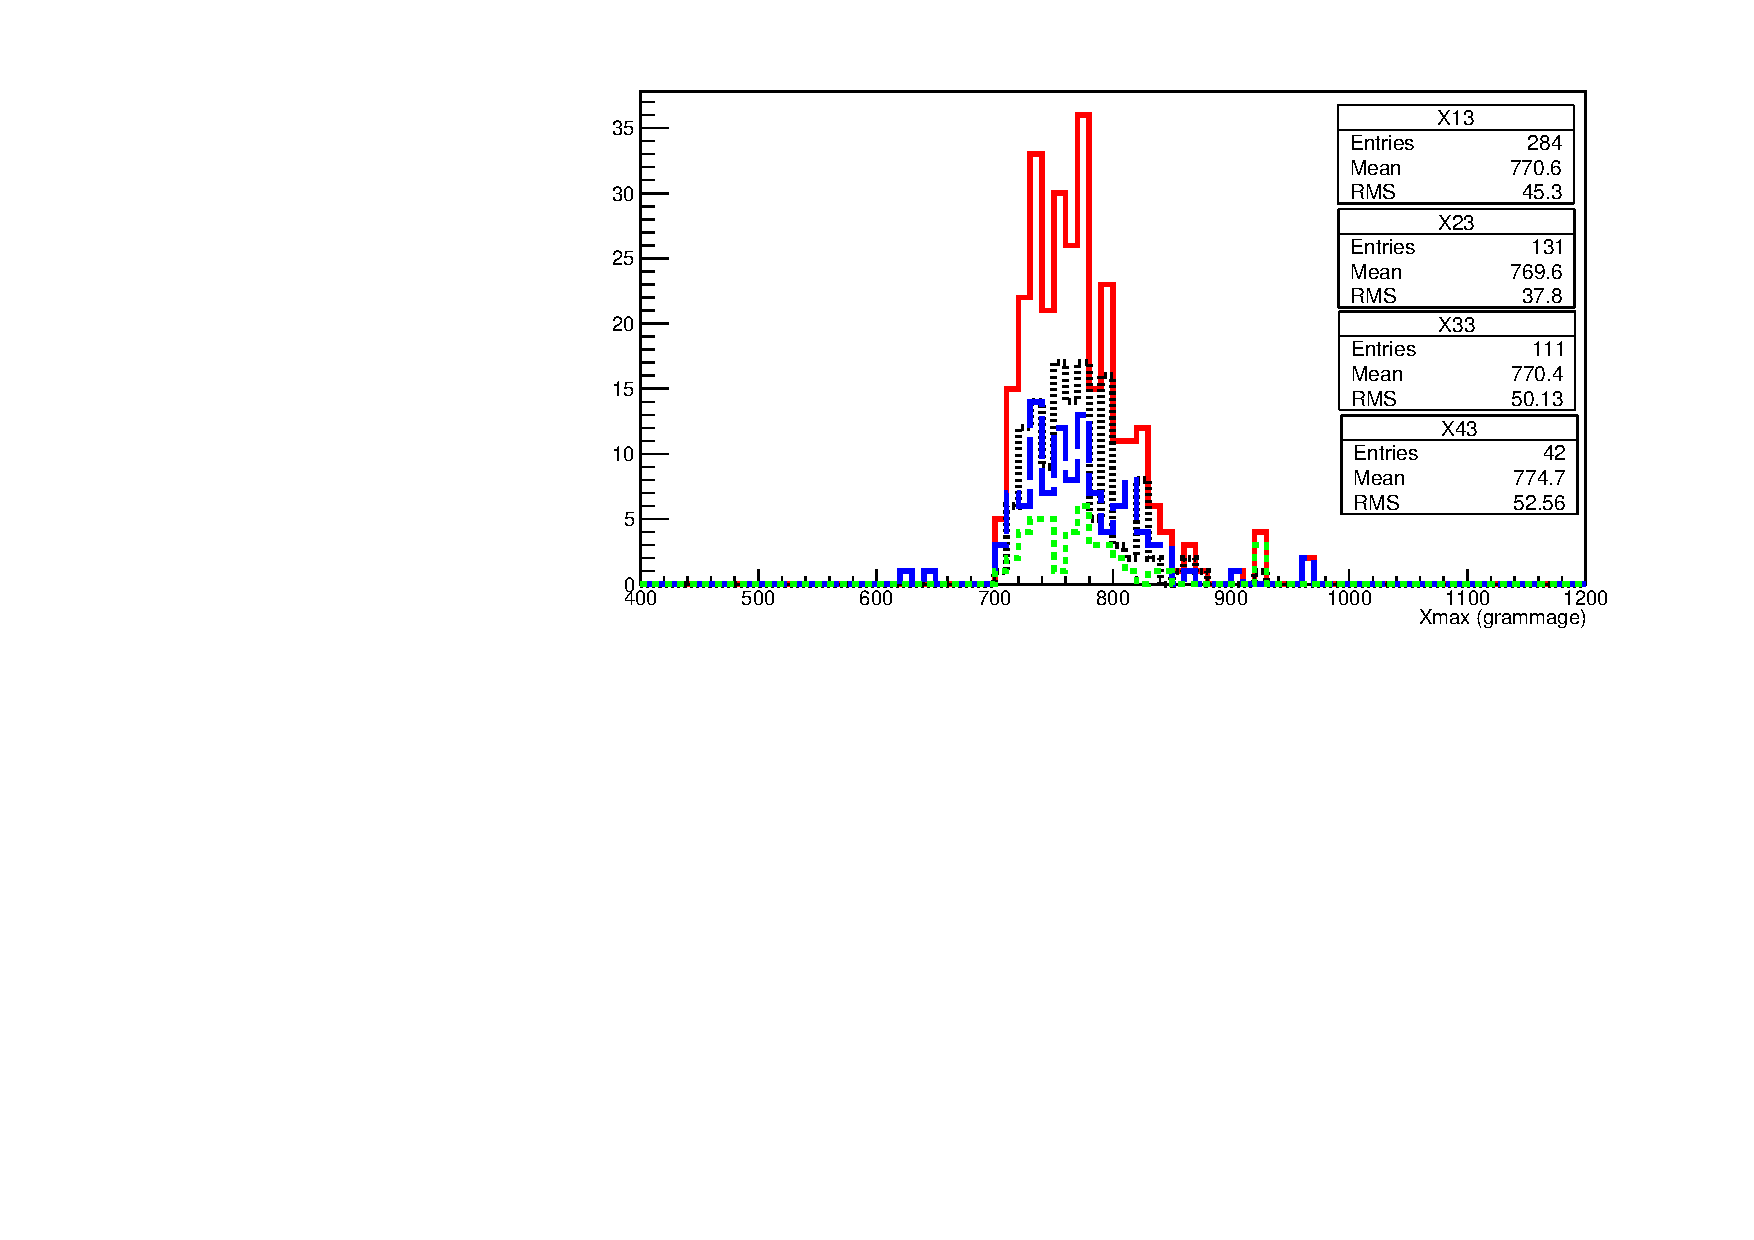
\includegraphics[width=\textwidth]{/home/tsudholz/PhD/Thesis/chapters/graphs/CloudFlags/NormHist_Xmax_FailedCloudCut_logE_19_0to19_25_Comb.pdf}
\caption{Distribution of the energy of events within the bin of log(E) of 19.0 to 19.25. Red (X13) denotes all event that failed the cloud cuts, black (X23) denotes events that failed the cloud camera/lidar cut, blue (X33) denotes events that failed the GOES data cut and green (X43) are events that have fail a combination of CLF/XLF, GOES and Cloud camera cut.} \label{fig:CloudFlag_XmaxFailed_19.0}
\end{figure}

\begin{figure}[!p]
\centering
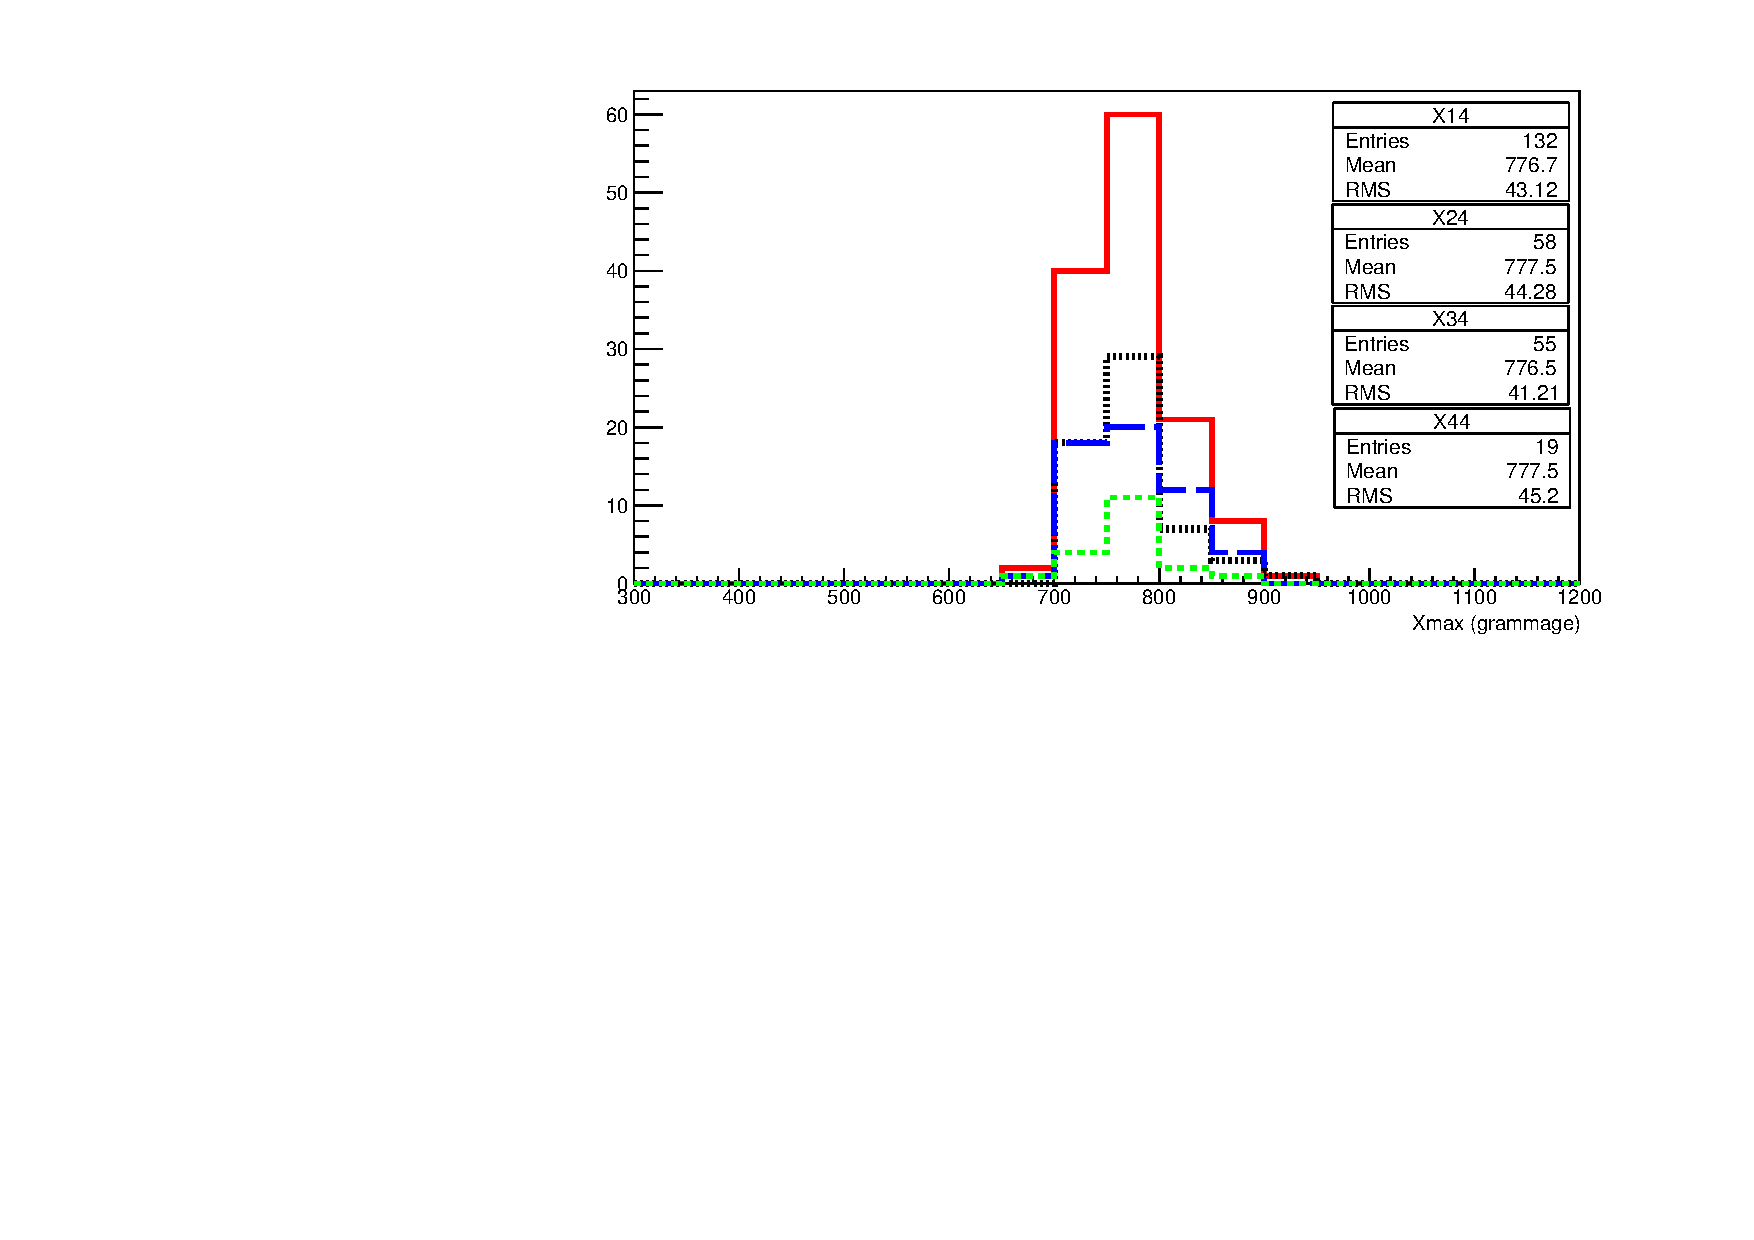
\includegraphics[width=\textwidth]{/home/tsudholz/PhD/Thesis/chapters/graphs/CloudFlags/NormHist_Xmax_FailedCloudCut_logE_19_25to19_5_Comb.pdf}
\caption{Distribution of the energy of events within the bin of log(E) of 19.25 to 19.5. Red (X14) denotes all event that failed the cloud cuts, black (X24) denotes events that failed the cloud camera/lidar cut, blue (X34) denotes events that failed the GOES data cut and green (X44) are events that have fail a combination of CLF/XLF, GOES and Cloud camera cut.} \label{fig:CloudFlag_XmaxFailed_19.25}
\end{figure}

\begin{figure}[!p]
\centering
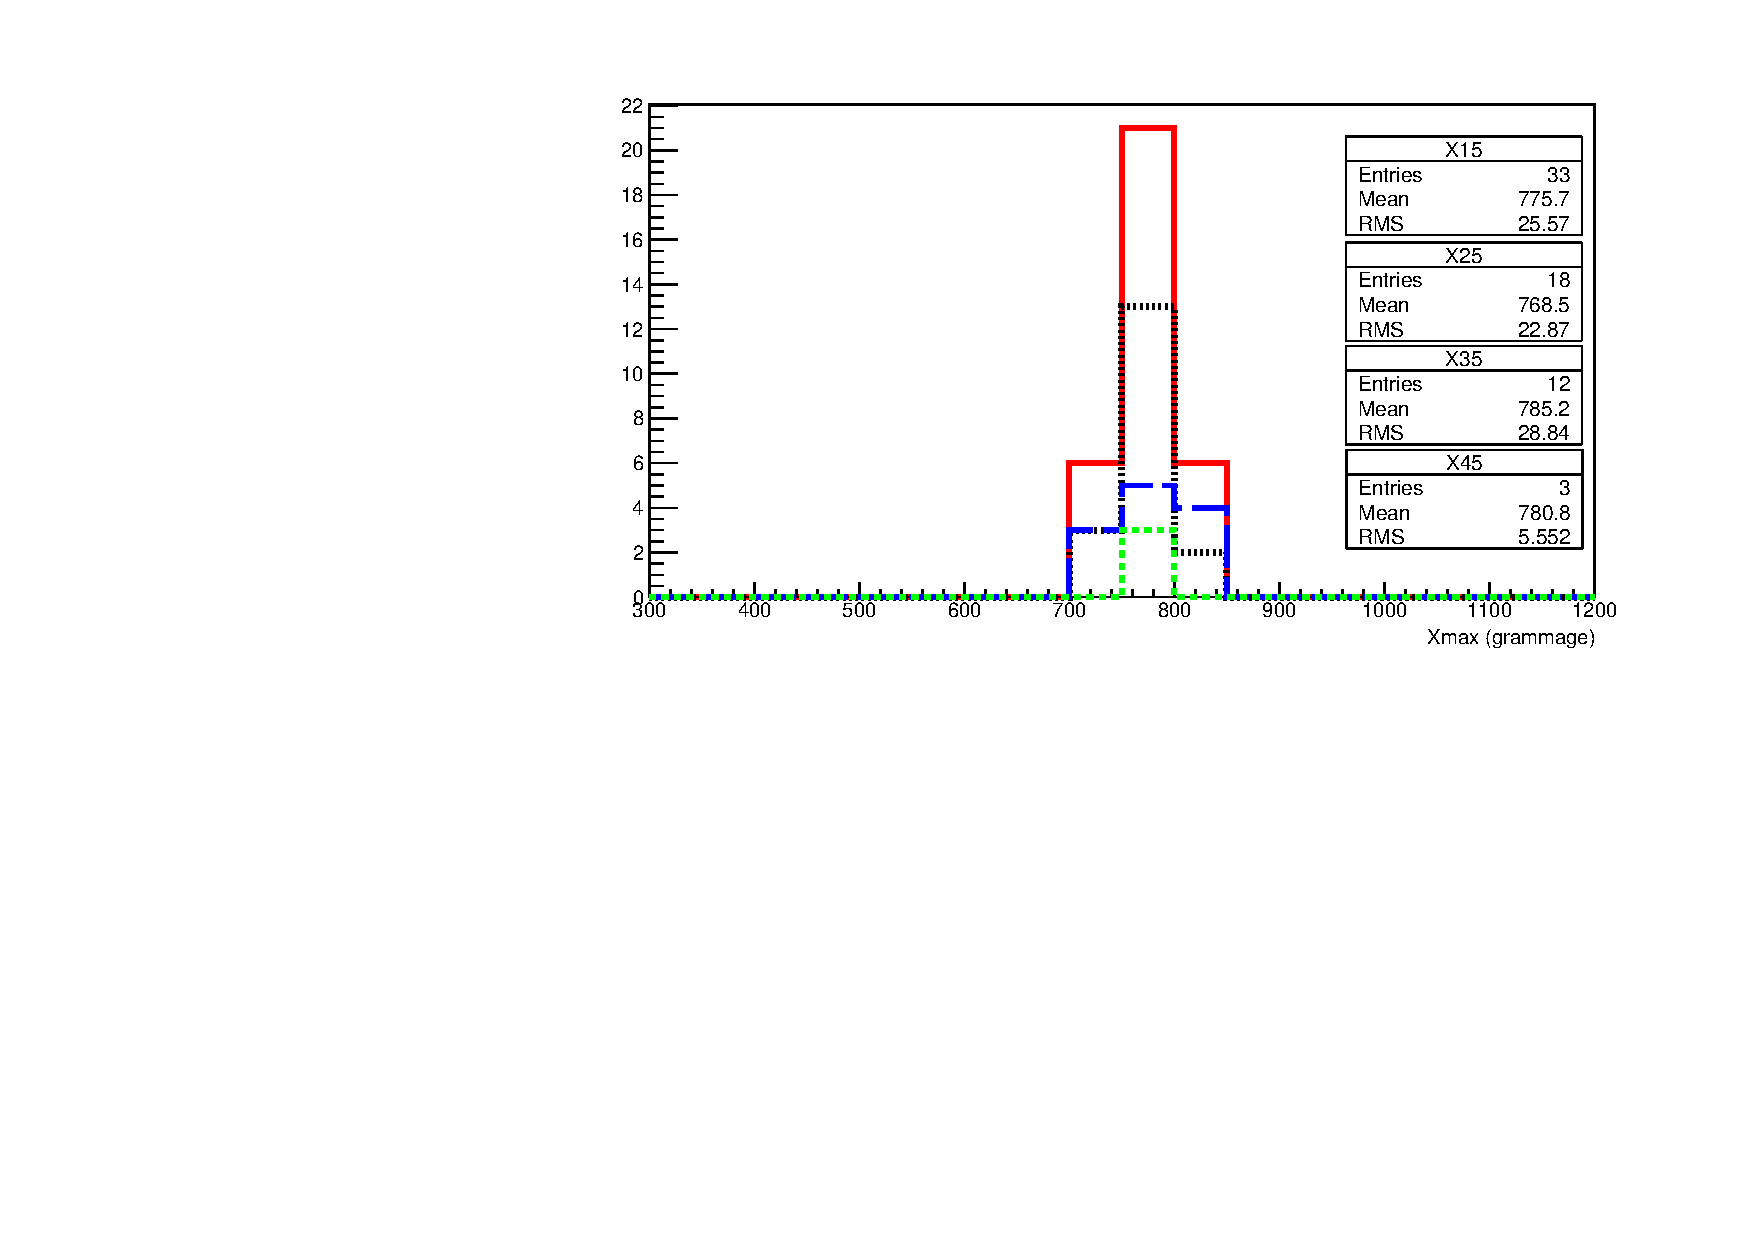
\includegraphics[width=\textwidth]{/home/tsudholz/PhD/Thesis/chapters/graphs/CloudFlags/NormHist_Xmax_FailedCloudCut_logE_Greater19_5_Comb.pdf}
\caption{Distribution of the energy of events within the bin of log(E) of greater than 19.5. Red (X15) denotes all event that failed the cloud cuts, black (X25) denotes events that failed the cloud camera/lidar cut, blue (X35) denotes events that failed the GOES data cut and green (X45) are events that have fail a combination of CLF/XLF, GOES and Cloud camera cut.} \label{fig:CloudFlag_XmaxFailed_19.5}
\end{figure}

Figures \ref{fig:CloudFlag_XmaxFailed_18.0} to Figure \ref{fig:CloudFlag_XmaxFailed_19.5} show the distributions of events that failed the cloud cuts split into 3 different flag types. Red denotes all event that failed the cloud cuts, black denotes events that failed the cloud camera/lidar cut, blue denotes events that failed the GOES data cut and green are events that have fail a combination of CLF/XLF, GOES and Cloud camera cut. 

These distributions show that the majority of events are rejected by the cloud camera/lidar cut or by the GOES satellite cut. A smaller faction of events are rejected by a combination of CLF/XLF, GOES and Cloud camera/lidar cut.

\subsection{Graphical Examples of Events from within the tails of the Xmax distributions}

% Events that would fail the cloud cut only

\begin{figure}[!p]
\centering
  \settoheight{\tempheight}{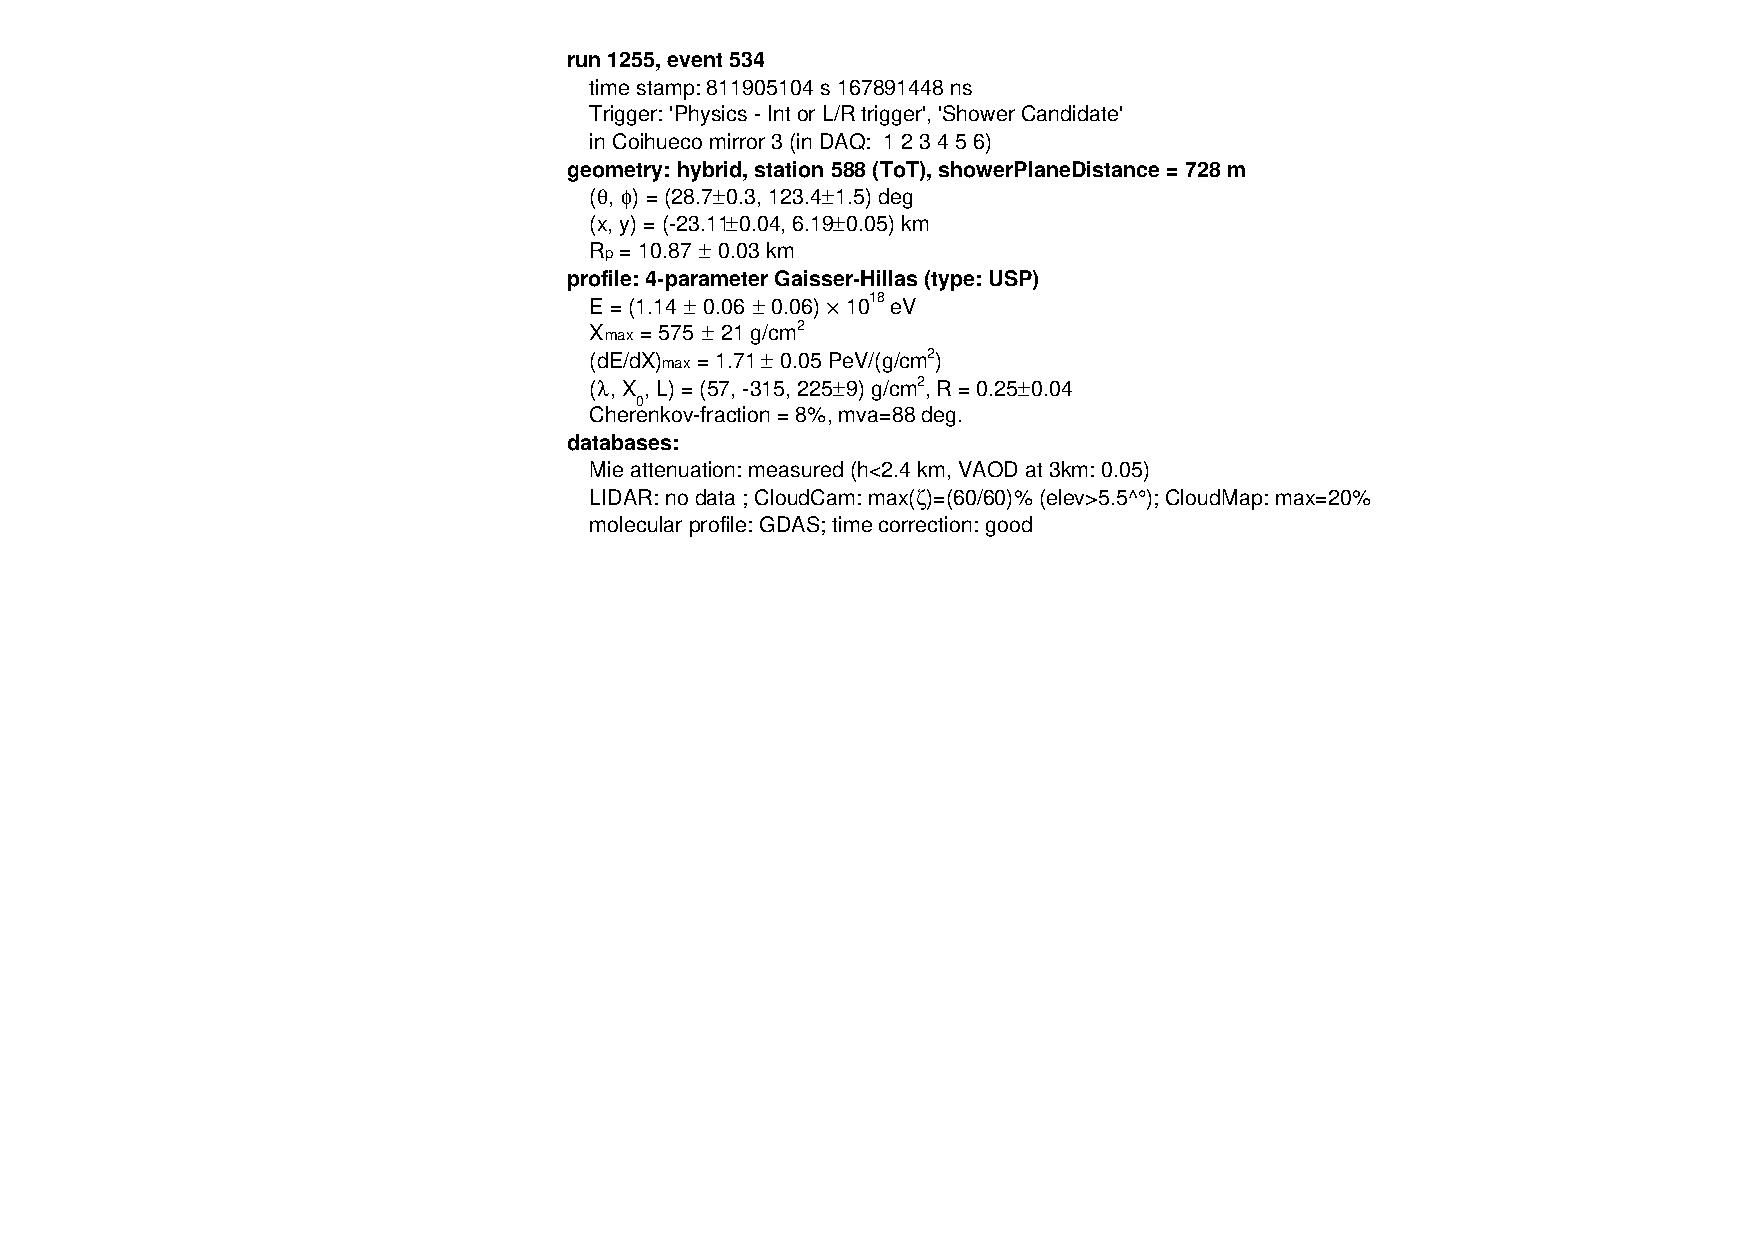
\includegraphics[width=0.45\textwidth , trim = 0 0 5.5cm 0]{/home/tsudholz/PhD/Thesis/chapters/graphs/CloudFlags/CloudCut_Events_Failed/Auger_52704749200_FdEventInfo.pdf}}
 \vspace{2cm}
  \begin{subfigure}[b]{\textwidth}
  \centering
  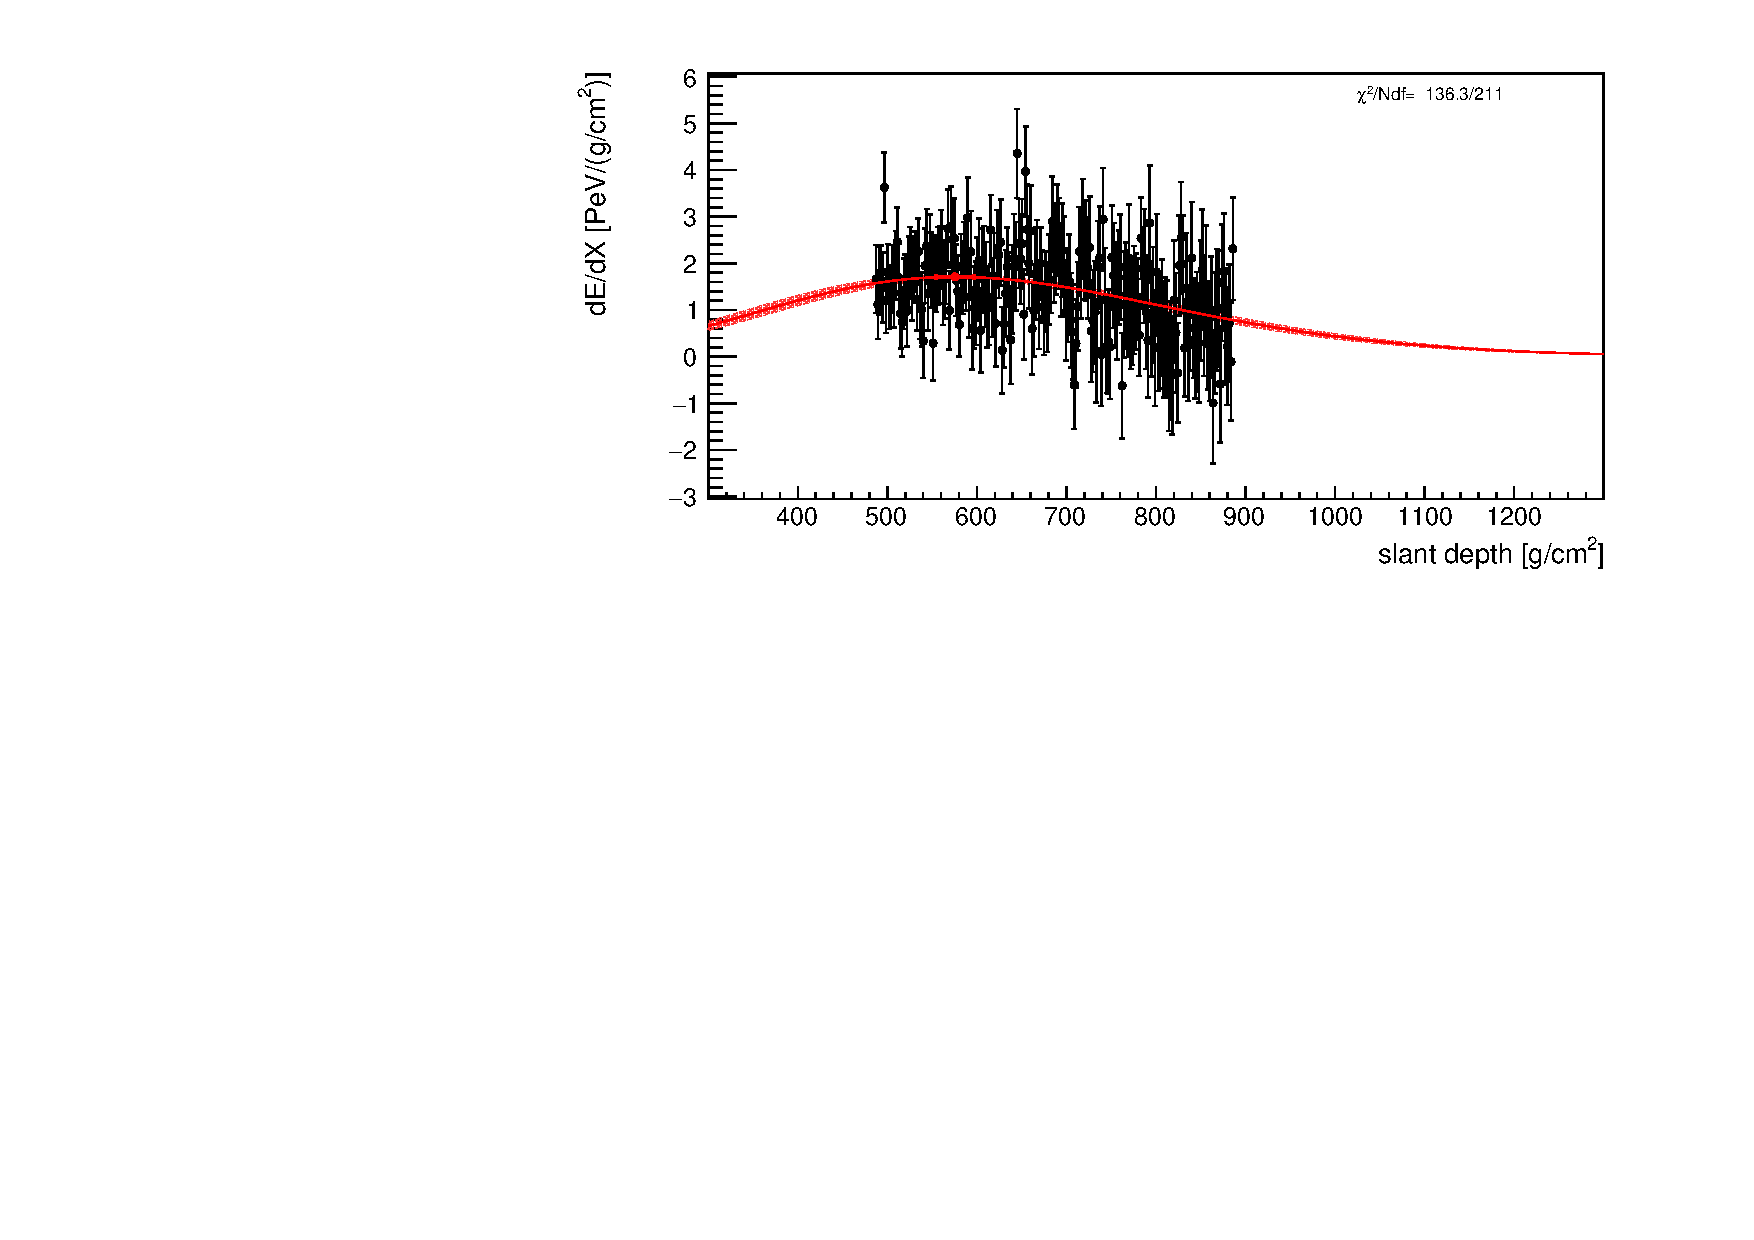
\includegraphics[width=\textwidth]{/home/tsudholz/PhD/Thesis/chapters/graphs/CloudFlags/CloudCut_Events_Failed/Auger_52704749200_SlantDepth.pdf}
  \caption{FD profile of the energy deposited as a function of atmospheric depth.}
  \end{subfigure}
 \vspace{0.5cm}
  \begin{subfigure}[b]{0.45\textwidth}
  	\centering
  	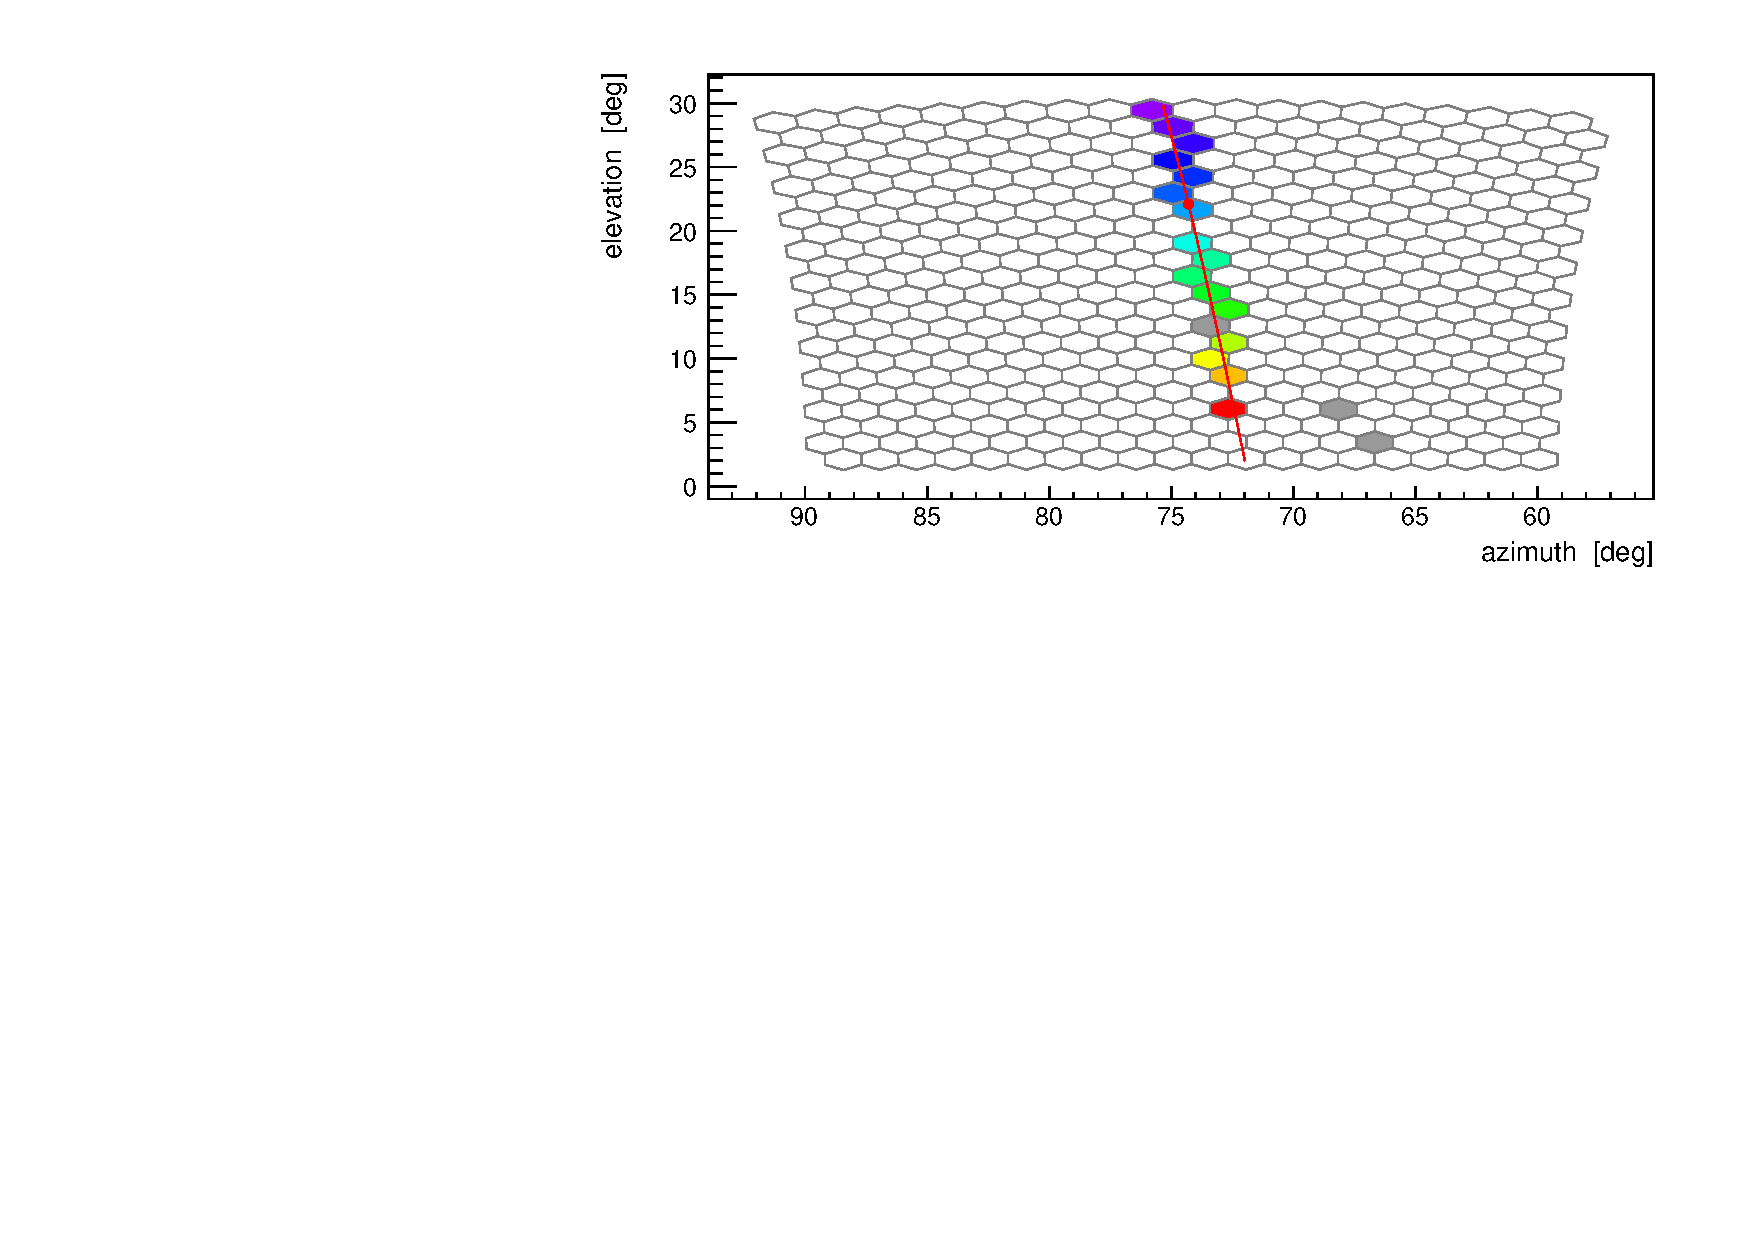
\includegraphics[width=\textwidth , height=\tempheight]{/home/tsudholz/PhD/Thesis/chapters/graphs/CloudFlags/CloudCut_Events_Failed/Auger_52704749200_FdProfile.pdf}
  	\caption{FD light profile}
  \end{subfigure}
  \begin{subfigure}[b]{0.45\textwidth}
  	\centering
  	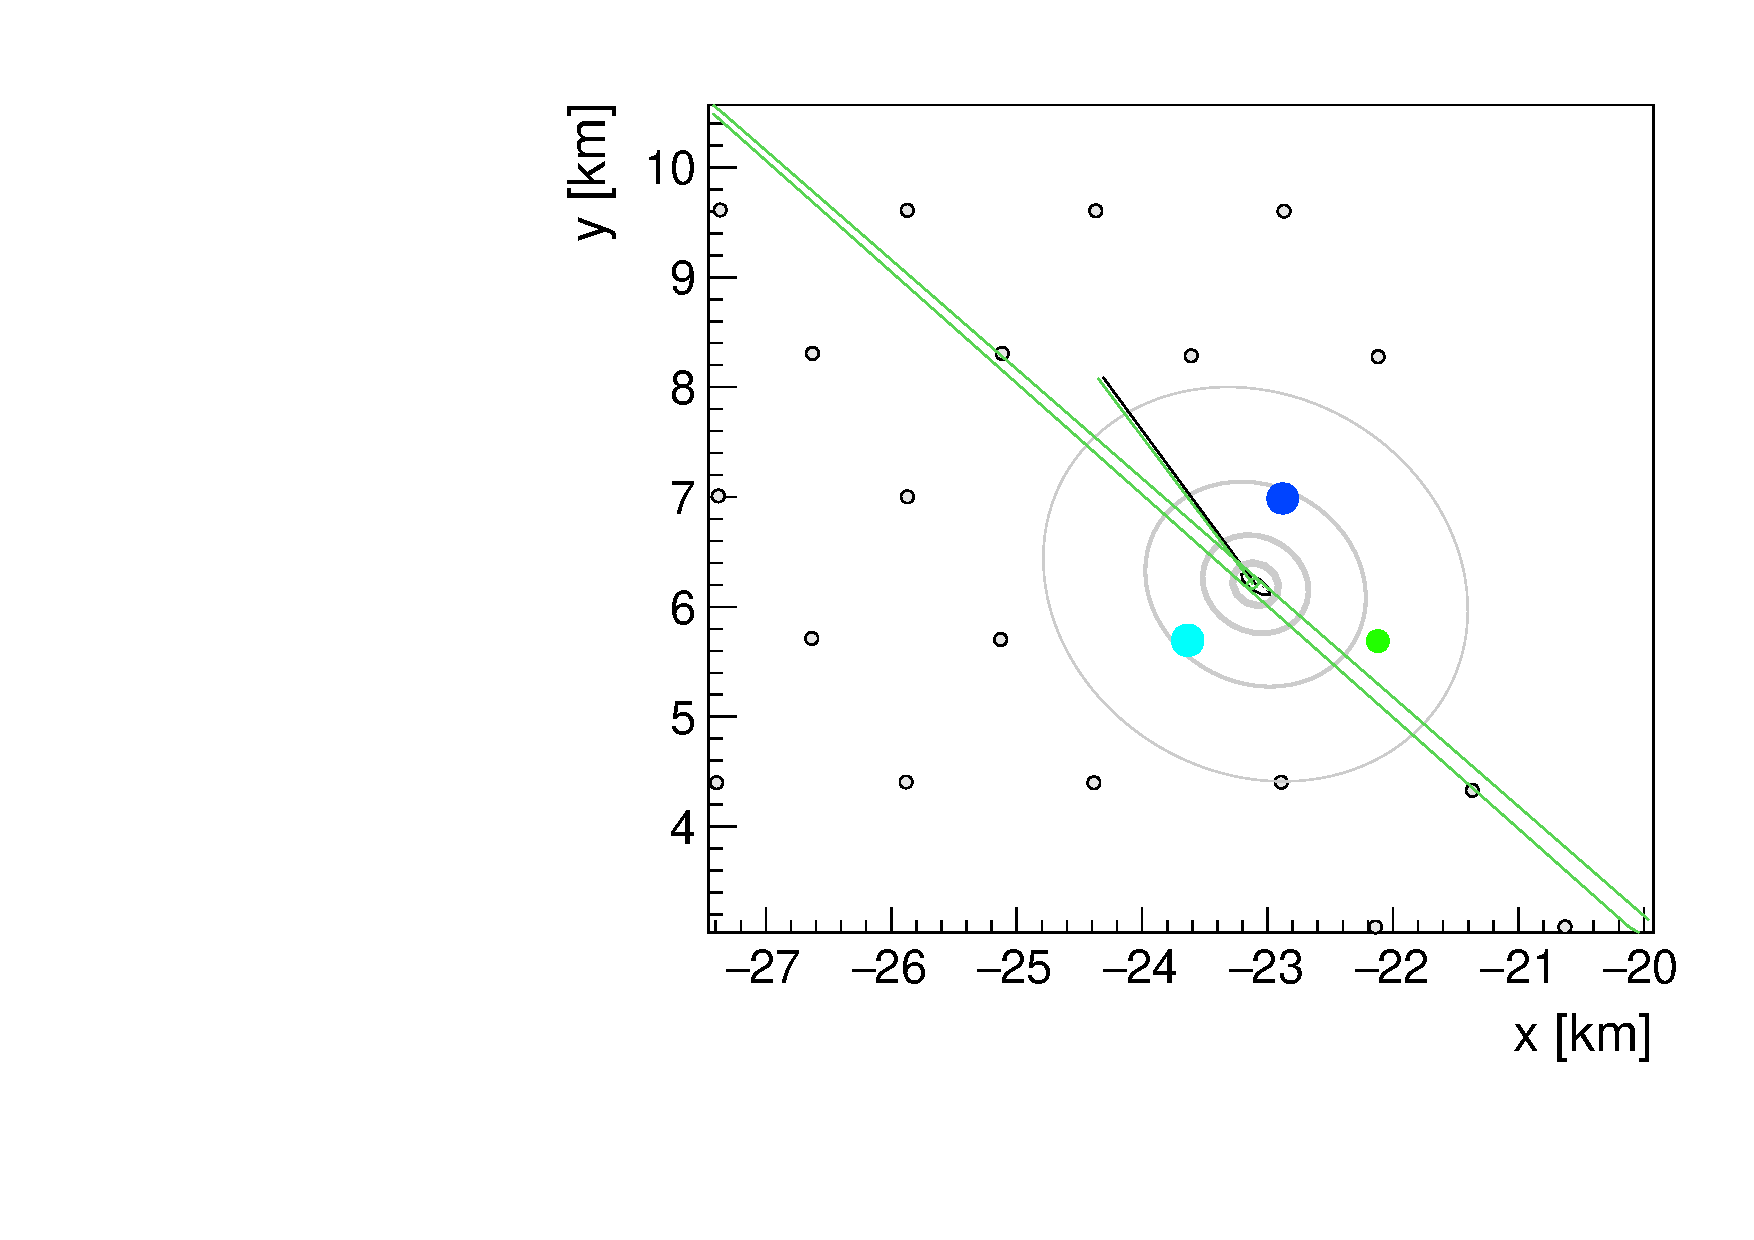
\includegraphics[width=0.8\textwidth , height=\tempheight]{/home/tsudholz/PhD/Thesis/chapters/graphs/CloudFlags/CloudCut_Events_Failed/Auger_52704749200_SdProfile.pdf}
  	\caption{SD tank triggered profile}
  \end{subfigure}

  \begin{subfigure}[b]{0.45\textwidth}
  	\centering
	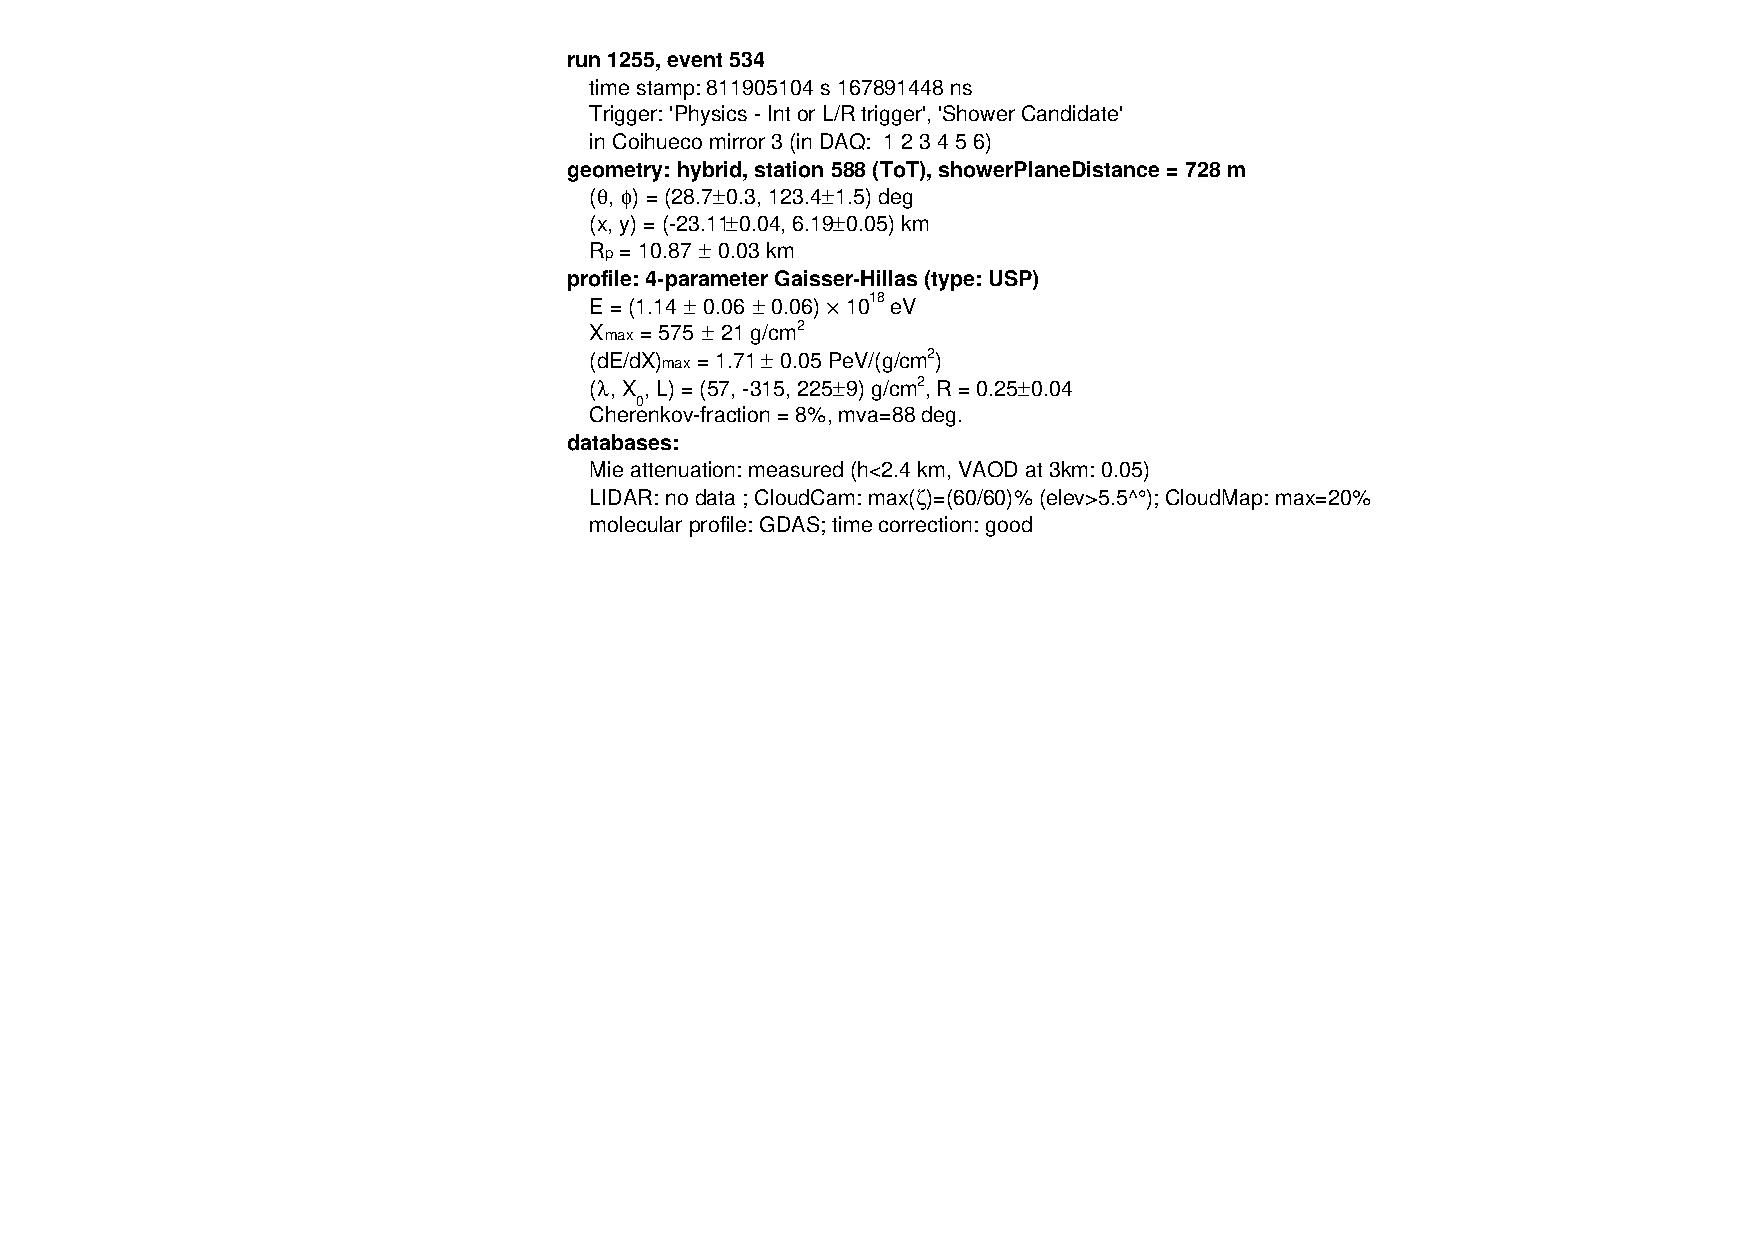
\includegraphics[height=\tempheight , trim = 0 0 5.5cm 0]{/home/tsudholz/PhD/Thesis/chapters/graphs/CloudFlags/CloudCut_Events_Failed/Auger_52704749200_FdEventInfo.pdf}
  	\caption{FD Event Info}
  \end{subfigure}
  \begin{subfigure}[b]{0.45\textwidth}
  	\centering
	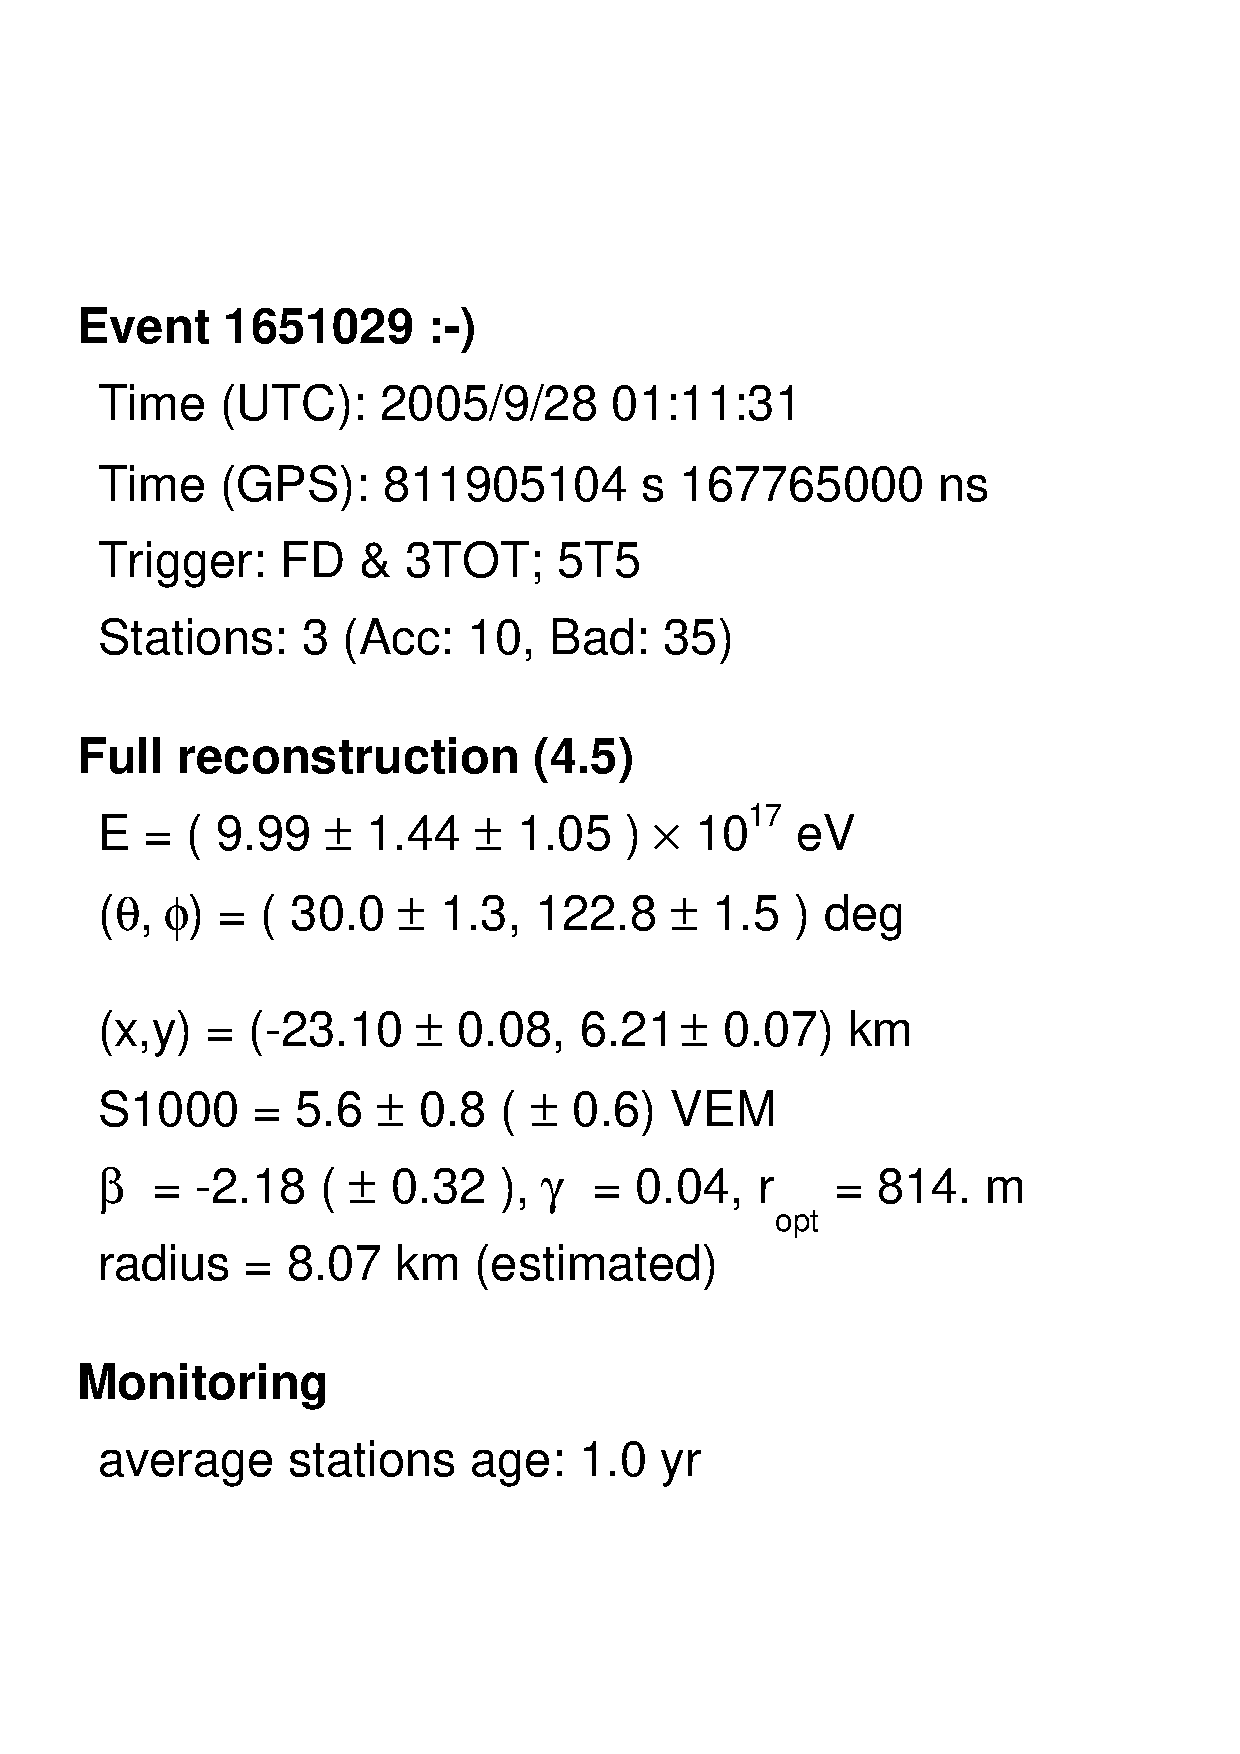
\includegraphics[height=\tempheight]{/home/tsudholz/PhD/Thesis/chapters/graphs/CloudFlags/CloudCut_Events_Failed/Auger_52704749200_SdEventInfo.pdf}
  	\caption{SD Event Info}
  \end{subfigure}
  \caption{Example of an Auger event that would fail the cloud selection cut from EventBrowser}
\end{figure}

\begin{figure}[!p]
\centering
  \settoheight{\tempheight}{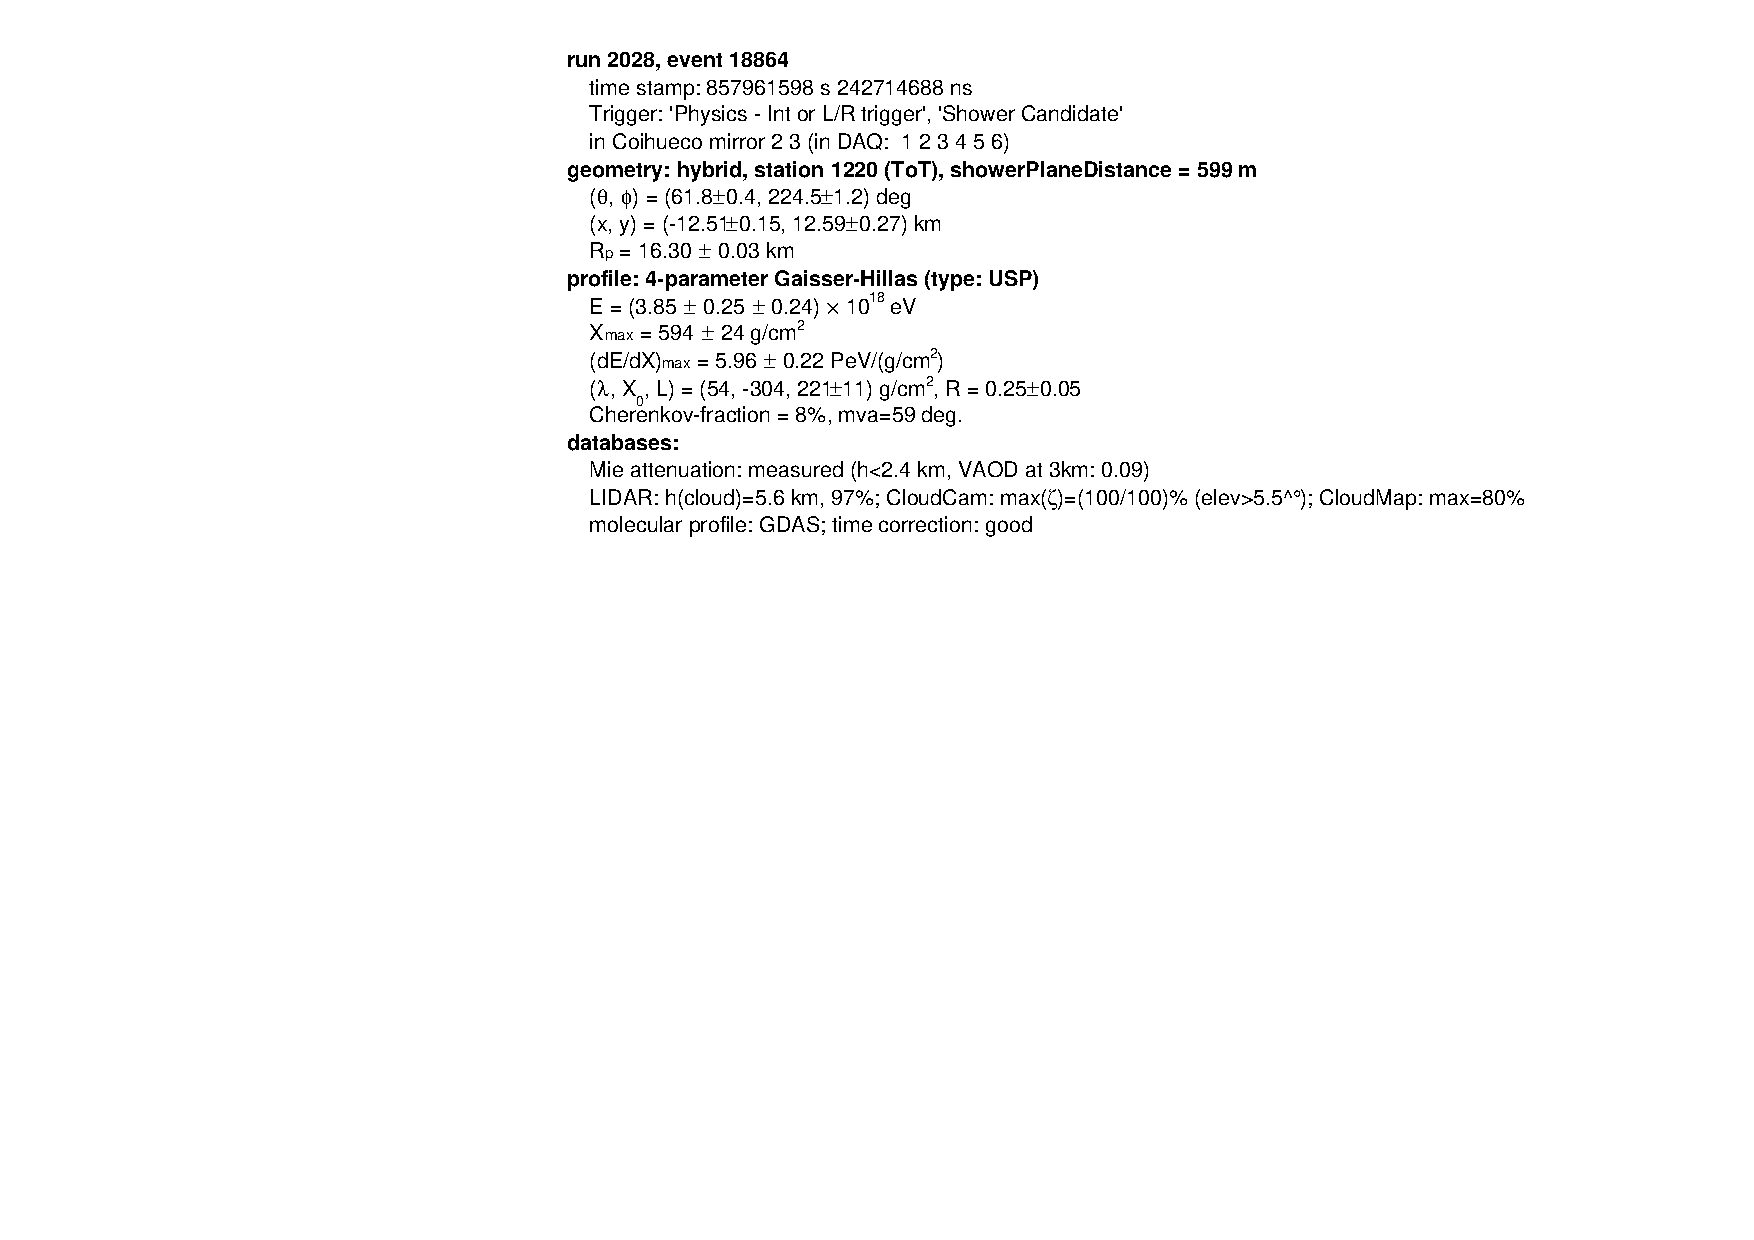
\includegraphics[width=0.45\textwidth , trim = 0 0 5.5cm 0]{/home/tsudholz/PhD/Thesis/chapters/graphs/CloudFlags/CloudCut_Events_Failed/Auger_70735278500_FdEventInfo.pdf}}
 \vspace{2cm}
  \begin{subfigure}[b]{\textwidth}
  \centering
  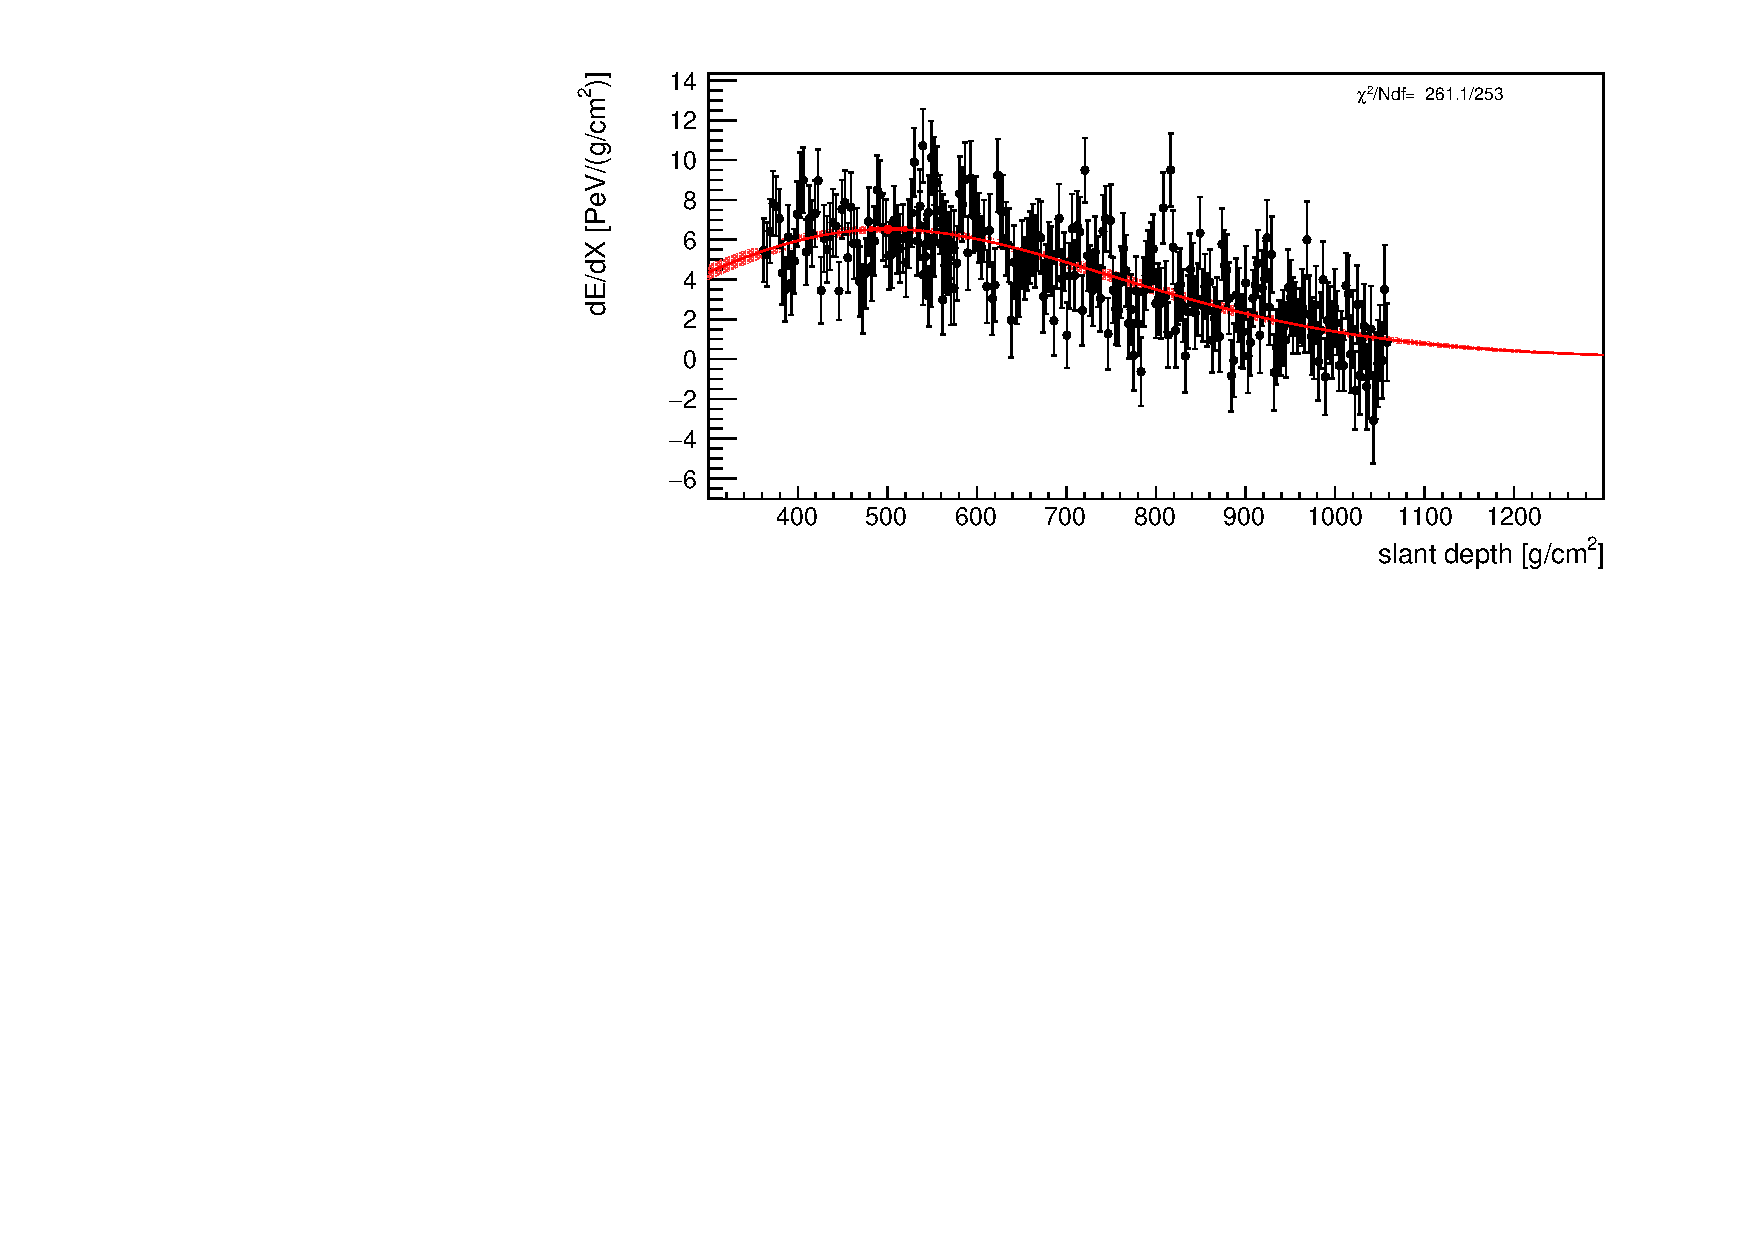
\includegraphics[width=\textwidth]{/home/tsudholz/PhD/Thesis/chapters/graphs/CloudFlags/CloudCut_Events_Failed/Auger_160416430001_SlantDepth.pdf}
  \caption{FD profile of the energy deposited as a function of atmospheric depth.}
  \end{subfigure}
 \vspace{0.5cm}
  \begin{subfigure}[b]{0.45\textwidth}
  	\centering
  	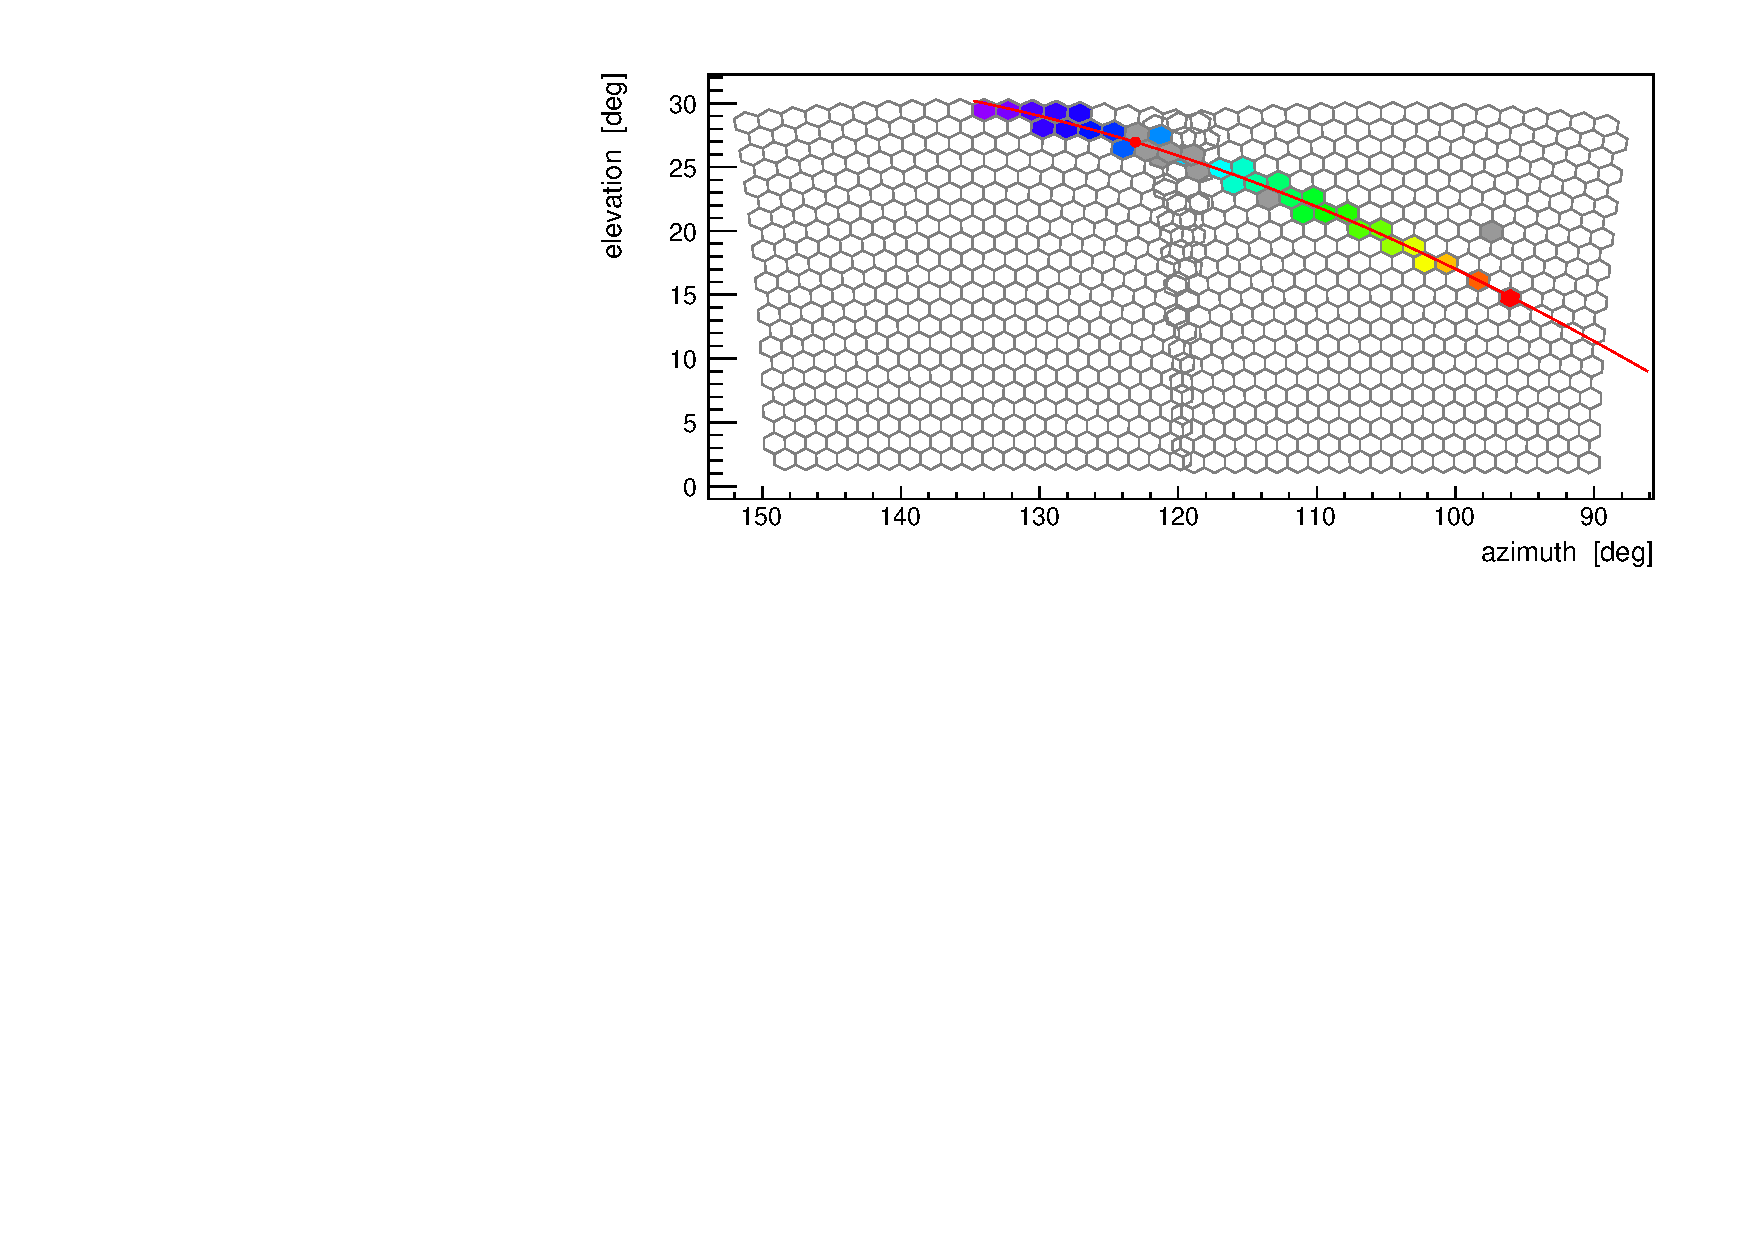
\includegraphics[width=\textwidth , height=\tempheight]{/home/tsudholz/PhD/Thesis/chapters/graphs/CloudFlags/CloudCut_Events_Failed/Auger_160416430001_FdProfile.pdf}
  	\caption{FD light profile}
  \end{subfigure}
  \begin{subfigure}[b]{0.45\textwidth}
  	\centering
  	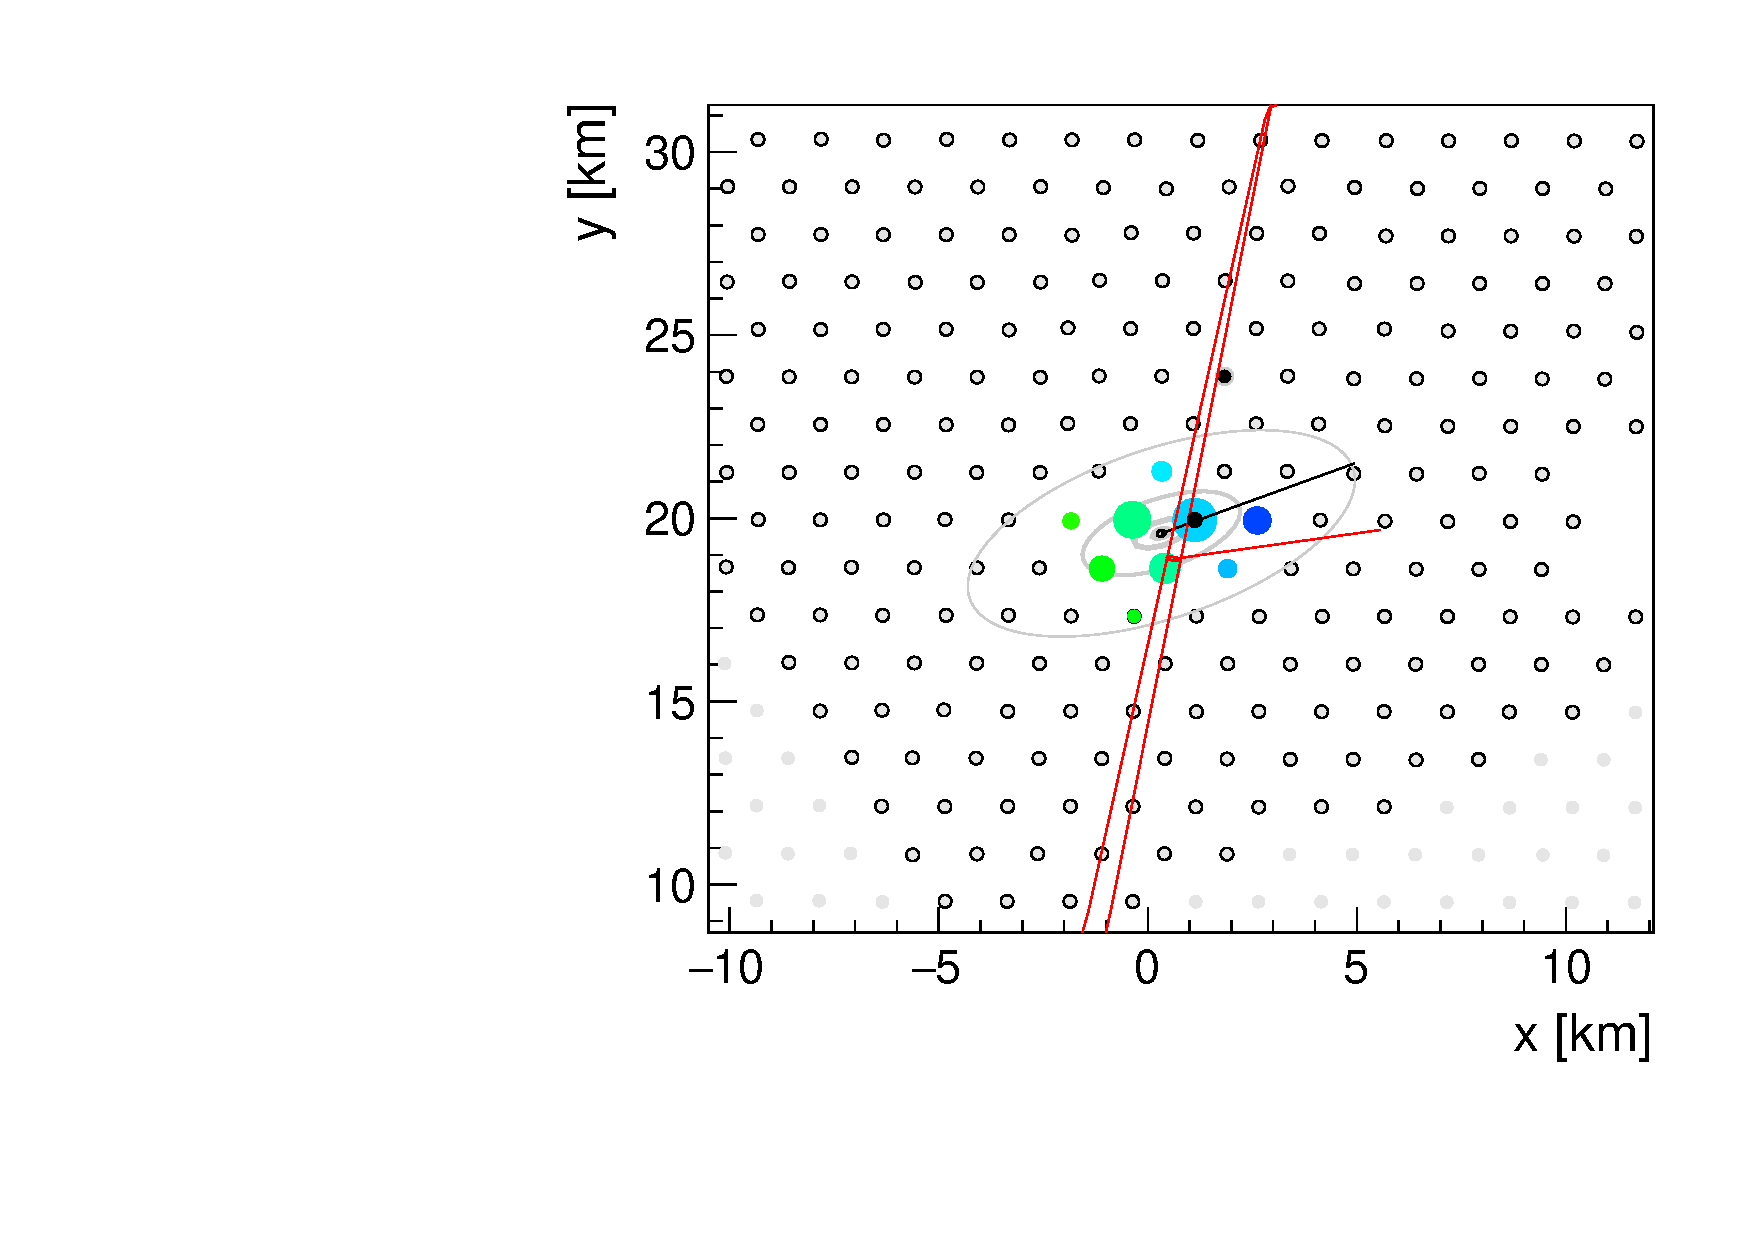
\includegraphics[width=0.8\textwidth , height=\tempheight]{/home/tsudholz/PhD/Thesis/chapters/graphs/CloudFlags/CloudCut_Events_Failed/Auger_160416430001_SdProfile.pdf}
  	\caption{SD tank triggered profile}
  \end{subfigure}

  \begin{subfigure}[b]{0.45\textwidth}
  	\centering
	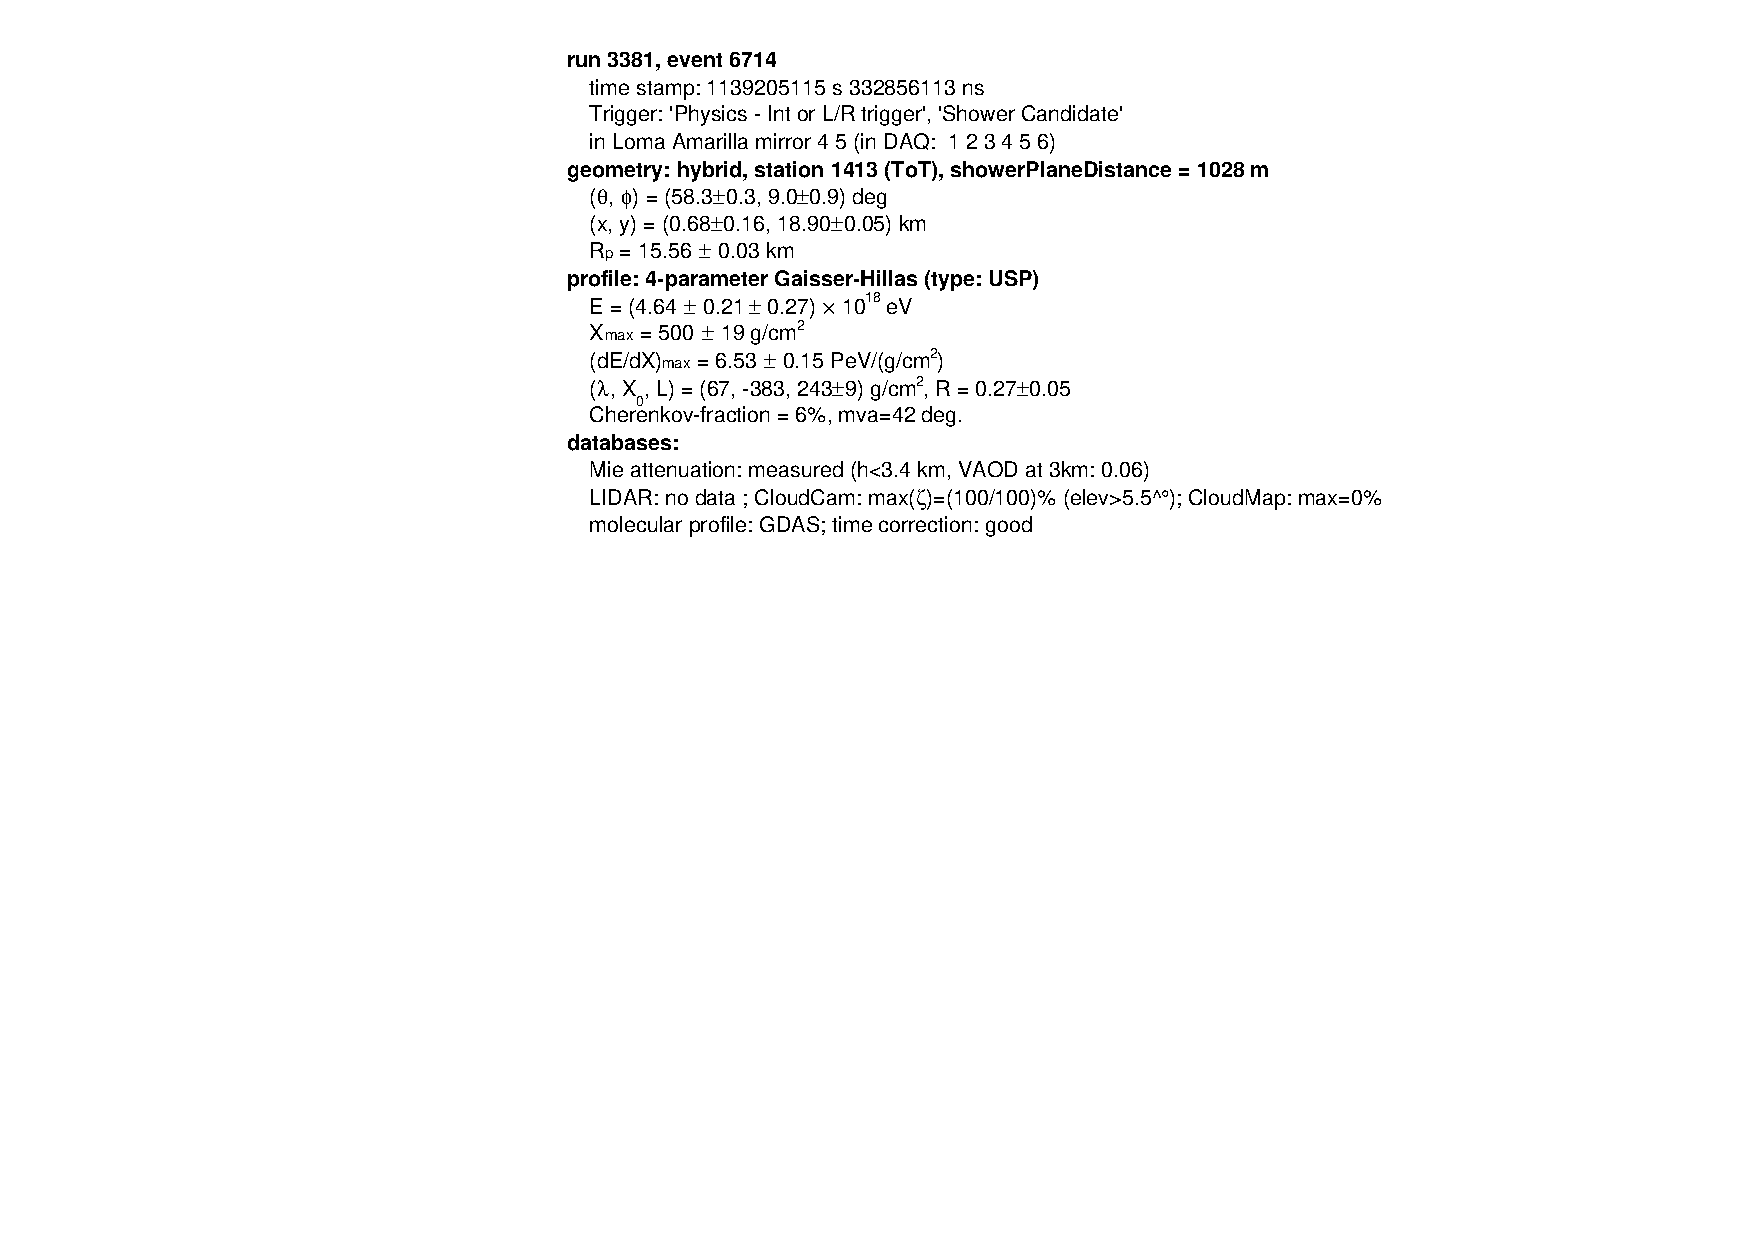
\includegraphics[height=\tempheight , trim = 0 0 5.5cm 0]{/home/tsudholz/PhD/Thesis/chapters/graphs/CloudFlags/CloudCut_Events_Failed/Auger_160416430001_FdEventInfo.pdf}
  	\caption{FD light profile}
  \end{subfigure}
  \begin{subfigure}[b]{0.45\textwidth}
  	\centering
	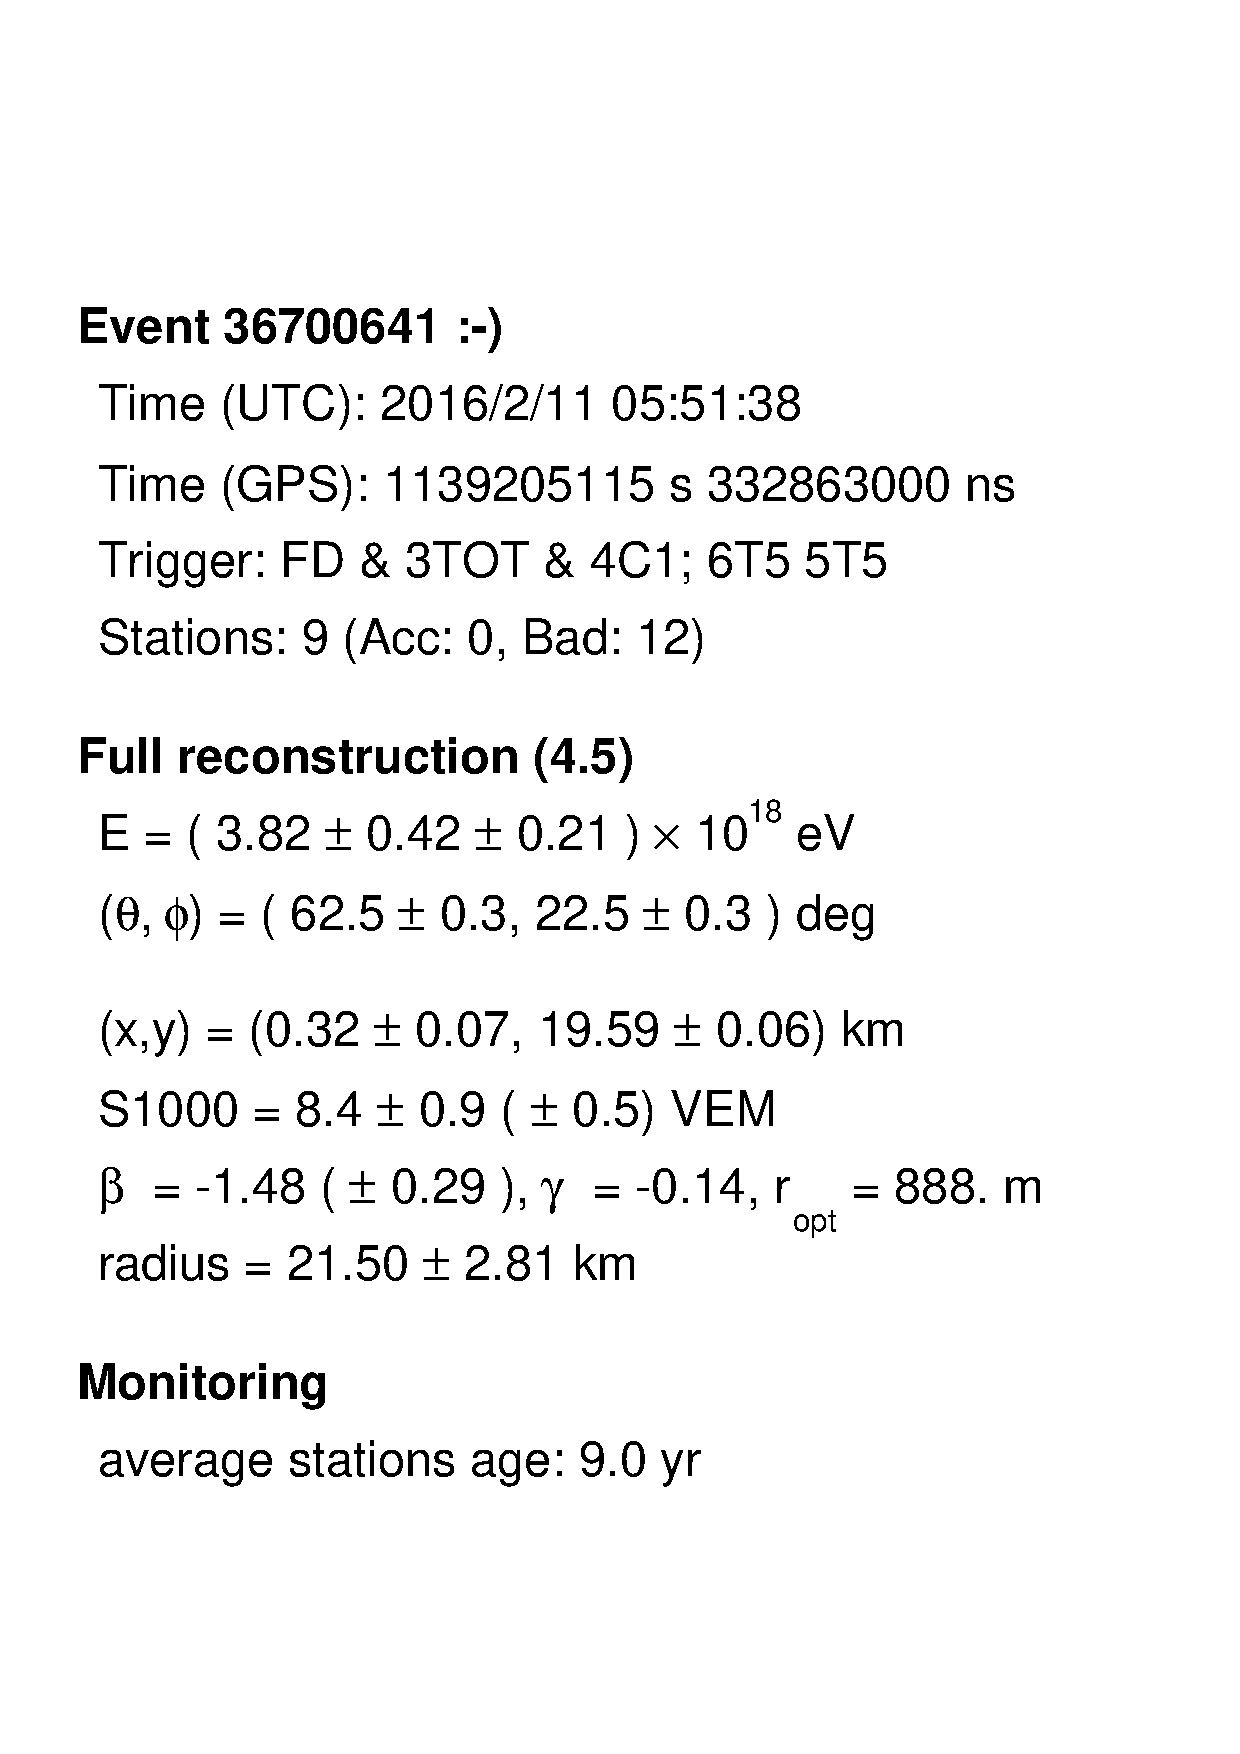
\includegraphics[height=\tempheight]{/home/tsudholz/PhD/Thesis/chapters/graphs/CloudFlags/CloudCut_Events_Failed/Auger_160416430001_SdEventInfo.pdf}
  	\caption{SD tank triggered profile}
  \end{subfigure}
  \caption{Example of an Auger event that would fail the cloud selection cut from EventBrowser}
\end{figure}

\begin{figure}[!p]
\centering
  \settoheight{\tempheight}{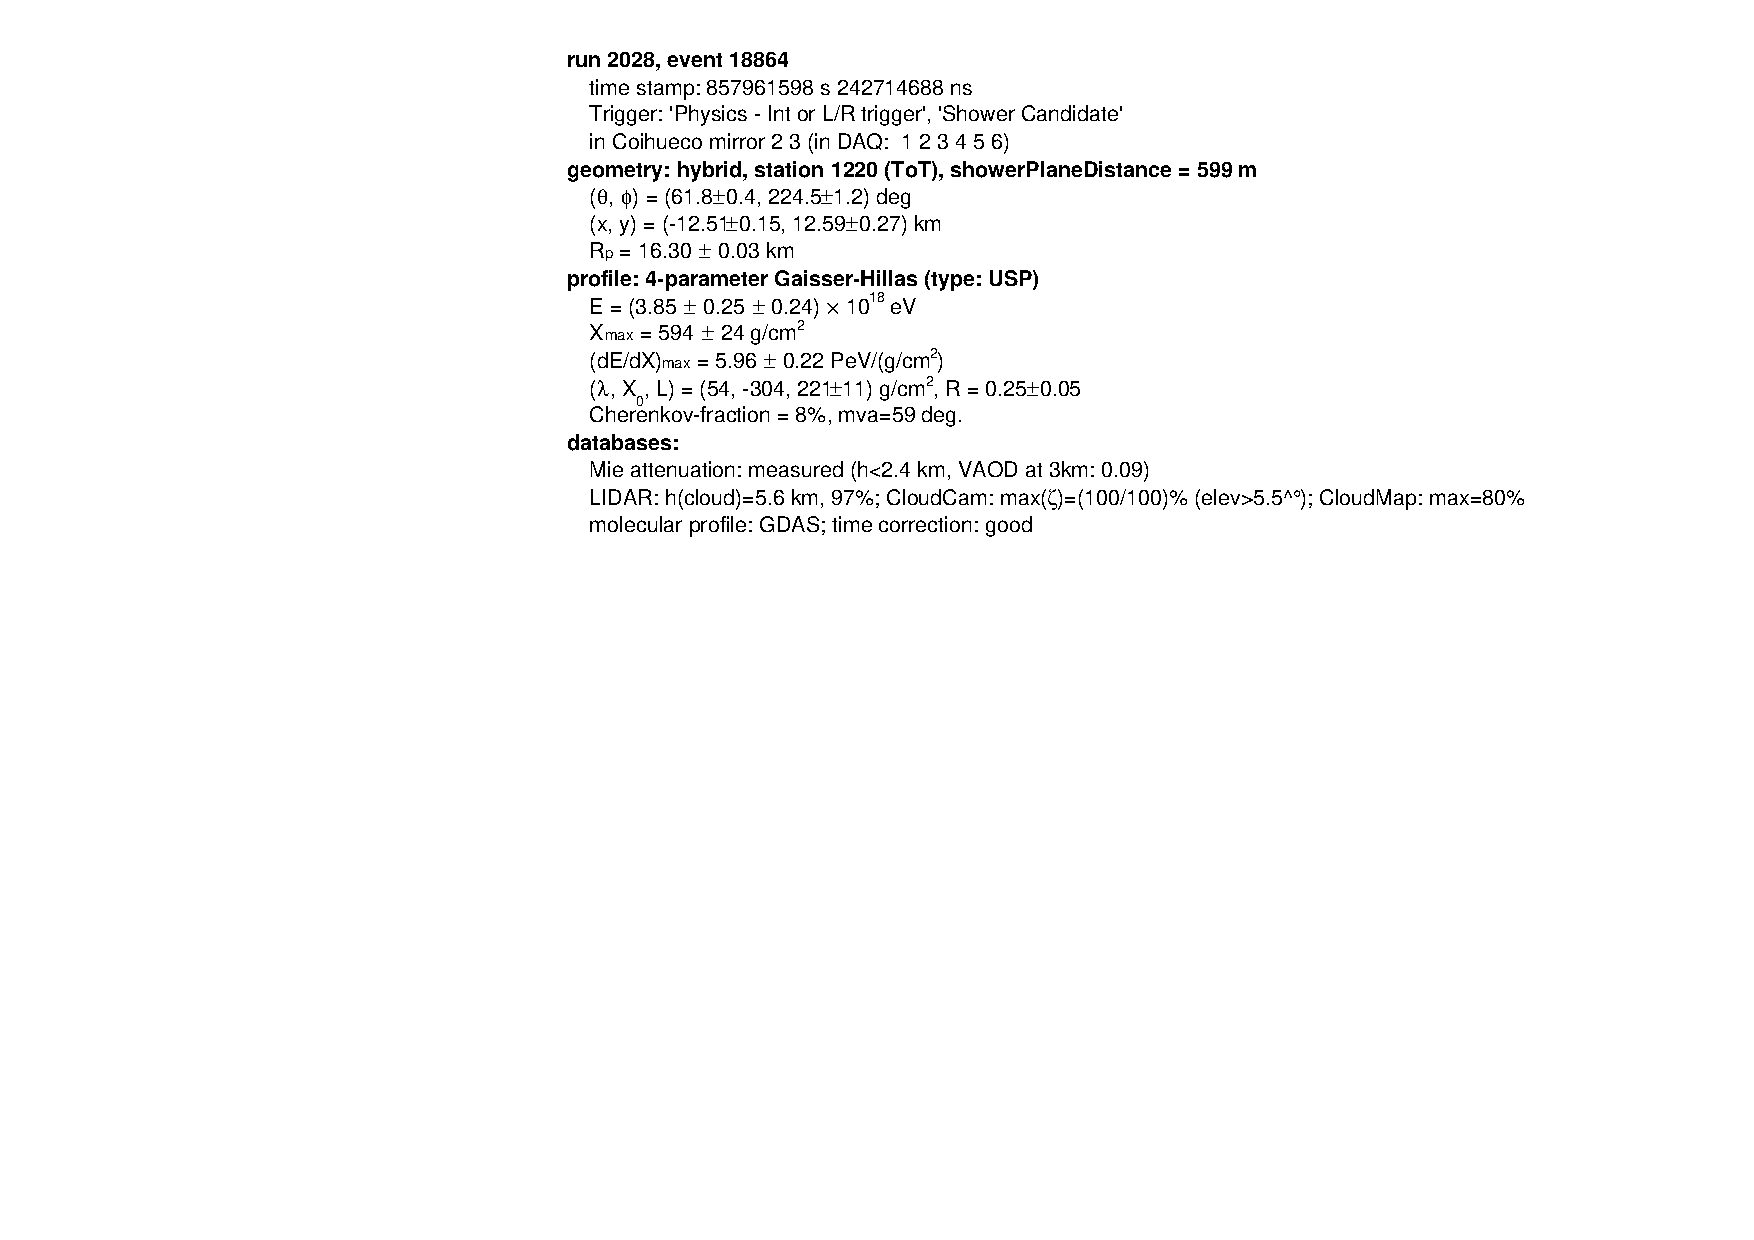
\includegraphics[width=0.45\textwidth , trim = 0 0 5.5cm 0]{/home/tsudholz/PhD/Thesis/chapters/graphs/CloudFlags/CloudCut_Events_Failed/Auger_70735278500_FdEventInfo.pdf}}
 \vspace{2cm}
  \begin{subfigure}[b]{\textwidth}
  \centering
  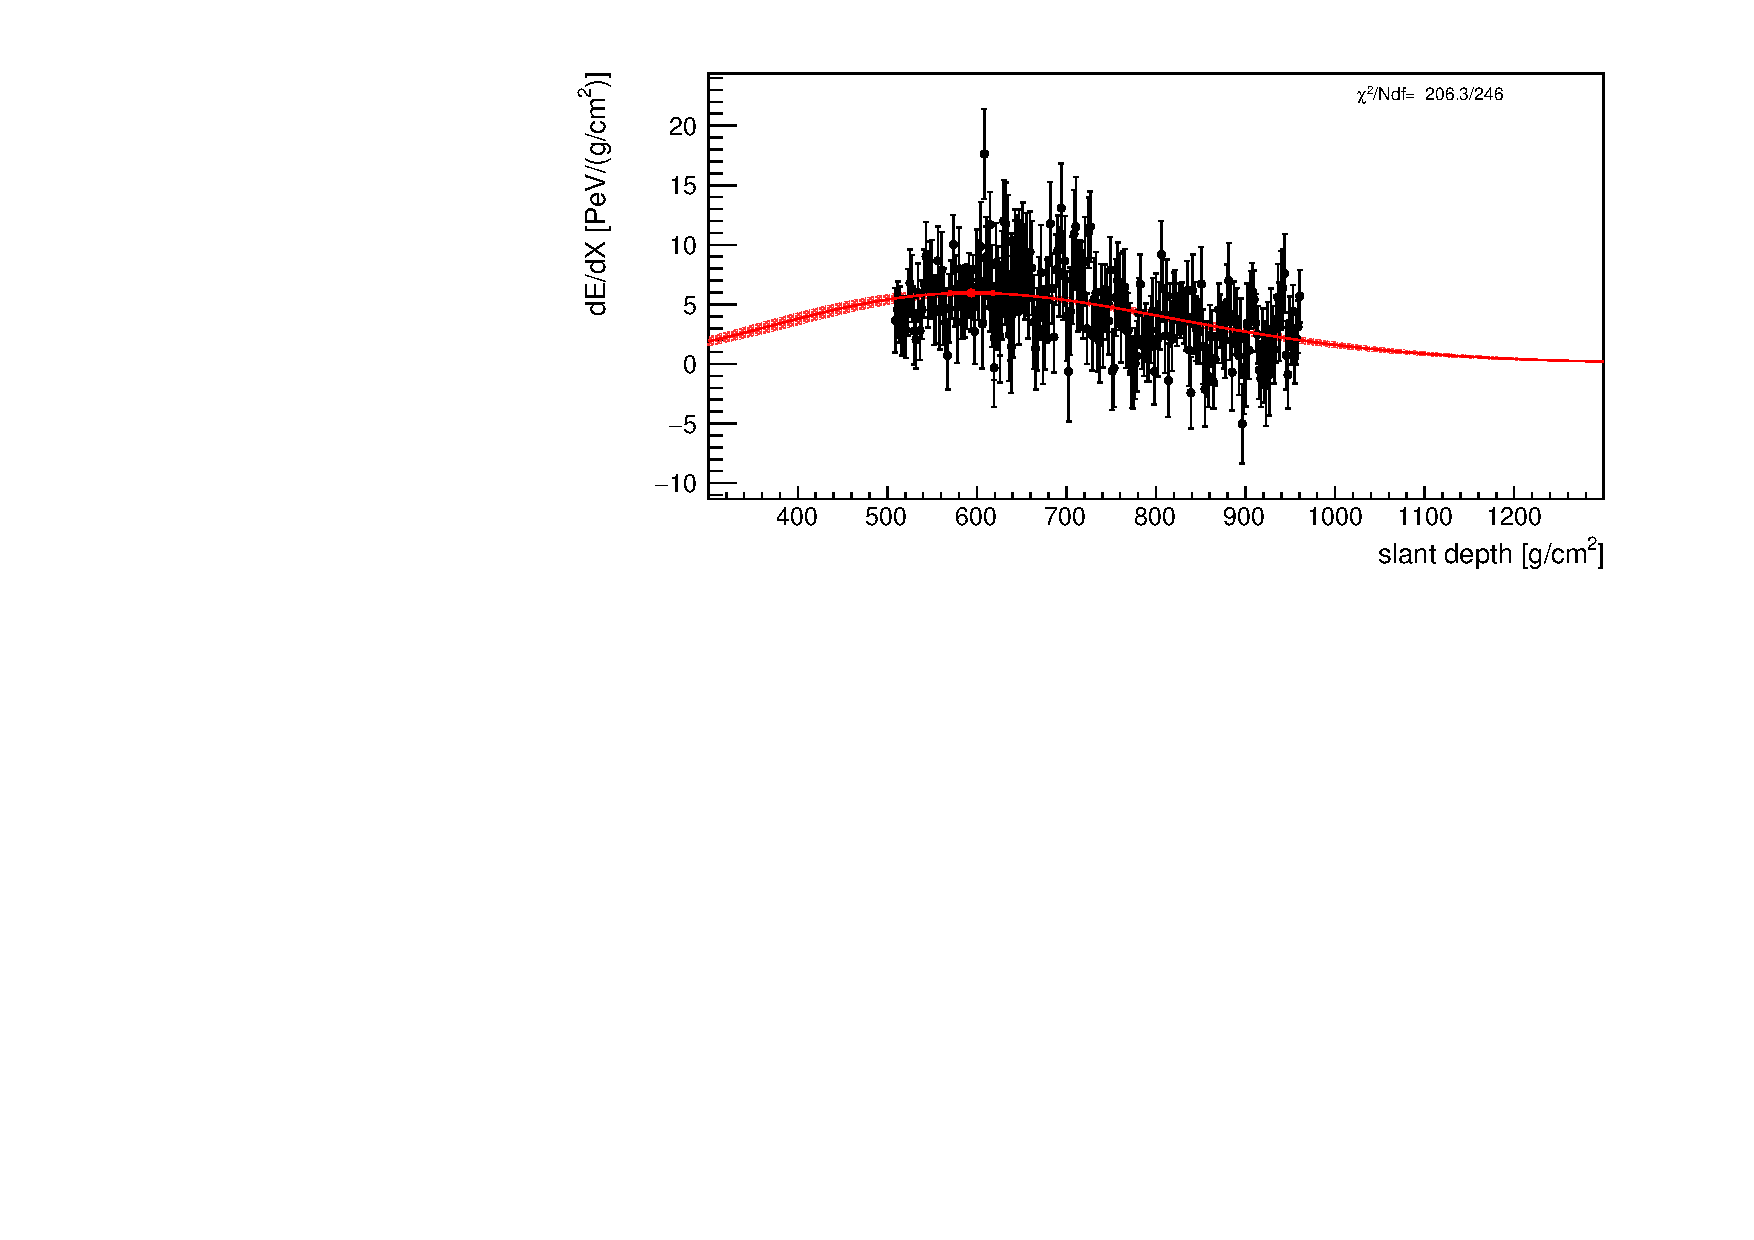
\includegraphics[width=\textwidth]{/home/tsudholz/PhD/Thesis/chapters/graphs/CloudFlags/CloudCut_Events_Failed/Auger_70735278500_SlantDepth.pdf}
  \caption{FD profile of the energy deposited as a function of atmospheric depth.}
  \end{subfigure}
 \vspace{0.5cm}
  \begin{subfigure}[b]{0.45\textwidth}
  	\centering
  	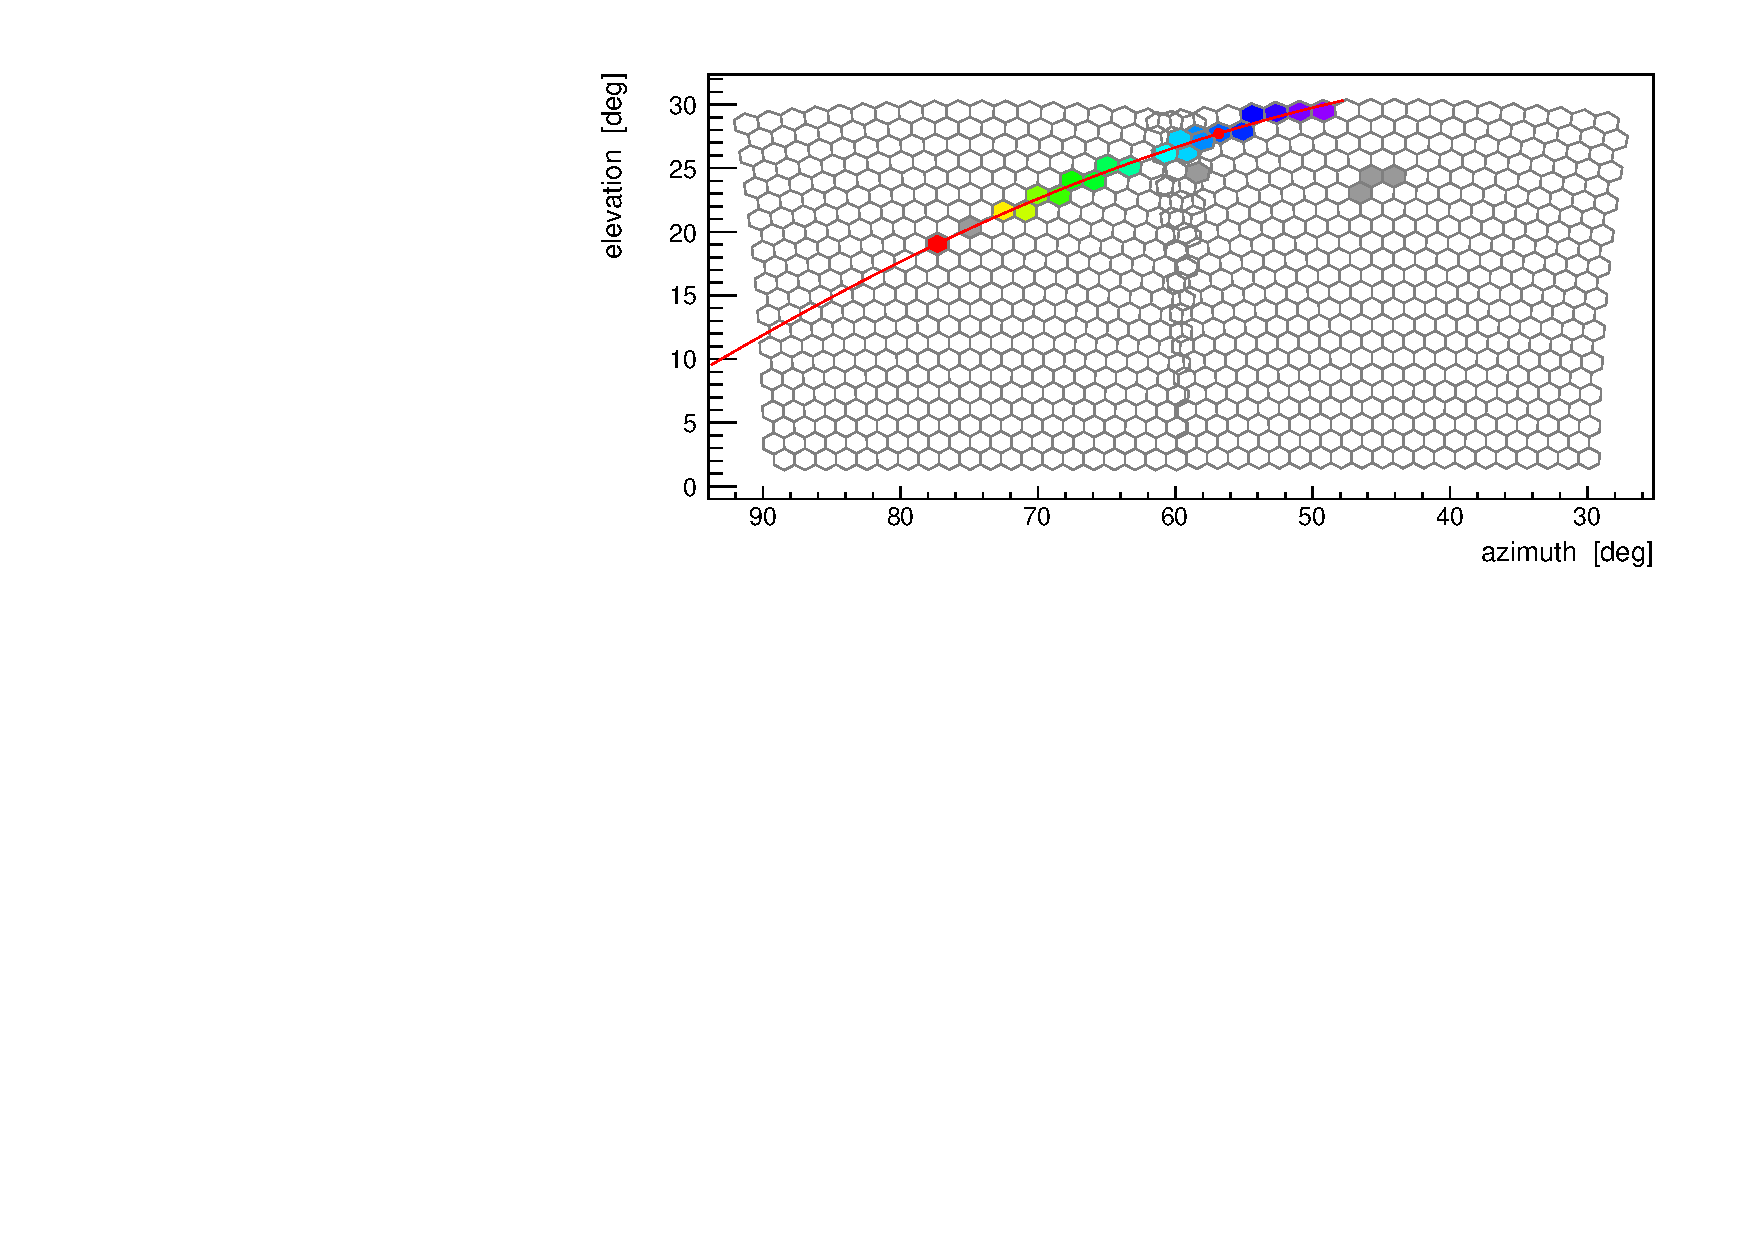
\includegraphics[width=\textwidth , height=\tempheight]{/home/tsudholz/PhD/Thesis/chapters/graphs/CloudFlags/CloudCut_Events_Failed/Auger_70735278500_FdProfile.pdf}
  	\caption{FD light profile}
  \end{subfigure}
  \begin{subfigure}[b]{0.45\textwidth}
  	\centering
  	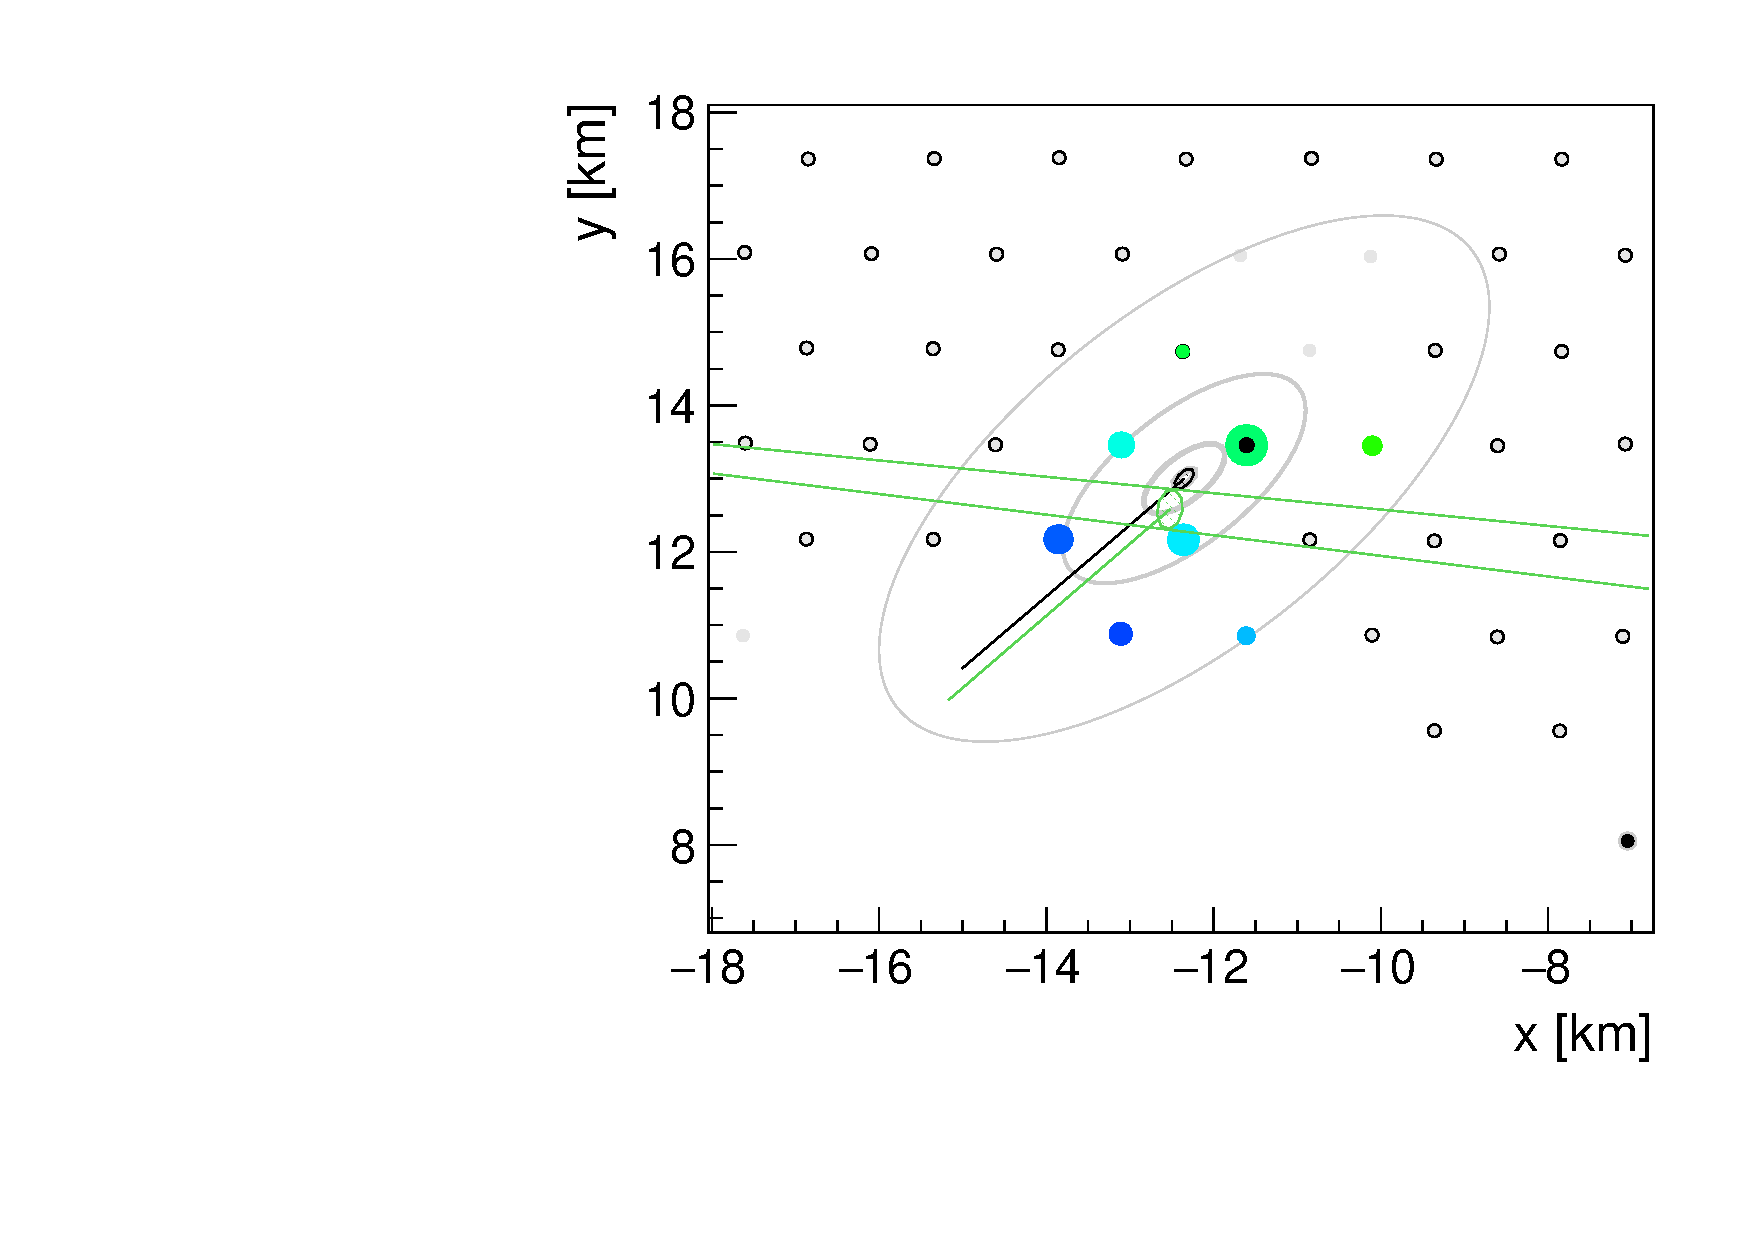
\includegraphics[width=0.8\textwidth , height=\tempheight]{/home/tsudholz/PhD/Thesis/chapters/graphs/CloudFlags/CloudCut_Events_Failed/Auger_70735278500_SdProfile.pdf}
  	\caption{SD tank triggered profile}
  \end{subfigure}

  \begin{subfigure}[b]{0.45\textwidth}
  	\centering
	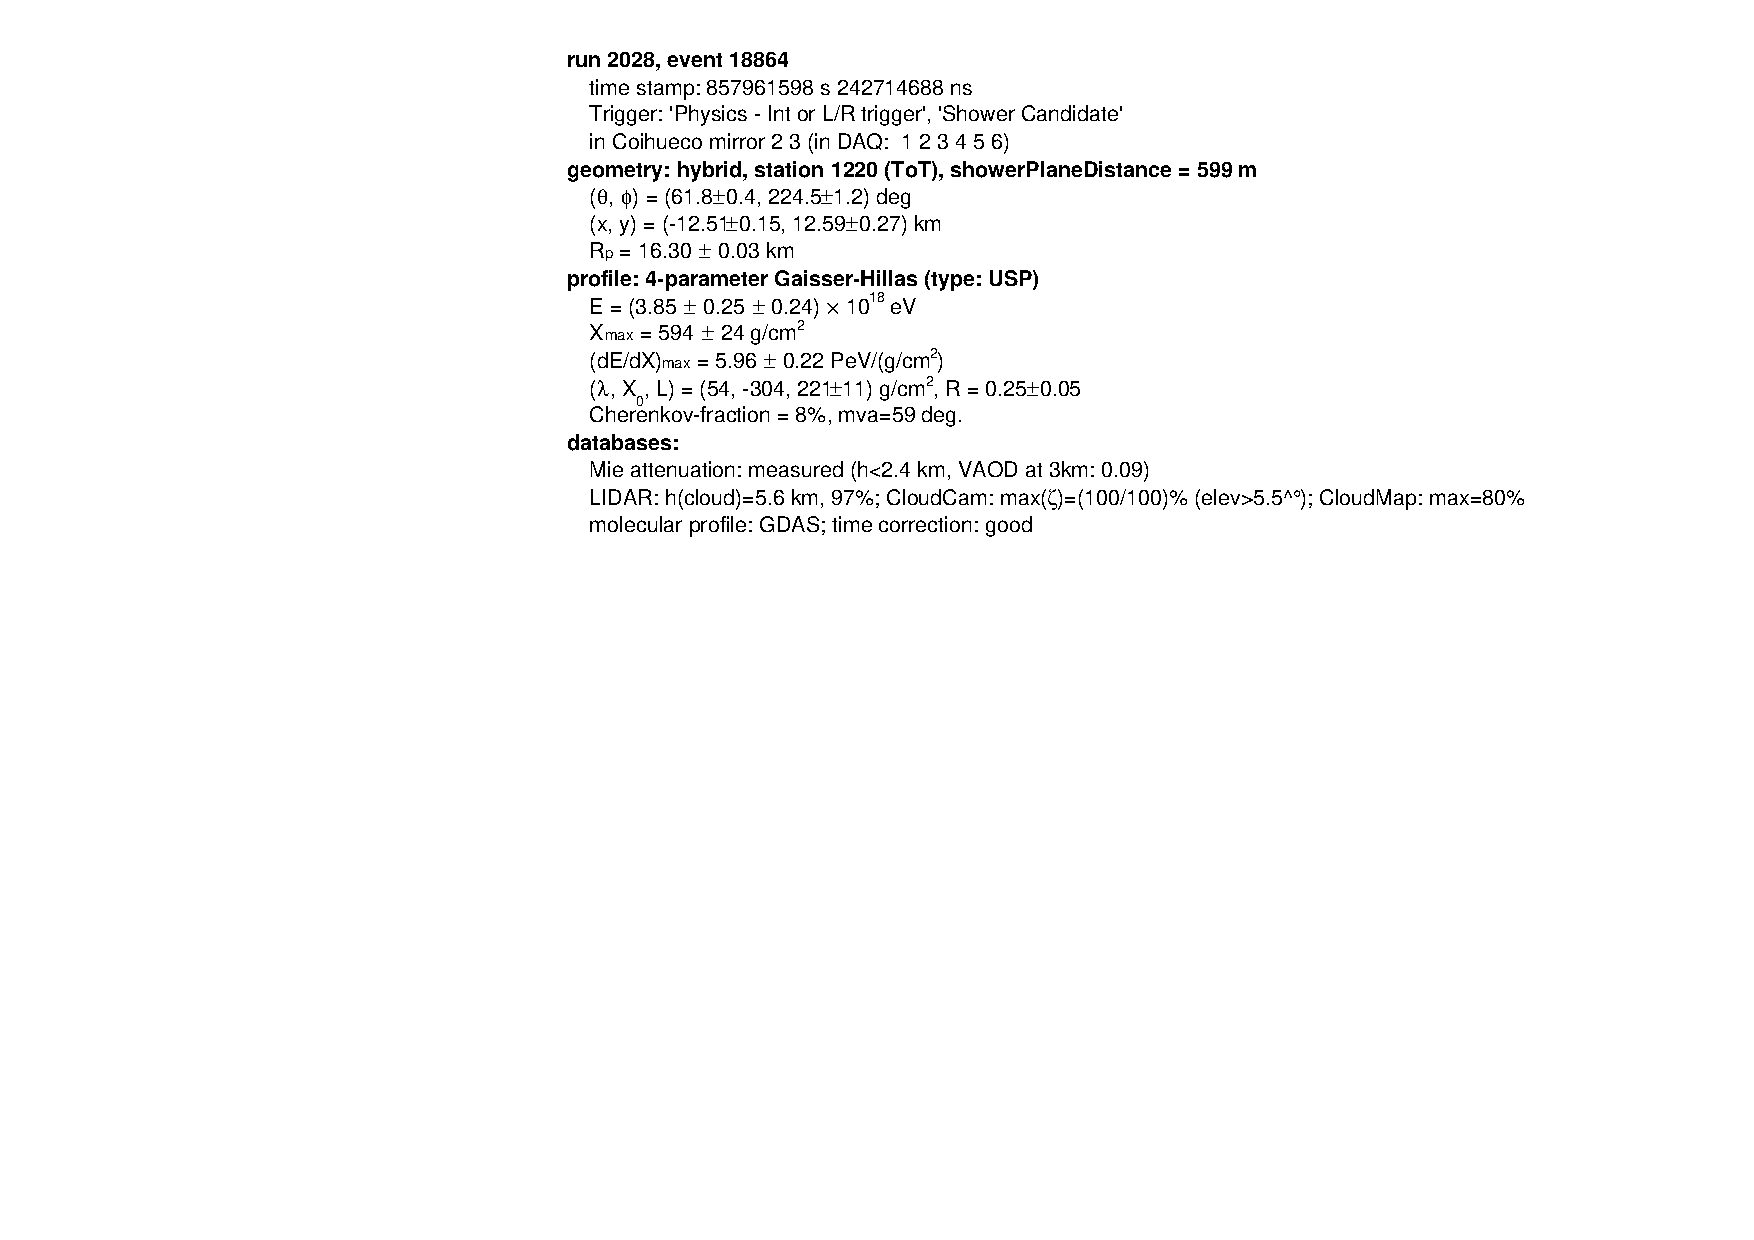
\includegraphics[height=\tempheight , trim = 0 0 5.5cm 0]{/home/tsudholz/PhD/Thesis/chapters/graphs/CloudFlags/CloudCut_Events_Failed/Auger_70735278500_FdEventInfo.pdf}
  	\caption{FD light profile}
  \end{subfigure}
  \begin{subfigure}[b]{0.45\textwidth}
  	\centering
	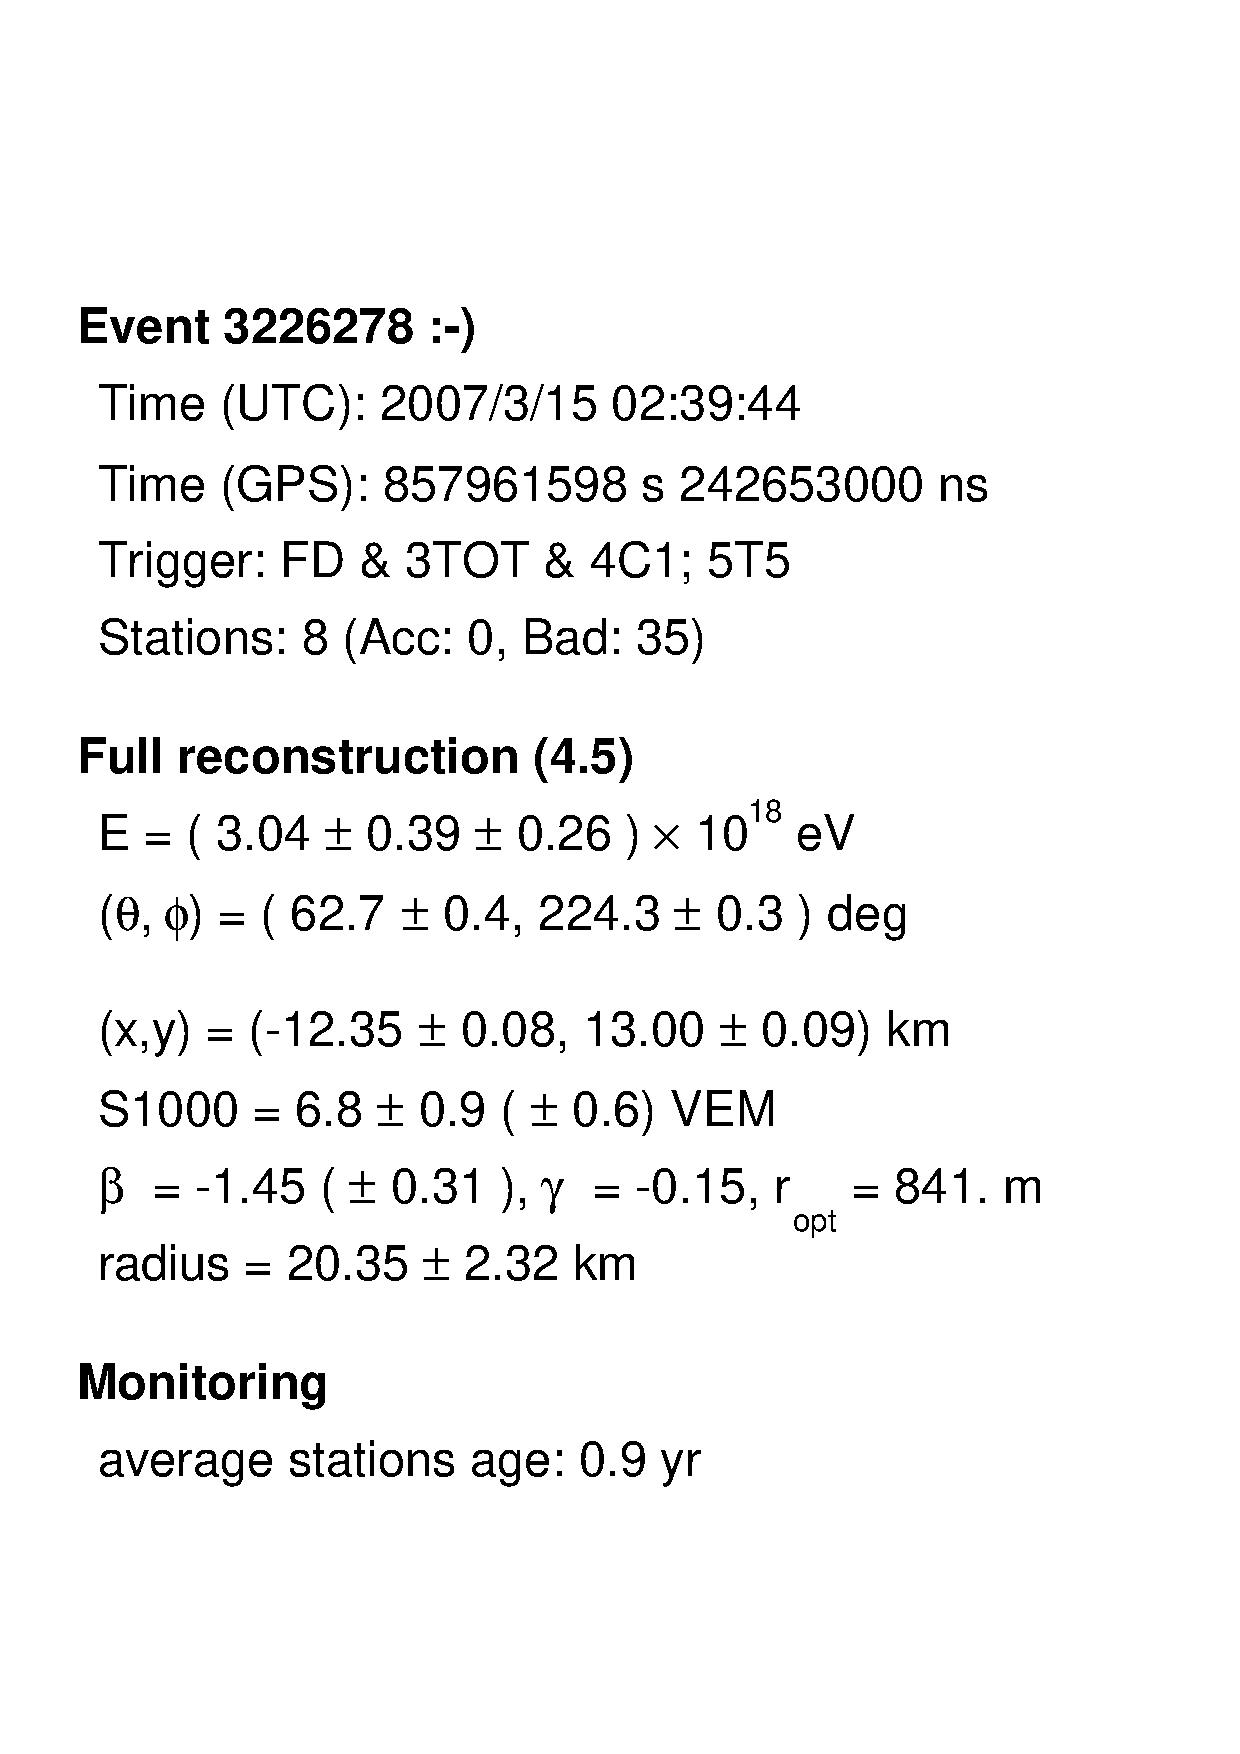
\includegraphics[height=\tempheight]{/home/tsudholz/PhD/Thesis/chapters/graphs/CloudFlags/CloudCut_Events_Failed/Auger_70735278500_SdEventInfo.pdf}
  	\caption{SD tank triggered profile}
  \end{subfigure}
  \caption{Example of an Auger event that would fail the cloud selection cut from EventBrowser}
\end{figure}

\begin{figure}[!p]
\centering
  \settoheight{\tempheight}{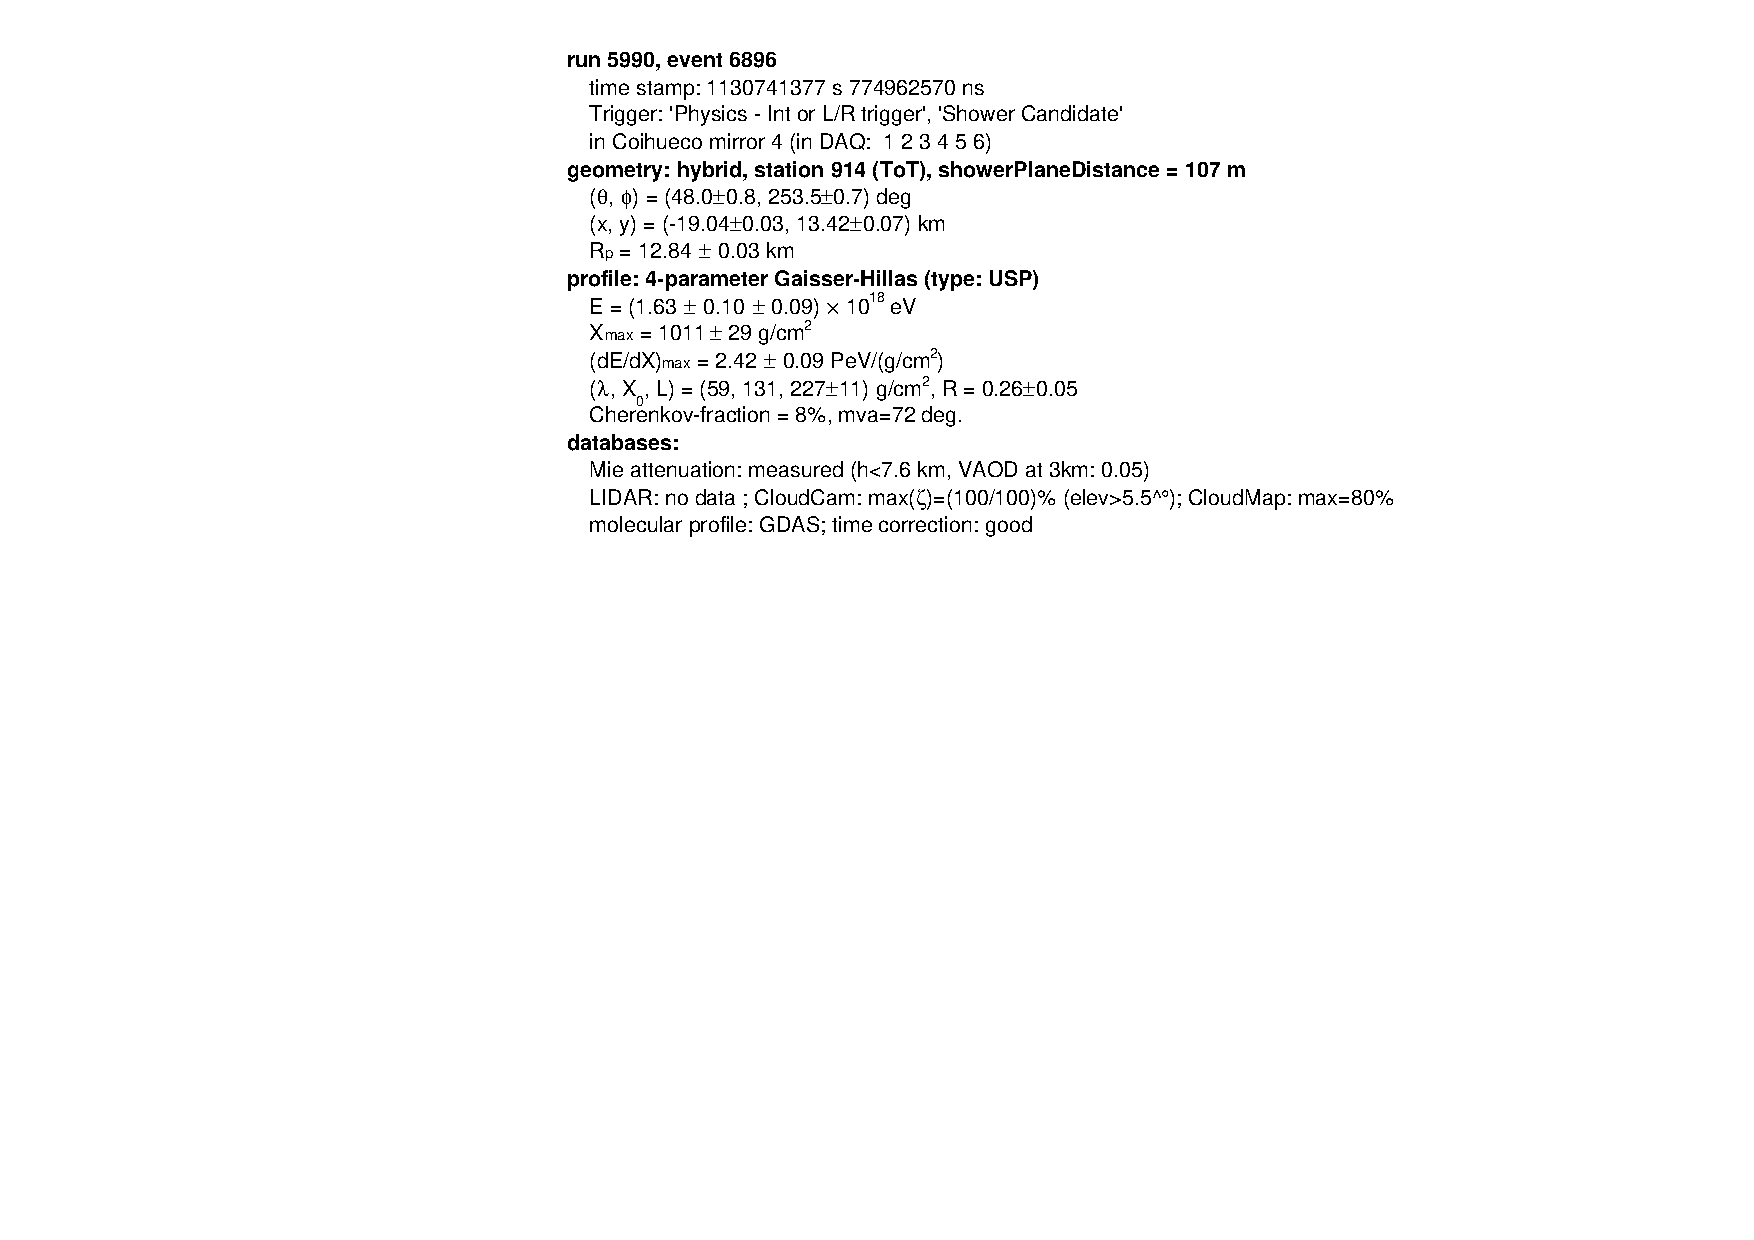
\includegraphics[width=0.45\textwidth , trim = 0 0 5.5cm 0]{/home/tsudholz/PhD/Thesis/chapters/graphs/CloudFlags/CloudCut_Events_Failed/Auger_153086776200_FdEventInfo.pdf}}
 \vspace{2cm}
  \begin{subfigure}[b]{\textwidth}
  \centering
  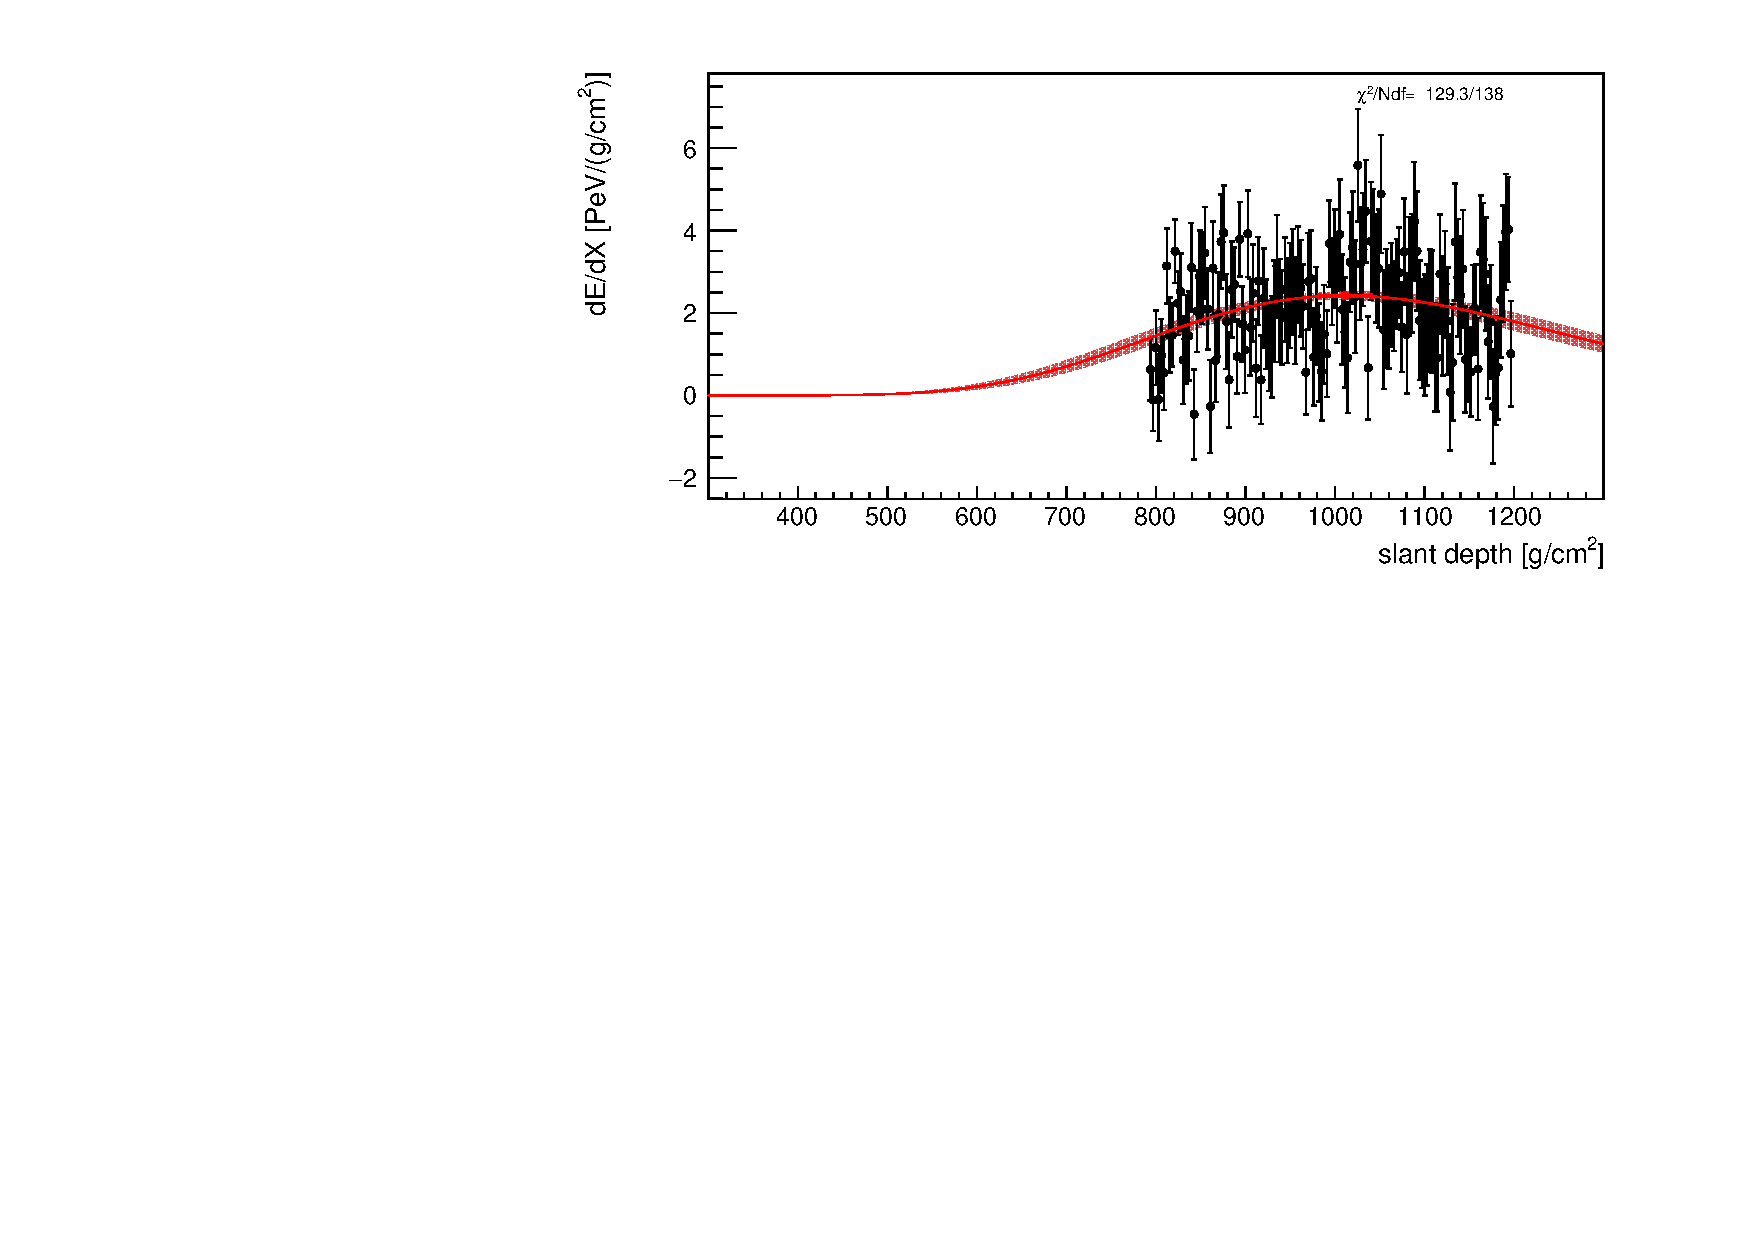
\includegraphics[width=\textwidth]{/home/tsudholz/PhD/Thesis/chapters/graphs/CloudFlags/CloudCut_Events_Failed/Auger_153086776200_SlantDepth.pdf}
  \caption{FD profile of the energy deposited as a function of atmospheric depth.}
  \end{subfigure}
 \vspace{0.5cm}
  \begin{subfigure}[b]{0.45\textwidth}
  	\centering
  	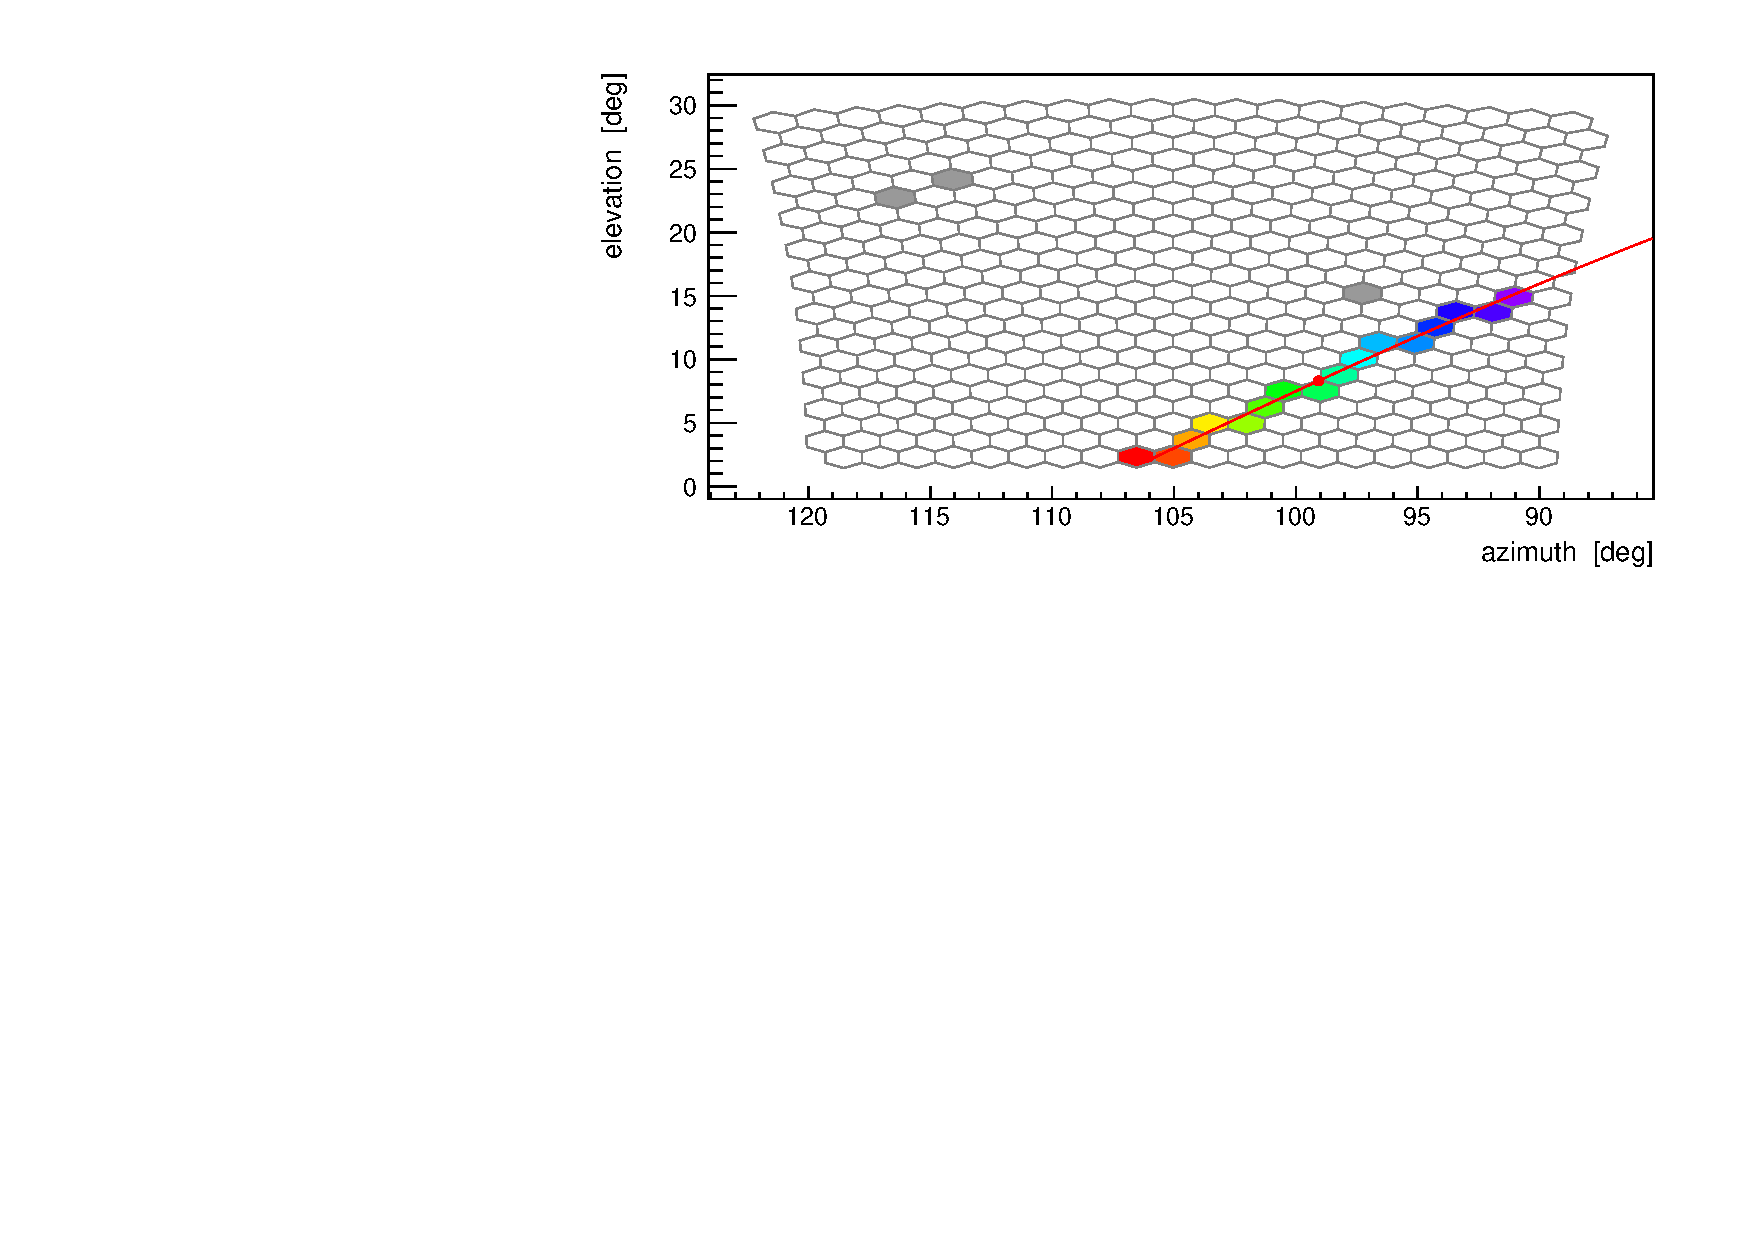
\includegraphics[width=\textwidth , height=\tempheight]{/home/tsudholz/PhD/Thesis/chapters/graphs/CloudFlags/CloudCut_Events_Failed/Auger_153086776200_FdProfile.pdf}
  	\caption{FD light profile}
  \end{subfigure}
  \begin{subfigure}[b]{0.45\textwidth}
  	\centering
  	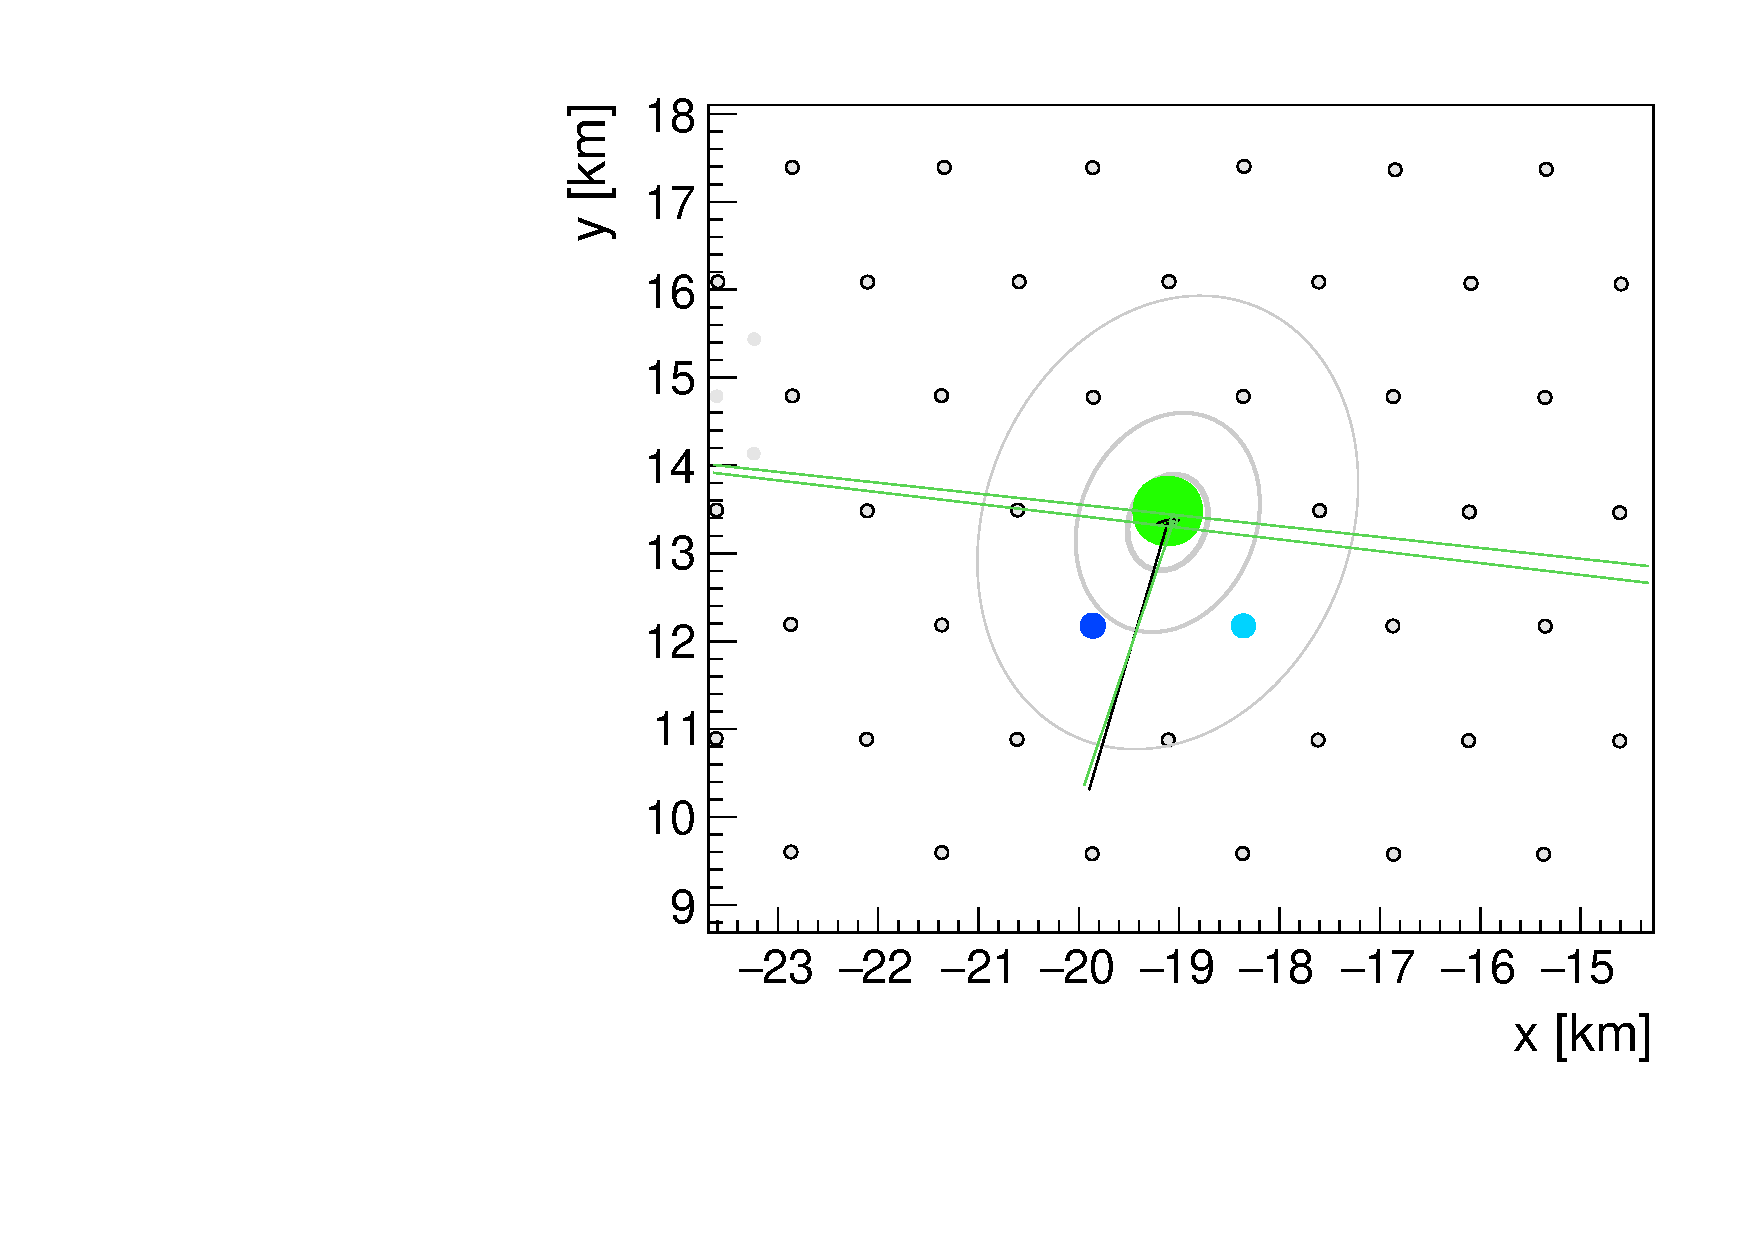
\includegraphics[width=0.8\textwidth , height=\tempheight]{/home/tsudholz/PhD/Thesis/chapters/graphs/CloudFlags/CloudCut_Events_Failed/Auger_153086776200_SdProfile.pdf}
  	\caption{SD tank triggered profile}
  \end{subfigure}

  \begin{subfigure}[b]{0.45\textwidth}
  	\centering
	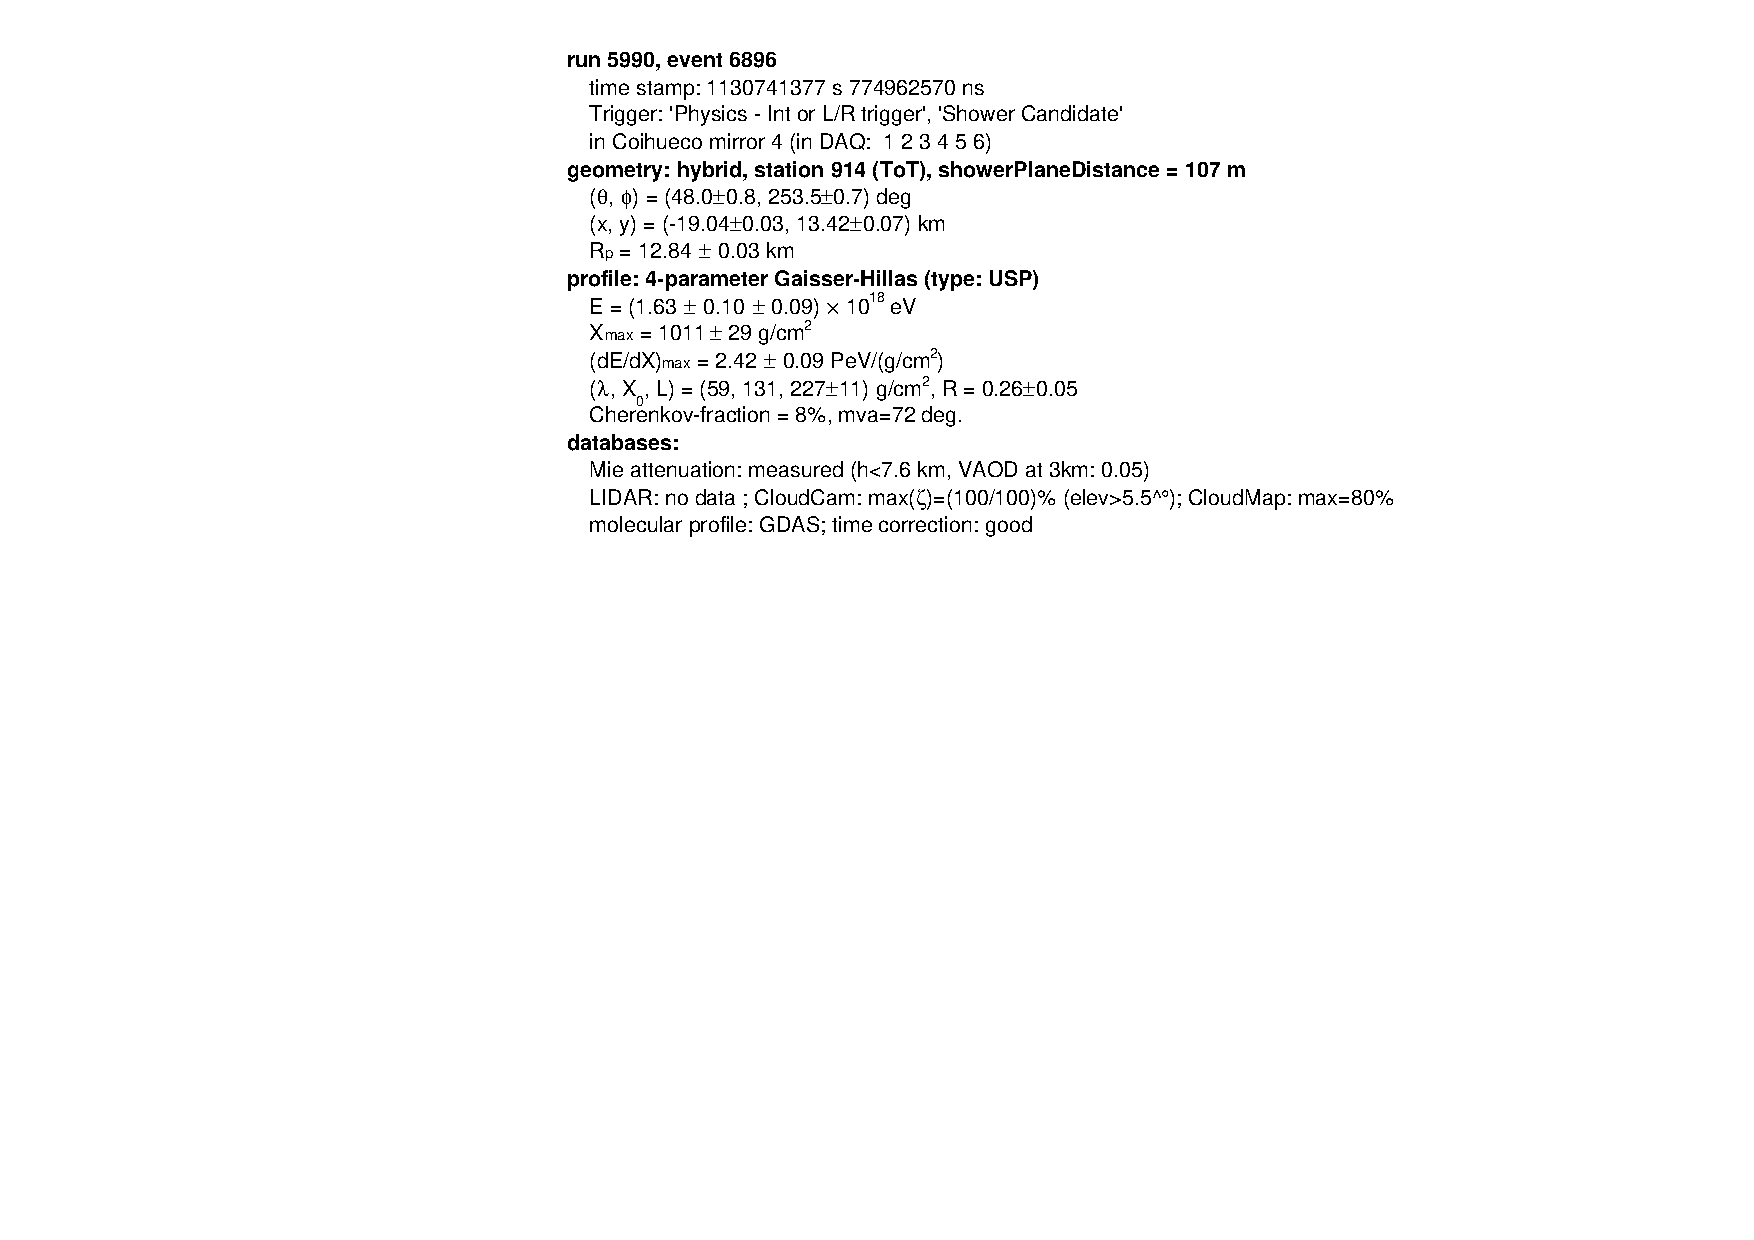
\includegraphics[height=\tempheight , trim = 0 0 5.5cm 0]{/home/tsudholz/PhD/Thesis/chapters/graphs/CloudFlags/CloudCut_Events_Failed/Auger_153086776200_FdEventInfo.pdf}
  	\caption{FD light profile}
  \end{subfigure}
  \begin{subfigure}[b]{0.45\textwidth}
  	\centering
	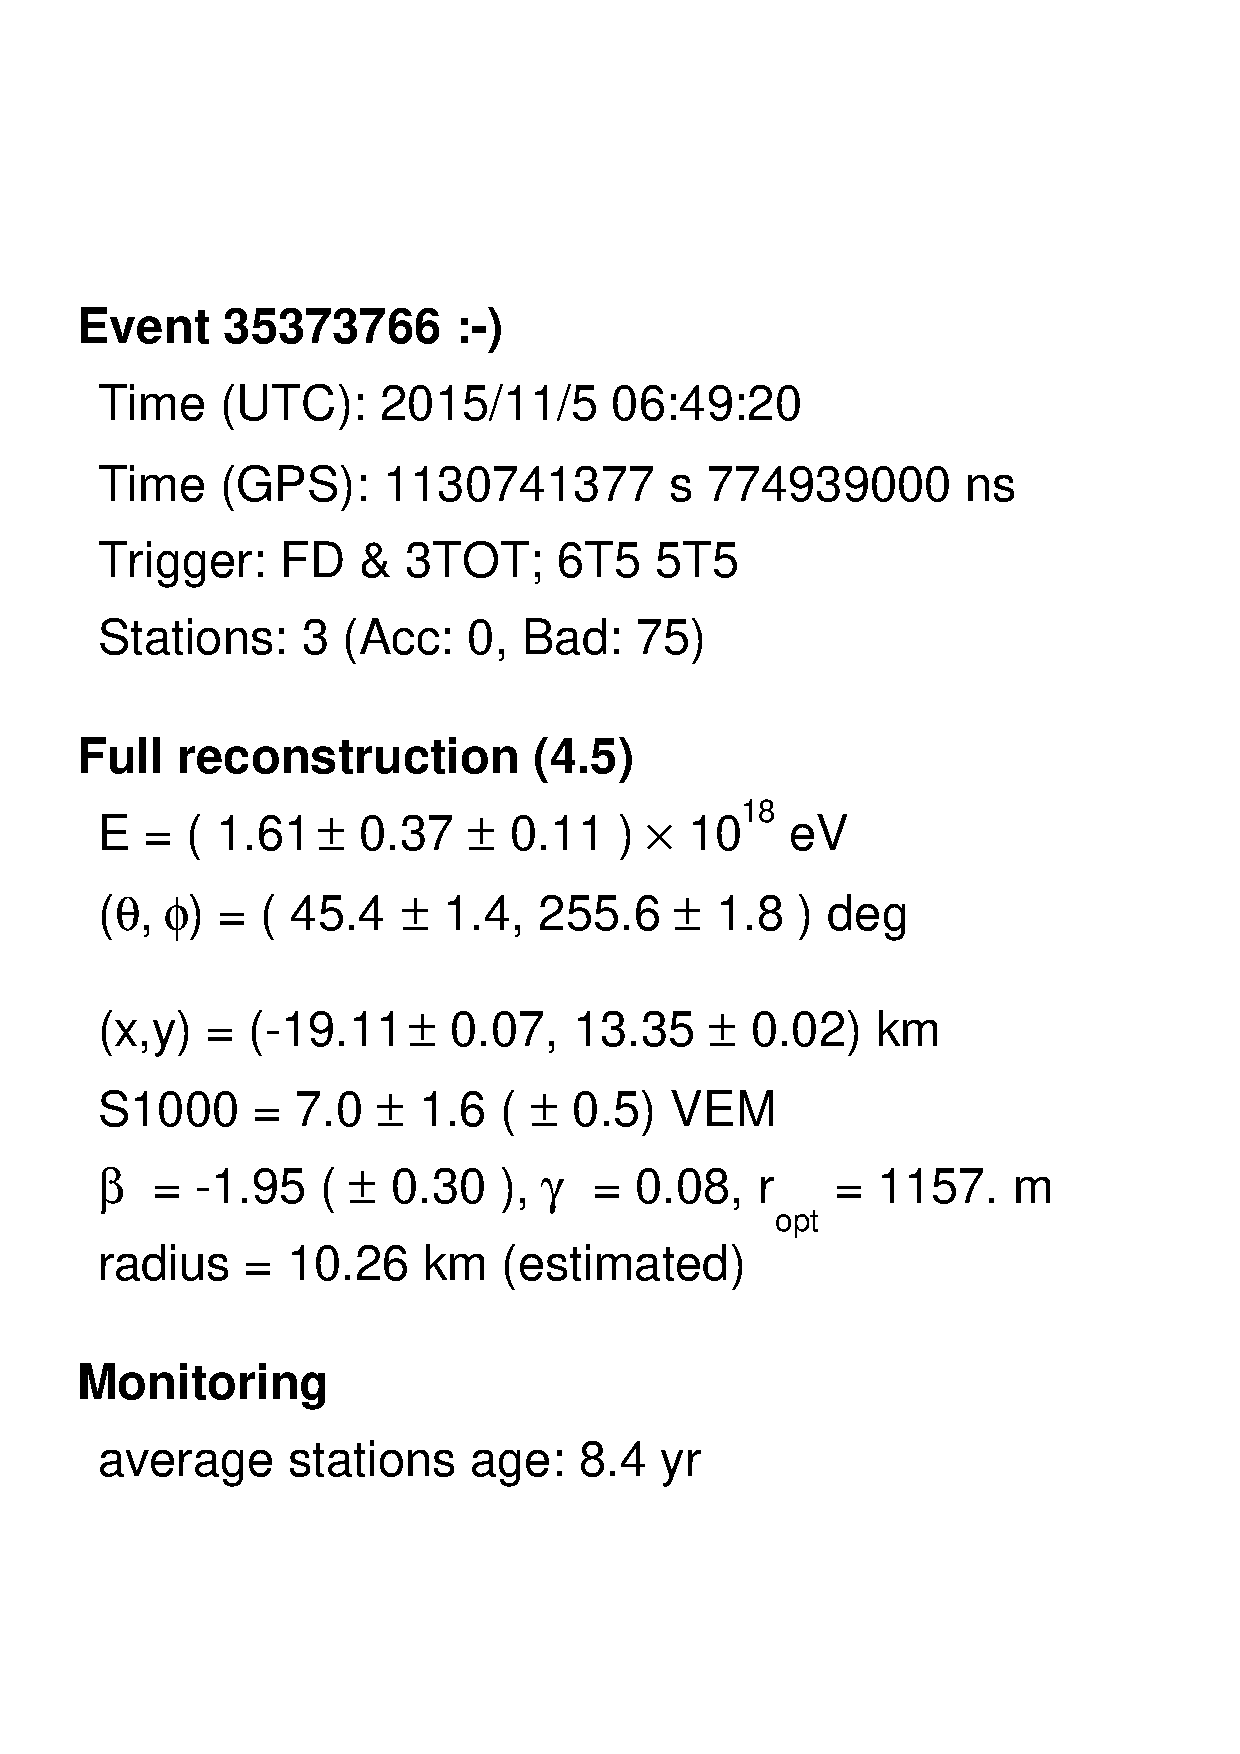
\includegraphics[height=\tempheight]{/home/tsudholz/PhD/Thesis/chapters/graphs/CloudFlags/CloudCut_Events_Failed/Auger_153086776200_SdEventInfo.pdf}
  	\caption{SD tank triggered profile}
  \end{subfigure}
  \caption{Example of an Auger event that would fail the cloud selection cut from EventBrowser}
\end{figure}


% Events that would all quality cuts including the cloud cut

\begin{figure}[h]
\centering
  \settoheight{\tempheight}{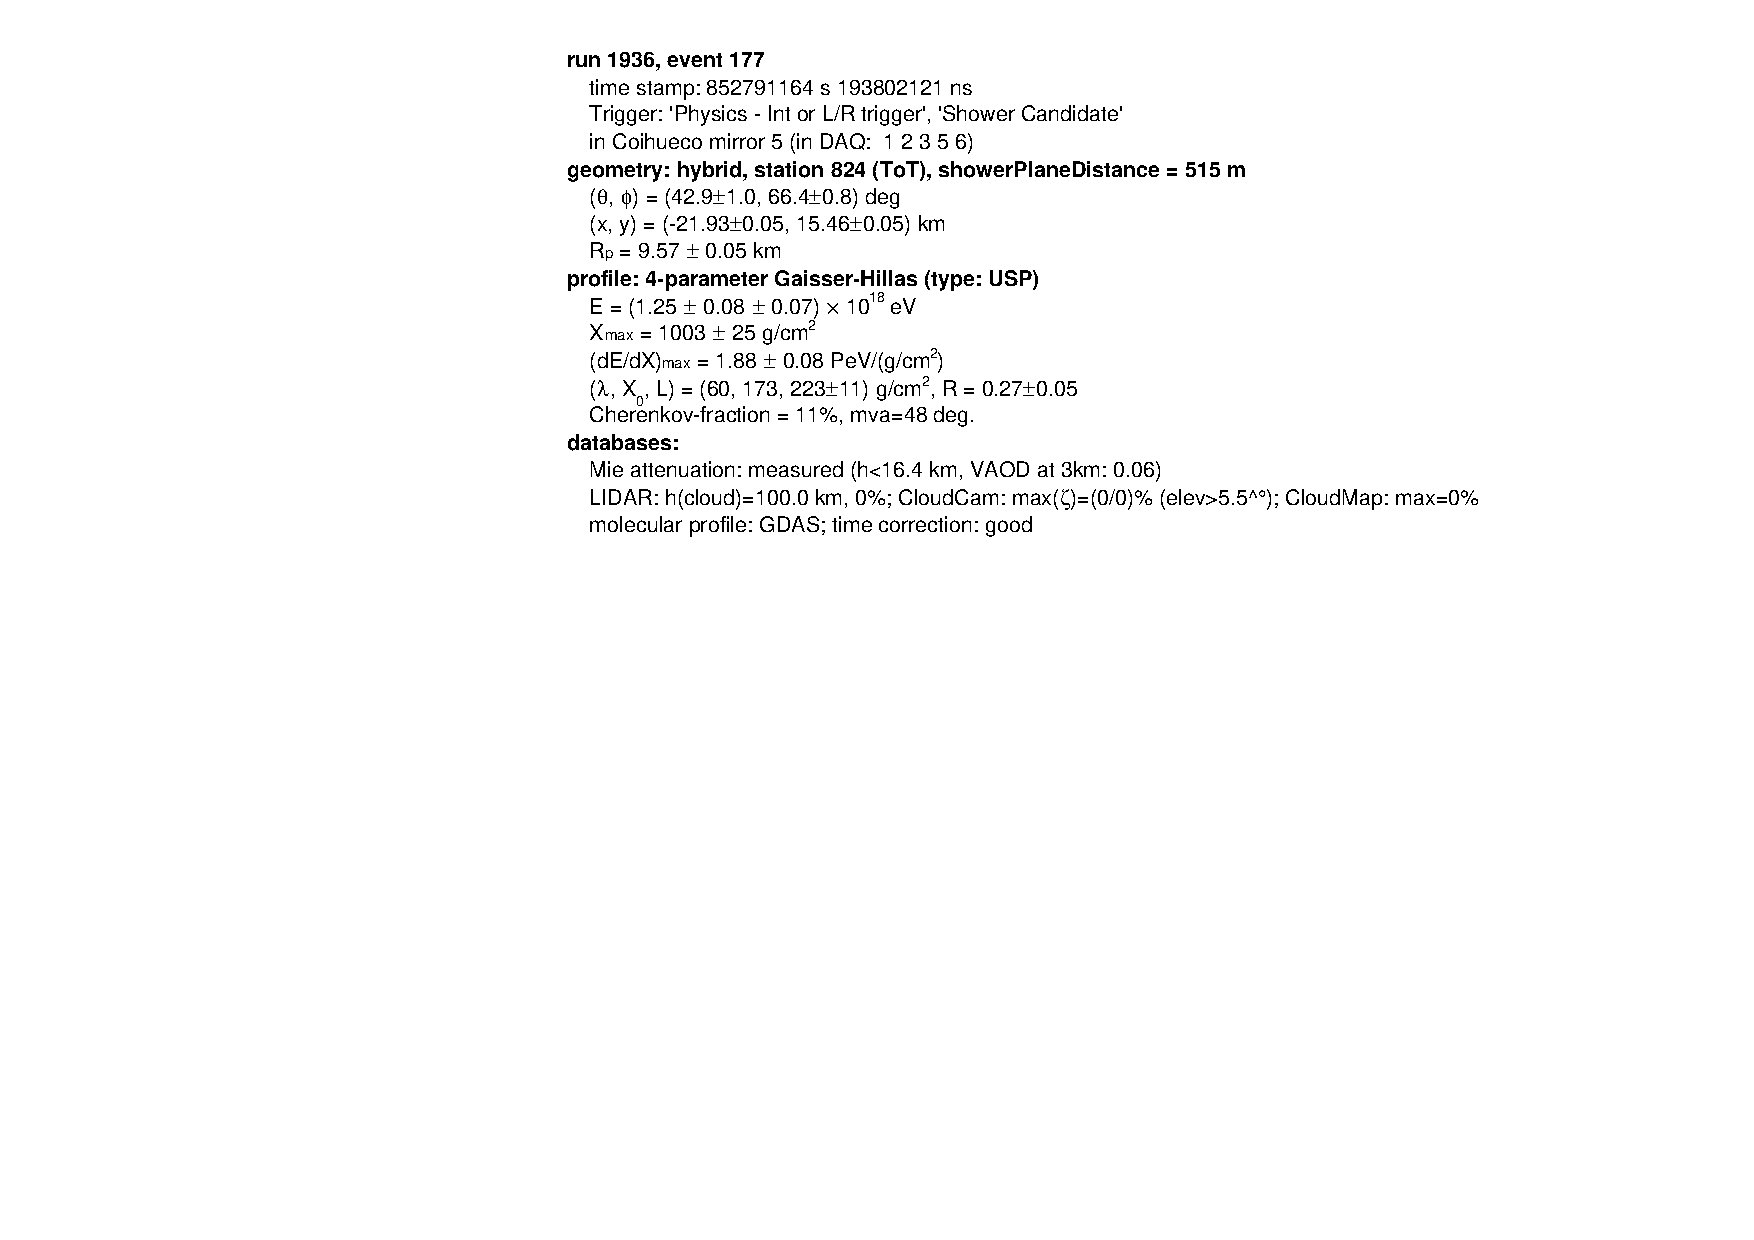
\includegraphics[width=0.45\textwidth , trim = 0 0 5.5cm 0]{/home/tsudholz/PhD/Thesis/chapters/graphs/CloudFlags/CloudCut_Events/Auger_70136635100_FdEventInfo.pdf}}
 \vspace{2cm}
  \begin{subfigure}[b]{\textwidth}
  \centering
  \includegraphics[width=\textwidth]{/home/tsudholz/PhD/Thesis/chapters/graphs/CloudFlags/CloudCut_Events/Auger_70136635100_SlantDepth.pdf}
  \caption{FD profile of the energy deposited as a function of atmospheric depth.}
  \end{subfigure}
 \vspace{0.5cm}
  \begin{subfigure}[b]{0.45\textwidth}
  	\centering
  	\includegraphics[width=\textwidth , height=\tempheight]{/home/tsudholz/PhD/Thesis/chapters/graphs/CloudFlags/CloudCut_Events/Auger_70136635100_FdProfile.pdf}
  	\caption{FD light profile}
  \end{subfigure}
  \begin{subfigure}[b]{0.45\textwidth}
  	\centering
  	\includegraphics[width=0.8\textwidth , height=\tempheight]{/home/tsudholz/PhD/Thesis/chapters/graphs/CloudFlags/CloudCut_Events/Auger_70136635100_SdProfile.pdf}
  	\caption{SD tank triggered profile}
  \end{subfigure}

  \begin{subfigure}[b]{0.45\textwidth}
  	\centering
	\includegraphics[height=\tempheight , trim = 0 0 5.5cm 0]{/home/tsudholz/PhD/Thesis/chapters/graphs/CloudFlags/CloudCut_Events/Auger_70136635100_FdEventInfo.pdf}
  	\caption{FD light profile}
  \end{subfigure}
  \begin{subfigure}[b]{0.45\textwidth}
  	\centering
	\includegraphics[height=\tempheight]{/home/tsudholz/PhD/Thesis/chapters/graphs/CloudFlags/CloudCut_Events/Auger_70136635100_SdEventInfo.pdf}
  	\caption{SD tank triggered profile}
  \end{subfigure}
  \caption{Example of an Auger event that would pass the cloud selection cut from EventBrowser}
\end{figure}

\begin{figure}[h]
\centering
  \settoheight{\tempheight}{\includegraphics[width=0.45\textwidth , trim = 0 0 5.5cm 0]{/home/tsudholz/PhD/Thesis/chapters/graphs/CloudFlags/CloudCut_Events/Auger_101576030600_FdEventInfo.pdf}}
 \vspace{2cm}
  \begin{subfigure}[b]{\textwidth}
  \centering
  \includegraphics[width=\textwidth]{/home/tsudholz/PhD/Thesis/chapters/graphs/CloudFlags/CloudCut_Events/Auger_101576030600_SlantDepth.pdf}
  \caption{FD profile of the energy deposited as a function of atmospheric depth.}
  \end{subfigure}
 \vspace{0.5cm}
  \begin{subfigure}[b]{0.45\textwidth}
  	\centering
  	\includegraphics[width=\textwidth , height=\tempheight]{/home/tsudholz/PhD/Thesis/chapters/graphs/CloudFlags/CloudCut_Events/Auger_101576030600_FdProfile.pdf}
  	\caption{FD light profile}
  \end{subfigure}
  \begin{subfigure}[b]{0.45\textwidth}
  	\centering
  	\includegraphics[width=0.8\textwidth , height=\tempheight]{/home/tsudholz/PhD/Thesis/chapters/graphs/CloudFlags/CloudCut_Events/Auger_101576030600_SdProfile.pdf}
  	\caption{SD tank triggered profile}
  \end{subfigure}

  \begin{subfigure}[b]{0.45\textwidth}
  	\centering
	\includegraphics[height=\tempheight , trim = 0 0 5.5cm 0]{/home/tsudholz/PhD/Thesis/chapters/graphs/CloudFlags/CloudCut_Events/Auger_101576030600_FdEventInfo.pdf}
  	\caption{FD light profile}
  \end{subfigure}
  \begin{subfigure}[b]{0.45\textwidth}
  	\centering
	\includegraphics[height=\tempheight]{/home/tsudholz/PhD/Thesis/chapters/graphs/CloudFlags/CloudCut_Events/Auger_101576030600_SdEventInfo.pdf}
  	\caption{SD tank triggered profile}
  \end{subfigure}
  \caption{Example of an Auger event that would pass the cloud selection cut from EventBrowser}
\end{figure}

\begin{figure}[h]
\centering
  \settoheight{\tempheight}{\includegraphics[width=0.45\textwidth , trim = 0 0 5.5cm 0]{/home/tsudholz/PhD/Thesis/chapters/graphs/CloudFlags/CloudCut_Events/Auger_92285877600_FdEventInfo.pdf}}
 \vspace{2cm}
  \begin{subfigure}[b]{\textwidth}
  \centering
  \includegraphics[width=\textwidth]{/home/tsudholz/PhD/Thesis/chapters/graphs/CloudFlags/CloudCut_Events/Auger_92285877600_SlantDepth.pdf}
  \caption{FD profile of the energy deposited as a function of atmospheric depth.}
  \end{subfigure}
 \vspace{0.5cm}
  \begin{subfigure}[b]{0.45\textwidth}
  	\centering
  	\includegraphics[width=\textwidth , height=\tempheight]{/home/tsudholz/PhD/Thesis/chapters/graphs/CloudFlags/CloudCut_Events/Auger_92285877600_FdProfile.pdf}
  	\caption{FD light profile}
  \end{subfigure}
  \begin{subfigure}[b]{0.45\textwidth}
  	\centering
  	\includegraphics[width=0.8\textwidth , height=\tempheight]{/home/tsudholz/PhD/Thesis/chapters/graphs/CloudFlags/CloudCut_Events/Auger_92285877600_SdProfile.pdf}
  	\caption{SD tank triggered profile}
  \end{subfigure}

  \begin{subfigure}[b]{0.45\textwidth}
  	\centering
	\includegraphics[height=\tempheight , trim = 0 0 5.5cm 0]{/home/tsudholz/PhD/Thesis/chapters/graphs/CloudFlags/CloudCut_Events/Auger_92285877600_FdEventInfo.pdf}
  	\caption{FD light profile}
  \end{subfigure}
  \begin{subfigure}[b]{0.45\textwidth}
  	\centering
	\includegraphics[height=\tempheight]{/home/tsudholz/PhD/Thesis/chapters/graphs/CloudFlags/CloudCut_Events/Auger_92285877600_SdEventInfo.pdf}
  	\caption{SD tank triggered profile}
  \end{subfigure}
  \caption{Example of an Auger event that would pass the cloud selection cut from EventBrowser}
\end{figure}

% Explanation of graphs.

Example set of events that would either pass or fail the cloud flags. The events are here to show graphically the events that are observed and the reconstructed information. I focused on events in the tails of the Xmax distributions to show here. I restricted my search to events with Xmax either greater than 1000 g/cm$^{2}$ or less than 600 g/cm$^{2}$. In the tails, there was a lot of visual overlap with the events with reconstructed Xmax greater than 1000 g/cm$^{2}$ if they would or would not pass the cloud flag cut. While events with reconstructed Xmax less than 600 g/cm$^{2}$ and would pass the cloud cut seemed to a different distribution to ones that would fail the cloud flag cut.

Shown here are two examples of events with reconstructed Xmax less than 600 g/cm$^{2}$ and one event with a Xmax greater than 1000 g/cm$^{2}$ that would fail the cloud flag cut. I have also shown two events of interest with Xmax less than 600 g/cm$^{2}$ and one event with Xmax greater than 1000 g/cm$^{2}$ that would pass the cloud flag cut.

\section{Discussion}

%Gaining 30\% more events cut is removed

%Have to be careful of outliers

%Mean Xmax and spread in Xmax does not change significantly

%With cloud cut confident that events that could be cloud effected are removed. Without the cloud cut no significant impact is seem expect for the increase of statistics by 30\%.
%
%May need more investigation for any analysis dealing with mass composition but may be ok for other analyses where an increase in statistics are useful and not as concerned over the tails of the distribution. 
%
%Major of accepted events are accepted from data collected by the IR cloud cameras. Interestingly only a small fraction of events are unclassified due to a lack of cloud monitoring data from any source.
%
%The normalised Xmax distribution 

It was interesting to see that the majority of events are accepted by passing cloud cuts from data provided by the infra-red cloud cameras. There was only a small fraction of events that do not have any cloud camera data associated with it where the event would still pass all of the other quality cuts. 

Across all of the energy bins shown in the results there would be an increase in event of 30\% if the cloud cut was removed. This would be of great benefit to the highest energy bin (E $>$ 10$^{19.5}$ eV) where the statistics are low. From the graphs shown in the results, the means and standard deviations are not significantly different from the distributions when the cloud cuts are applied.

From the results, it can be seen that this cut could be removed for studies that would benefit from the increased statistics. A study where more care would need to be investigated would be studies into mass compositions. Mass composition is sensitive to changes in the standard deviation so outliers in the distribution are of concern. I looked at events with Xmax greater than 1000 g/cm$^2$ and less than 600 g/cm$^2$ to compare the tails of distributions. It was observed that there was overlapping events in the events with Xmax greater than 1000 g/cm$^2$


\section{Conclusion}
